In this chapter we illustrate how we tested each of our modules and their integration. We also show the results of our experiments and follow them with a discussion. This chapter deals with the main three modules presented previously throughout the thesis: autonomous functionalities, communication and collaboration techniques. 

In testing autonomous functionalities and system integration on ROS,
we verified that the sub-modules are working properly by comparing the expected outcomes from every module discussed in the methodology, to the results generated from actual testing on the simulation environments: Gazebo and RViz. For every module, we designed scenarios and test cases that verifies a list of checks and discussed them briefly. Then we analyze whether the results are consistent with the expected outcomes or not. If they are consistent, then the module is verified and is discussed whether it needs some modification to improve the results. If they were not consistent, the reasons were explained.

In testing our RL models, we quantify their effect on the system's main metric: EV travel time, in the SUMO simulation environment.


\label{SecProjTest}

%-----------------------------------------------------%
%-----------------------------------------------------%
%-----------------------------------------------------%

\section{Autonomous Functionalities}
\label{sec:test_aut_func}

\subsection{Mapping and Localization}
\label{test_loc_map}
\begin{enumerate}
\item \textbf{Mapping} 
\\
As mentioned in section \ref{method_loc_map}, we used GIMP \cite{gimp} to refine the generated map. Below are the results for the map before and after refining it.\\
\begin{figure}[h]
    \begin{subfigure}{1\textwidth}
    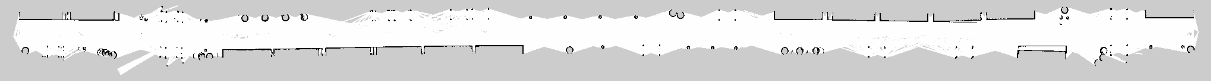
\includegraphics[width=1\linewidth]{images/finalMap.png}
    \caption{Resulted map before editing with GIMP.}
    \label{fig:map_before_gimp}
    \end{subfigure}

    \begin{subfigure}{1\textwidth}
    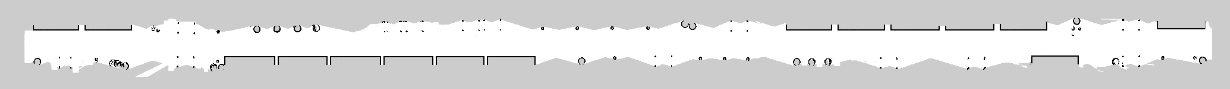
\includegraphics[width=1\linewidth]{images/finalMap_gimp.png}
    \caption{Resulted map after editing with GIMP.}
    \label{fig:map_after_gimp}
    \end{subfigure}

    \caption{Resulted map generated from Gmapping.}
    \label{fig:resulted_map}
    \end{figure}
    \leavevmode
\item\textbf{Localization}
\\
As for testing the vehicle's localization discussed in \ref{method_loc_map}, it is addressed in other modules like the navigation in section \ref{test_nav} as the vehicle can localize itself. Also, with a given goal it can reach its destination.\\

\end{enumerate}
%-----------------------------------------------------%
\subsection{Longitudinal Control}
\label{test_long_ctrl}
In order to test our longitudinal controller whose implementation was discussed in \ref{method_long_ctrl}, we need to verify that our autonomous vehicle is able, under different circumstances, to accurately calculate its maximum safe velocity and carry out the appropriate throttle commands. For this purpose, we designed three testing scenarios. The aim of the first test is to verify that, in absence of a leading vehicle, our vehicle chooses to drive at the maximum allowable velocity. In the second test, our vehicle is preceded by another one and is expected to maintain the minimum gap at all times. In the third test, we verify that if, at some point, the leading vehicle performs maximum deceleration, our vehicle will have the time to adjust its velocity accordingly and still manage to keep the minimum gap. It is worth mentioning that in both tests two and three, the vehicles are within each other’s communication ranges; thus information sharing is guaranteed between them.

\begin{enumerate}
    \item \textbf{Test 1:}
        \begin{itemize}
            \item \textbf{Scenario:}
            \\
            - Vehicle’s starting position: in the middle lane at an x-coordinate of 10 m
            \\
            - Vehicle’s starting velocity: 0 \(m/s\)
            \\
            - Vehicle’s maximum velocity: 0.5 \(m/s\)
            \\
            - Vehicle’s maximum/minimum acceleration: \(\pm\) 0.1 \(m/s^{2}\)

            \item \textbf{Results and discussion:} \\
            As shown in table \ref{table:long_ctrl_T1}, the vehicle started out with a velocity of 0 m/s and kept performing maximum acceleration until it reached its maximum velocity and continued travelling with it. This coincides with the expected results since our vehicle has no other ones in front of it. Consequently, it is always safe to drive at the maximum velocity, and if it was not for the fact that the vehicle cannot accelerate above the maximum value, it would have chosen to travel at the maximum velocity from the start.
            
\begin{table} [!h]
\centering
\begin{tabularx}{0.75\textwidth} { 
  | >{\centering\arraybackslash}X 
  | >{\centering\arraybackslash}X | }
 \hline
 Time (sec) & Vehicle Velocity (m/s)
 \\
 \hline
 0 & 0 \\
 \hline
 1 & 0.100000028834 \\
 \hline
 2 & 0.199998297978 \\
 \hline
 3 & 0.299982902831 \\
 \hline
 4 & 0.399979595418 \\
 \hline
 5 & 0.497777979084 \\
 \hline
 6 & 0.499994486991 \\
 \hline
 7 & 0.500000000102 \\
 \hline
 8 & 0.499899889994 \\
\hline
\end{tabularx}
\caption{Longitudinal Control - Test 1 Results}
\label{table:long_ctrl_T1}
\end{table}
        \end{itemize}
    \item \textbf{Test 2:}
        \begin{itemize}
            \item \textbf{Scenario:}
            \\
            - Follow vehicle’s starting position: in the middle lane at an x-coordinate of 18 m (shown in red in figure \ref{fig:long_ctrl_test21_fig})
            \\
            - Follow vehicle’s starting velocity: 0 \(m/s\)
            \\
            - Follow vehicle’s maximum velocity: 0.5 \(m/s\)
            \\
            - Follow vehicle’s maximum/minimum acceleration: \(\pm\) 0.1 \(m/s^{2}\)
            \\ \\
            - Lead vehicle’s starting position: in the middle lane at an x-coordinate of 20 m (shown in yellow in figure \ref{fig:long_ctrl_test21_fig})
            \\
            - Lead vehicle’s starting velocity: 0 \(m/s\)
            \\
            - Lead vehicle’s maximum velocity: 0.2 \(m/s\)
            \\
            - Lead vehicle’s maximum/minimum acceleration: \(\pm\) 0.2 \(m/s^{2}\)
            
\begin{figure}[h]
    \centering
    
\includegraphics[width=0.75\textwidth]{long_ctrl_test21}
    \caption{Longitudinal Control - Test 2: Initial relative vehicle positions.}
    \label{fig:long_ctrl_test21_fig}
\end{figure}

            \item \textbf{Results and discussion:} \\
            The results of the test are demonstrated in table \ref{table:long_ctrl_T2}. We can notice that the leading vehicle behaved in the same way as our vehicle in test 1. This is because it, too, is not preceded by any vehicles; thus it uses its maximum acceleration 0.2 \(m/s^{2}\) until it reaches its maximum velocity 0.2 \(m/s\) and continues with it. \\
            
\begin{table} [h]
\centering
\begin{tabularx}{0.75\textwidth} { 
  | >{\centering\arraybackslash}X 
  | >{\centering\arraybackslash}X 
  | >{\centering\arraybackslash}X | }
 \hline
 Time (sec) & Lead Vehicle Velocity (m/s) & Follow Vehicle Velocity (m/s)
 \\
 \hline
 0 & 0 & 0 \\
 \hline
 1 & 0.199999888247 & 0.100000618849 \\
 \hline
 2 & 0.199998447978 & 0.199995768353 \\
 \hline
 3 & 0.200002002556 & 0.299702592357 \\
 \hline
 4 & 0.199985552145 & 0.399726186689 \\
 \hline
 5 & 0.199888755233 & 0.458158939312 \\
 \hline
 6 & 0.199999874456 & 0.421969491718 \\
 \hline
 7 & 0.198789998989 & 0.370105151177 \\
 \hline
 8 & 0.199897122102 & 0.319735642604 \\
  \hline
 9 & 0.199658972204 & 0.275992904082 \\
  \hline
 10 & 0.199889552656 & 0.243248995639 \\
  \hline
 11 & 0.199988592546 & 0.220834216365 \\
  \hline
 12 & 0.198995523545 & 0.203398102118 \\
   \hline
 13 & 0.199852563625 & 0.196112537823 \\
   \hline
 14 & 0.199879855822 & 0.194719865449 \\
   \hline
 15 & 0.199987522211 & 0.201073116384 \\
   \hline
 16 & 0.199999875233 & 0.194627167177 \\
\hline
\end{tabularx}
\caption{Longitudinal Control - Test 2 Results}
\label{table:long_ctrl_T2}
\end{table}            

            As for our follow vehicle, we can notice that it used its maximum acceleration only for the first 4 seconds. In the \(5^{th}\) second, it accelerated with a value less than the maximum. After that, it kept decelerating until its velocity became almost the same as that of its leading vehicle at the \(12^{th}\) second. Figure \ref{fig:long_ctrl_test22_fig} shows the relative position between the vehicles at that time. Our follow vehicle then continued travelling at this same velocity; following the lead vehicle. \\

\begin{figure}[h]
    \centering
    
\includegraphics[width=0.75\textwidth]{long_ctrl_test22}
    \caption{Longitudinal Control - Test 2: Final relative vehicle positions.}
    \label{fig:long_ctrl_test22_fig}
\end{figure}

            This agrees with the expected behavior. The distance between our vehicles was large enough at the beginning to allow for our follow vehicle to accelerate without breaking the minimum gap. When the follow vehicle accelerated and the distance between the vehicles decreased, the vehicle had to reduce its acceleration to avoid getting dangerously close to the leading vehicle. This reduction in acceleration continued until the velocities of both vehicles matched; at which point and forward, the minimum gap was perfectly maintained as evident in figure \ref{fig:long_ctrl_test22_fig}.

        \end{itemize}    
    \item \textbf{Test 3:}
        \begin{itemize}
            \item \textbf{Scenario:} \\
            After the two vehicles were now travelling together at the same velocity in test 2 and our follow vehicle was maintaining the required minimum gap, the lead vehicle was prompted to suddenly perform maximum deceleration.
            \item \textbf{Results and discussion:} \\
            As shown in table \ref{table:long_ctrl_T3}, since the lead vehicle’s speed was 0.2 \(m/s\), it dropped down to 0 \(m/s\) upon performing its maximum deceleration of 0.2 \(m/s^{2}\). On the other hand, the follow vehicle’s velocity started decreasing until it stopped as well at the \(19^{th}\) second. \\
            
\begin{table} [h]
\centering
\begin{tabularx}{0.75\textwidth} { 
  | >{\centering\arraybackslash}X 
  | >{\centering\arraybackslash}X 
  | >{\centering\arraybackslash}X | }
 \hline
 Time (sec) & Lead Vehicle Velocity (m/s) & Follow Vehicle Velocity (m/s)
 \\
 \hline
 16 & 0.199999875233 & 0.194627167177 \\
 \hline
 17 & 0 & 0.131511928593 \\
 \hline
 18 & 0 & 0.015579601206 \\
 \hline
 19 & 0 & 0 \\
 \hline
 20 & 0 & 0 \\
\hline
\end{tabularx}
\caption{Longitudinal Control - Test 3 Results}
\label{table:long_ctrl_T3}
\end{table}   
            
            It can be seen in figure \ref{fig:long_ctrl_test3_fig}, depicting the relative position of the vehicles when they both stopped, that the follow vehicle succeeded in reacting to the lead vehicle’s sudden maximum deceleration. It was prompted to decelerate and reduce its velocity to 0 \(m/s\) while still keeping the minimum gap; thus avoiding any collisions.

\begin{figure}[h]
    \centering
    
\includegraphics[width=0.75\textwidth]{long_ctrl_test3}
    \caption{Longitudinal Control - Test 3: Final relative vehicle positions.}
    \label{fig:long_ctrl_test3_fig}
\end{figure}

        \end{itemize}
\end{enumerate}

%-----------------------------------------------------%

\subsection{Lateral Control}
\label{test_lat_ctrl}

In order to test the performance of our Stanley controller whose implementation was explained in \ref{method_lat_ctrl}, we designed two different tests. The first test is to have our vehicle starting off with a heading similar to that of the trajectory to follow but with a significant cross-track error. The second test is to start with a zero cross-track error between the vehicle and the trajectory but with a different heading. The vehicle is expected to manage to follow the trajectory in both cases with minimum oscillations.

\begin{enumerate}
\item \textbf{Test 1:}
    \begin{itemize}
    \item \textbf{Scenario:}
    \\
    - Trajectory way-points: along the center-line of the right-most lane
    \\
    - Vehicle’s starting position: at the start of the middle lane
    \\
    - Vehicle’s starting orientation: has a yaw of 0 radians
    \\
    - Vehicle’s velocity: 0.1 m/s

    \item \textbf{Results and discussion:}

The vehicle managed to successfully follow the given trajectory with almost no oscillations. The steering angle started out large enough to account for the large cross-track error which was dominating over the heading error as shown in figure \ref{fig:stanley_T11_fig}. As the cross-track error decreased, the steering angle started decreasing as well until the heading error was now dominating, \ref{fig:stanley_T12_fig}. Finally, the vehicle converged to the trajectory without oscillating further, \ref{fig:stanley_T13_fig}.


\begin{figure}[h]
\centering

\begin{subfigure}[t]{0.3\textwidth}
    \centering
    
\includegraphics[width=0.4\linewidth, height=3cm]{stanley_T11_image} 
    \caption{Cross-track error dominating.}
    \label{fig:stanley_T11_fig}
\end{subfigure}\hfil
\begin{subfigure}[t]{0.3\textwidth}
    \centering
    
\includegraphics[width=0.4\linewidth, height=3cm]{stanley_T12_image}
    \caption{Heading error dominating.}
    \label{fig:stanley_T12_fig}
\end{subfigure}\hfil
\begin{subfigure}[t]{0.3\textwidth}
    \centering
    
\includegraphics[width=0.4\linewidth, height=3cm]{stanley_T13_image}
    \caption{Vehicle converging to path.}
    \label{fig:stanley_T13_fig}
\end{subfigure}\hfil

\caption{Stanley Controller - Test 1: Large initial cross-track error}
\label{fig:stanley_T1_fig}
\end{figure}

    \end{itemize}

\item \textbf{Test 2:}
    \begin{itemize}
    \item \textbf{Scenario:}
    \\
    - Trajectory way-points: along the center-line of the right-most lane
    \\
    - Vehicle’s starting position: at the start of the right-most lane
    \\
    - Vehicle’s starting orientation: has a yaw of -0.25 radians
    \\
    - Vehicle’s velocity: 0.1 m/s
 
    \item \textbf{Results and discussion:}

The vehicle managed to successfully follow the given trajectory without any oscillations. The steering angle started out large enough to account for the heading error which was clearly dominating the cross-track error as shown in figure \ref{fig:stanley_T21_fig}. Consequently, the heading error decreased and the cross-track error slightly increased, \ref{fig:stanley_T22_fig}. The steering angle then accounted for this cross-track error and the vehicle converged to the trajectory without further oscillations, \ref{fig:stanley_T23_fig}.

\begin{figure}[hbtp]
\centering
\begin{subfigure}[t]{0.3\textwidth}
    \centering
    
\includegraphics[width=0.4\linewidth, height=3cm]{stanley_T21_image} 
    \caption{Heading error dominating.}
    \label{fig:stanley_T21_fig}
\end{subfigure}\hfil
\begin{subfigure}[t]{0.3\textwidth}
    \centering
    
\includegraphics[width=0.4\linewidth, height=3cm]{stanley_T22_image}
    \caption{Cross-track error slightly increasing.}
    \label{fig:stanley_T22_fig}
\end{subfigure}\hfil
\begin{subfigure}[t]{0.3\textwidth}
    \centering
    
\includegraphics[width=0.4\linewidth, height=3cm]{stanley_T23_image}
    \caption{Vehicle converging to path.}
    \label{fig:stanley_T23_fig}\hfil
\end{subfigure}

\caption{Stanley Controller - Test 2: Large initial heading error}
\label{fig:stanley_T2_fig}
\end{figure}


    \end{itemize}
\end{enumerate}
Both tests were then repeated but with the vehicle travelling at 0.5 m/s instead of 0.1 m/s. In both tests, the high-speed vehicle was able to successfully follow the trajectory without oscillations. However, it is worth mentioning that the vehicle’s behavior was slightly more stable at the lower speed; the damping slightly diminished by increasing the velocity. Although the controller still worked fine within these velocity ranges, active damping might be required at velocities that are considerably higher.

%-----------------------------------------------------%
\subsection{Lane Keeping}
\label{test_lane_keep}
Our lane keeping module, explained in \ref{method_lane_keep}, begins with the lane detection and way-point generation step and ends with laterally and longitudinally controlling our vehicle in order to follow those way-points with the appropriate safe velocity. Since our longitudinal and lateral control modules were tested in sections \ref{test_long_ctrl} and \ref{test_lat_ctrl}, this section is dedicated to testing the lane detection and way-point generation algorithms. For this purpose, we designed two main tests. The aim of the first test is to verify that our algorithm is able to detect the lane lines in images taken by the vehicle's black and white camera. For the second test, we check whether, based on the detected lines, reasonable way-points are generated to be later followed by the vehicle.



\item \textbf{Test:}
    \begin{itemize}
        \item \textbf{Scenario:} \\
        A video was recorded from the vehicle's camera while driving forward in the track (manually controlled). The transform to the bird's eye view was then applied and the lane lines were detected. Our way-point generation algorithm was then used and another video with the way-points shown in the bird's eye view was outputted.
        \item \textbf{Results and Discussion:} \\
        Figure \ref{fig:lane_keep_test02} shows the snapshots from both the video taken by the vehicle's camera and that with the final generated way-points in the bird's eye view. As is clear in the figure, the output way-points, shown in blue on the figure, appear to be aligned with the lane's center-line at all times; which coincides with the expected output.
    \end{itemize}



\begin{figure}[hbtp]
\centering
\begin{subfigure}[t]{\textwidth}
    \centering
    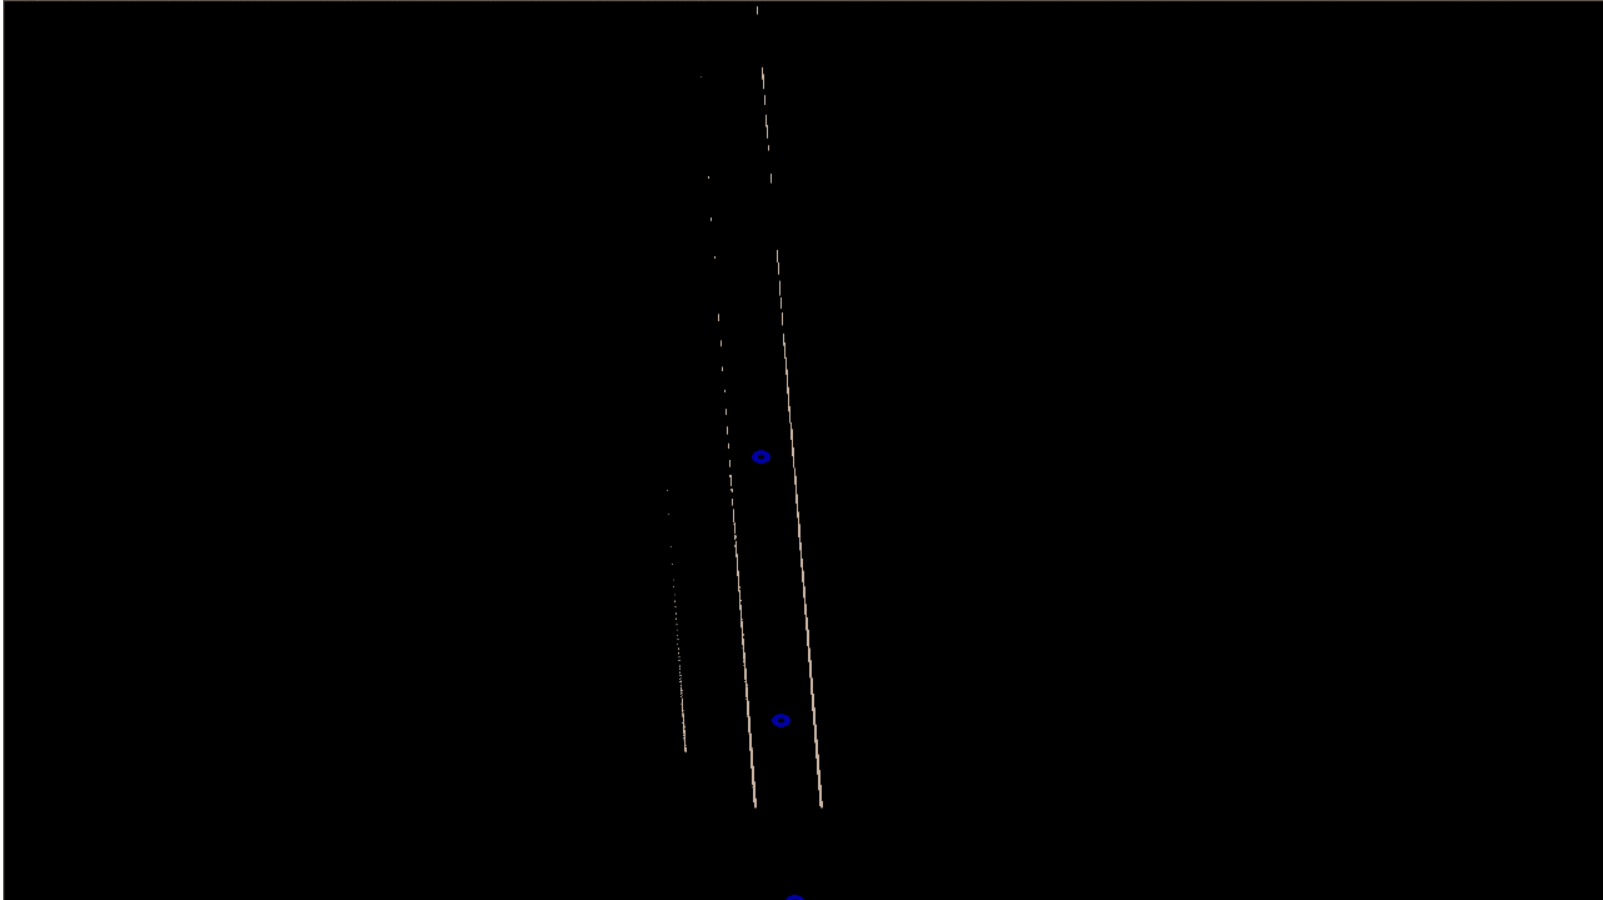
\includegraphics[width=\linewidth]{images/Waypoints.png} 
    \label{fig:lane_keep_test02_01}
\end{subfigure}\hfil
\begin{subfigure}[t]{\textwidth}
    \centering
    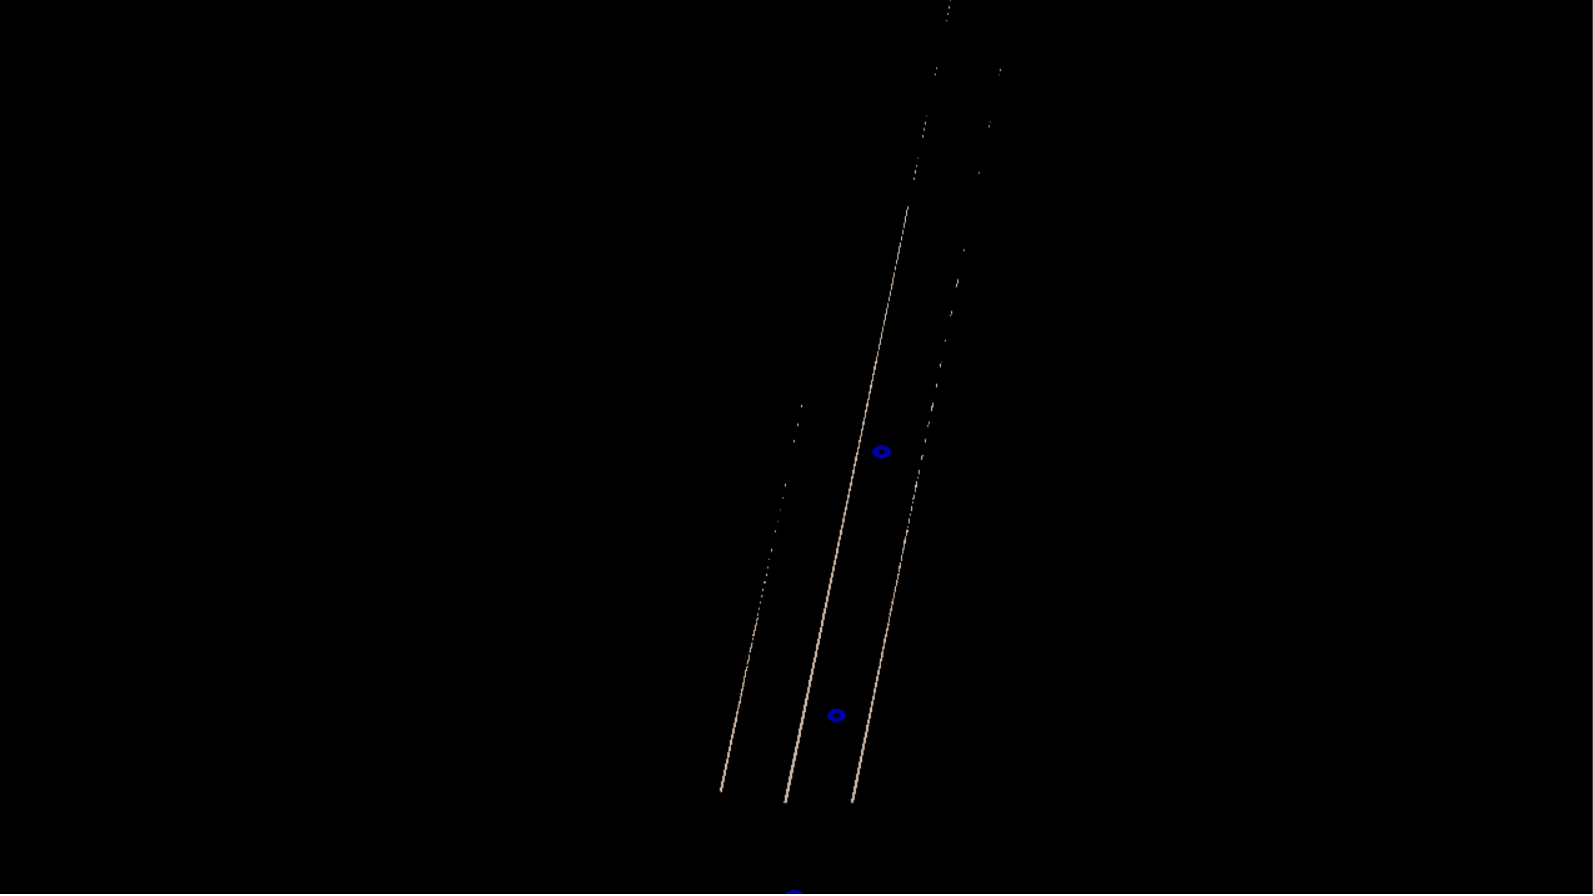
\includegraphics[width=\linewidth]{images/Waypoints02.png}
    \label{fig:lane_keep_test02_02}
\end{subfigure}\hfil

\caption{Way-points generated (in blue) appear at the center of the thresholded lane (in white) at all times in our tests. }
\label{fig:lane_keep_test02}
\end{figure}

%-----------------------------------------------------%
\subsection{Lane Changing}
\label{test_lane_change}
In order to test our lane changing module explained in \ref{method_lane_change}, test cases of many different scenarios were designed in order to show that lane changing is sometimes a feasible action while other times it is not, or even that its feasibility cannot be predicted. As mentioned in section\ref{method_lane_change}, we assume that the environment will have the ego vehicle and N vehicles surrounding it. \\
In this In this section, we assume that are only 2 vehicles in the environment; the ego vehicle and another one. The ego vehicle is the red vehicle and the yellow one is the other vehicle taking position A, B, C or D.
 We perform 6 test cases scenario. If the lane change actions tested to be infeasible; the ego vehicle doesn't move and this behaviour only appear in the lane changing module test unit. If the action was infeasible at running the whole system there is a different behaviour as it will be mentioned later.

\begin{enumerate}
     \item \textbf{Test 1:}
         \begin{itemize}
             \item \textbf{Scenario:}
             \\
             - Surrounding vehicle's position case : Case A
             \\
             - Distance between vehicles: 1.5 \(m\)
             \\
             - Ego vehicle’s starting velocity: 0.3 \(m/s\)
             \\
             - Ego vehicle’s starting position: -40 \(m\)
             \\
             - Ego vehicle’s starting lane:  Lane 1
             \\
             - Ego vehicle’s target lane:  Lane 0
             \\
             - Surrounding vehicle’s starting velocity: 0.1 \(m/s\)
             \\
             - Surrounding vehicle’s starting position: -41.5 \(m\)
             \\
             - Surrounding vehicle’s lane:  Lane 0
             \\
\begin{figure}[hbtp]
    \centering
    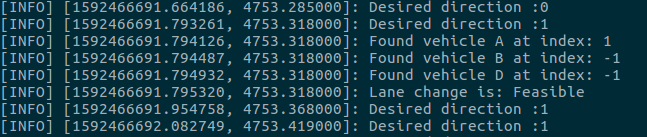
\includegraphics[width=0.75\textwidth]{images/A_F_1.5_Terminal.png}
    \caption{Lane Changing - Test 1: Case A - Terminal log - Feasible.}
    \label{fig:lane_change_T1_A_1.5_F_Terminal}
\end{figure}

\begin{figure}[hbtp]
    \centering
    \begin{subfigure}[t]{0.3\textwidth}
        \centering
        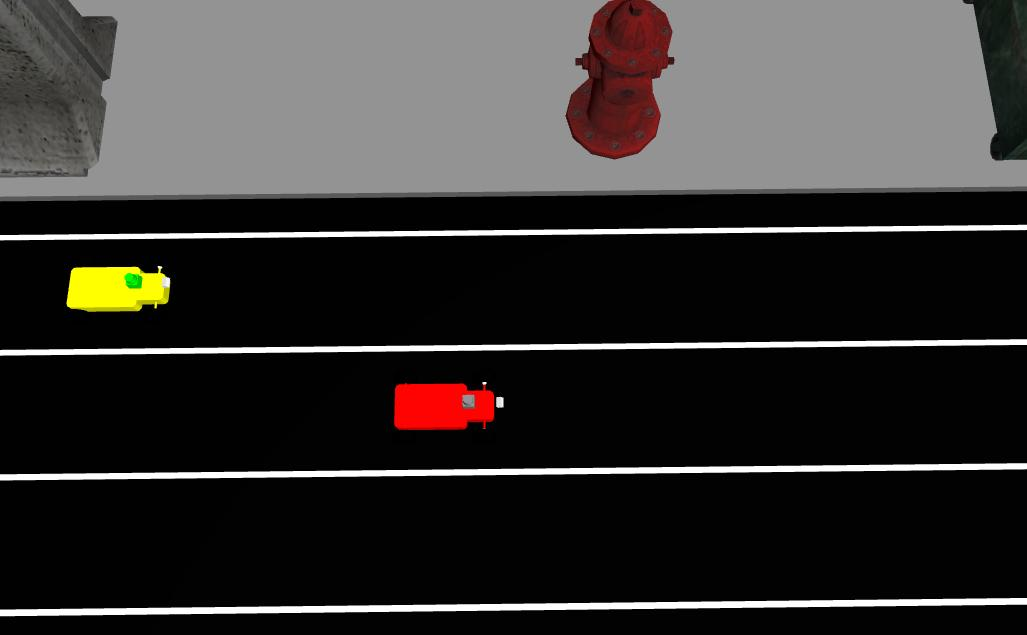
\includegraphics[width=1\linewidth, height=2.5cm]{images/A_F_1.5_1.jpg}
        \caption{Shoot 1.}
        %\label{fig:racecar_sideview}
    \end{subfigure}\hfil
    \begin{subfigure}[t]{0.3\textwidth}
        \centering
        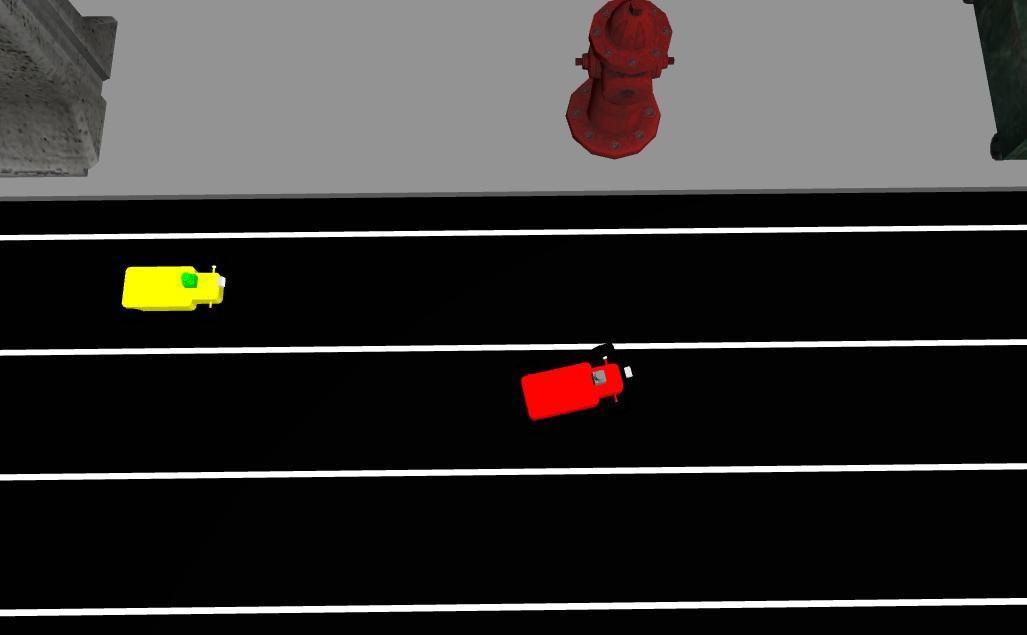
\includegraphics[width=1\linewidth, height=2.5cm]{images/A_F_1.5_2.jpg}
        \caption{Shoot 2.}
        %\label{fig:racecar_sideview}
    \end{subfigure}\hfil
    \begin{subfigure}[t]{0.3\textwidth}
        \centering
        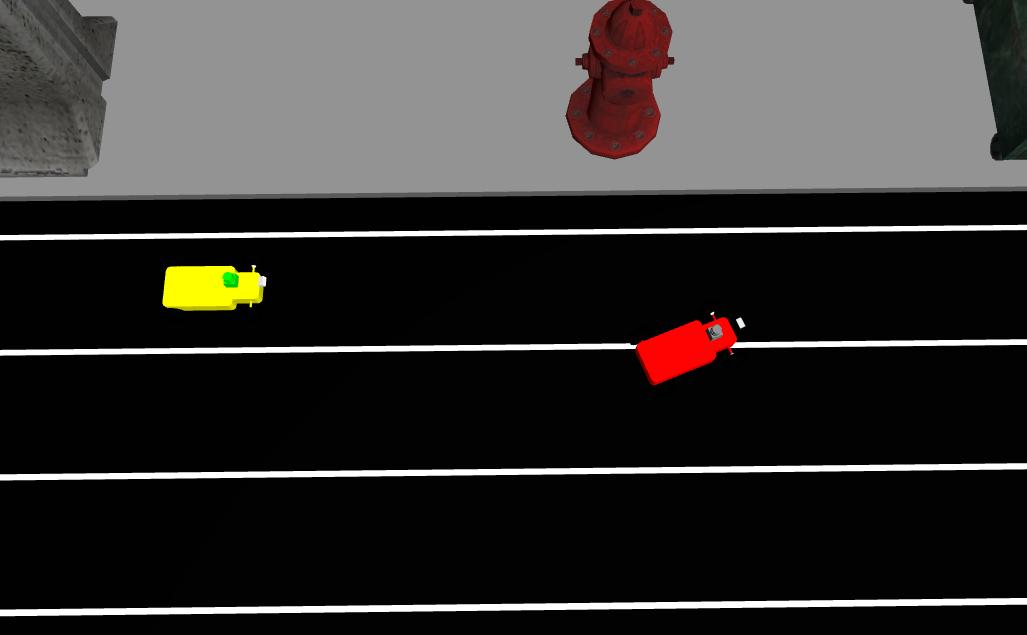
\includegraphics[width=1\linewidth, height=2.5cm]{images/A_F_1.5_3.jpg}
        \caption{Shoot 3.}
        %\label{fig:racecar_isonmetricview}
    \end{subfigure}\hfil
    \medskipd
    \begin{subfigure}[t]{0.3\textwidth}
        \centering
        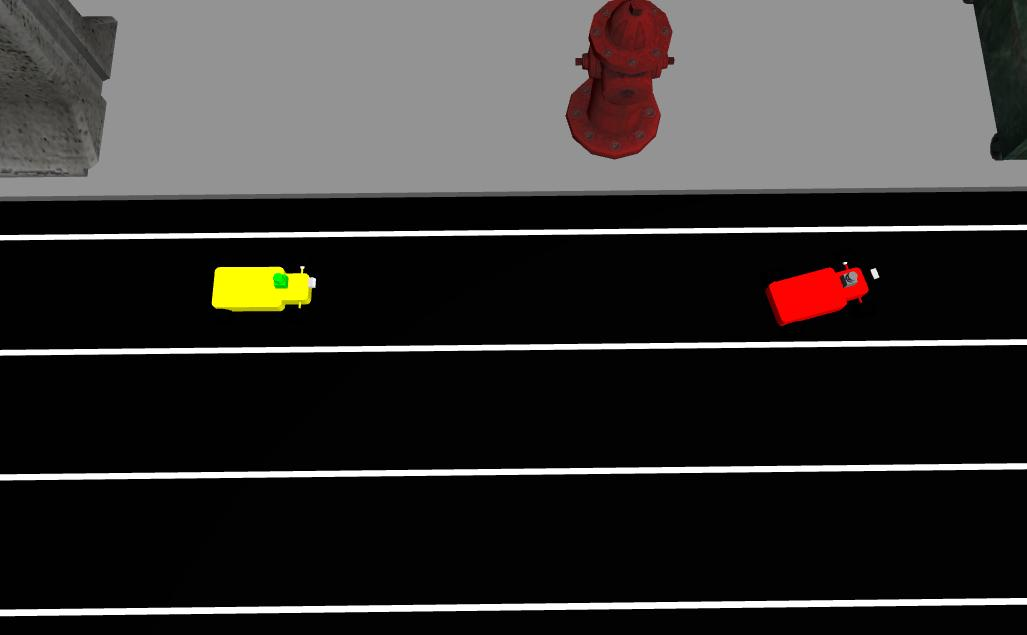
\includegraphics[width=1\linewidth, height=2.5cm]{images/A_F_1.5_4.jpg}
        \caption{Shoot 4.}
        %\label{fig:racecar_isonmetricview}
    \end{subfigure}\hfil
    \begin{subfigure}[t]{0.3\textwidth}
        \centering
        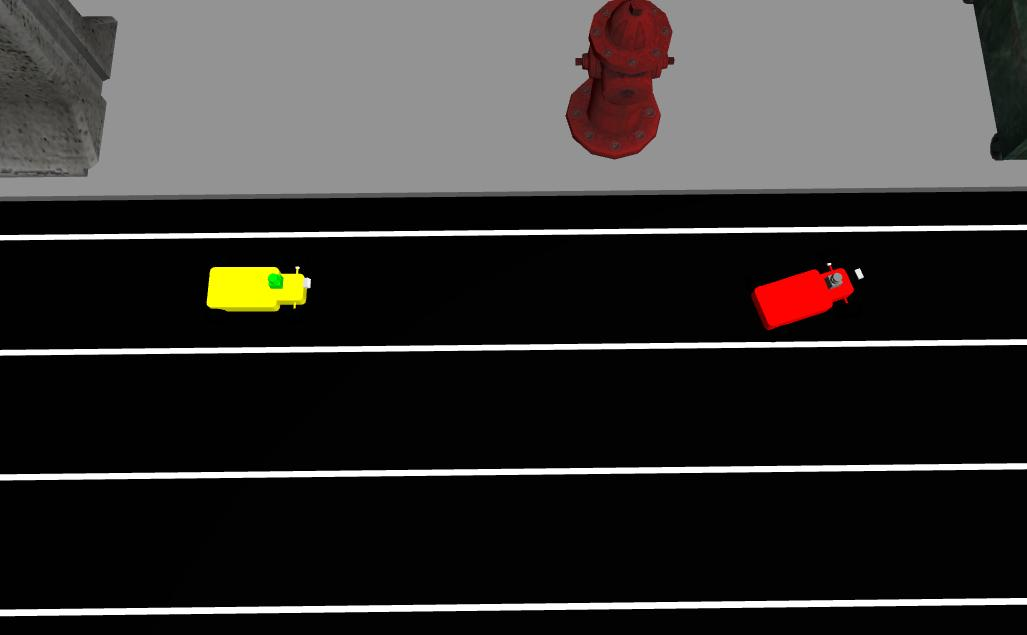
\includegraphics[width=1\linewidth, height=2.5cm]{images/A_F_1.5_5.jpg}
        \caption{Shoot 5.}
        %\label{fig:racecar_topview}
    \end{subfigure}\hfil
    \begin{subfigure}[t]{0.3\textwidth}
        \centering
        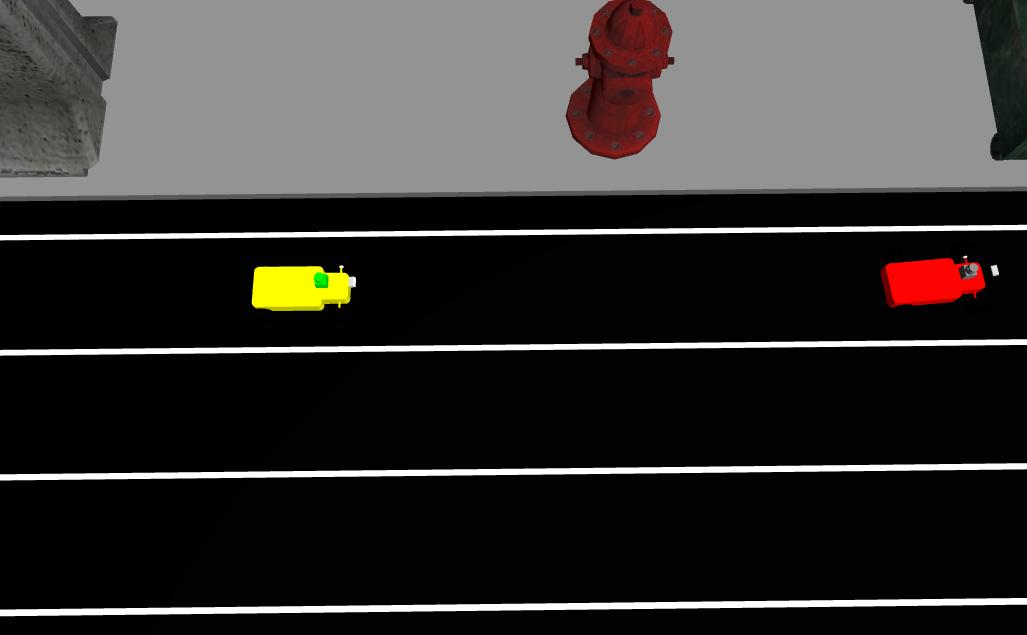
\includegraphics[width=1\linewidth, height=2.5cm]{images/A_F_1.5_6.jpg}
        \caption{Shoot 6.}
        %\label{fig:racecar_sideview}
    \end{subfigure}\hfil
    
    \caption{Lane Changing - Test 1: Case A - Feasible.}
    \label{fig:lane_change_T1_A_1.5_F}
    \end{figure}
            
             \item \textbf{Results and discussion:} \\
                       As shown in table \ref{table:lane_change_T1_A_1.5_F}, figure \ref{fig:lane_change_T1_A_1.5_F} and \ref{fig:lane_change_T1_A_1.5_F_Terminal},Vehicle at position A, the yellow vehicle, was found in the environment and lane change action checked to be feasible and will be executed. The red vehicle started from its lane and then was prompted to make a lane change action. It starts lane changing with its current velocity 0.3 \(m/s\) and the steering angle is changing throughout the time till it finishes executing the action and stops. On the other side the yellow vehicle is executing lane keeping action following Krauss model; following the red vehicle and keeping out the maximum safe velocity and distance. The results in table \ref{table:lane_change_T1_A_1.5_F} are approximate to the stated above values.\\
                       The results are logical because there is a vehicle in the ego vehicle's target lane. When the ego vehicle hypothetically reached the center-line, the yellow AV was still behind it and before the centre-line so it is in position A as expected. Also, the distance between the two vehicles was enough for the yellow vehicle to adapt its velocity following the red one.\\


 \begin{table} [hbtp]
        \begin{center}
            \begin{tabularx}{1\textwidth} { 
            | >{\centering\arraybackslash}X 
            | >{\centering\arraybackslash}X
            | >{\centering\arraybackslash}X
            | >{\centering\arraybackslash}X |}
                \hline 
                Red vehicle velocity (\(m/s\)) & Red vehicle steering angle (\(rad\)) & Yellow vehicle velocity (\(m/s\)) & Yellow vehicle steering angle (\(rad\))\\
                \hline 
                0.300000011921 & 0.0 & 0.10000000149 & 0.0\\
                \hline 
                0.300936579704 & 0.142148435116 & 0.10000000149 & 6.74655893818e-05\\
                \hline 
                0.300936579704 & -0.0928664803505 & 0.10000000149 & 0.000105529383291\\
                \hline 
                0.300936579704 & -0.0659889876842 & 0.10000000149 & 3.91086323361e-05\\
                \hline 
            \end{tabularx}
        \caption{Lane Changing velocity and steering angle throughout time - Test 1: Case A - Feasible}
        \label{table:lane_change_T1_A_1.5_F}
        \end{center}
        \end{table} 
        \end{itemize}
    \item \textbf{Test 2:}
        \begin{itemize}
             \item \textbf{Scenario:}
             \\
             - Surrounding vehicle's position case : Case A
             \\
             - Distance between vehicles: 1 \(m\)
             \\
             - Ego vehicle’s starting velocity: 0.3 \(m/s\)
             \\
             - Ego vehicle’s starting position: -40 \(m\)
             \\
             - Ego vehicle’s starting lane:  Lane 1
             \\
             - Ego vehicle’s target lane:  Lane 0
             \\
             - Surrounding vehicle’s starting velocity: 0.1 \(m/s\)
             \\
             - Surrounding vehicle’s starting position: -41 \(m\)
             \\
             - Surrounding vehicle’s lane:  Lane 0
             \\
\begin{figure}[hbtp]
    \centering
    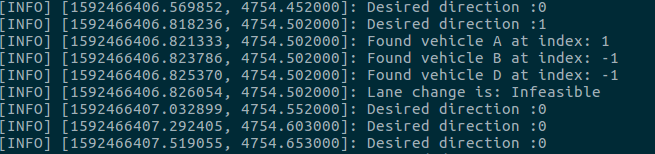
\includegraphics[width=0.75\textwidth]{images/LaneChange-Test/A_INF_1M/A_INF_1M_Terminal.png}
    \caption{Lane Changing - Test 2: Case A - Terminal log - Infeasible.}
    \label{fig:lane_change_T2_A_1M_INF_Terminal}
\end{figure}

\begin{figure}[hbtp]
    \centering
    \begin{subfigure}[t]{0.3\textwidth}
        \centering
        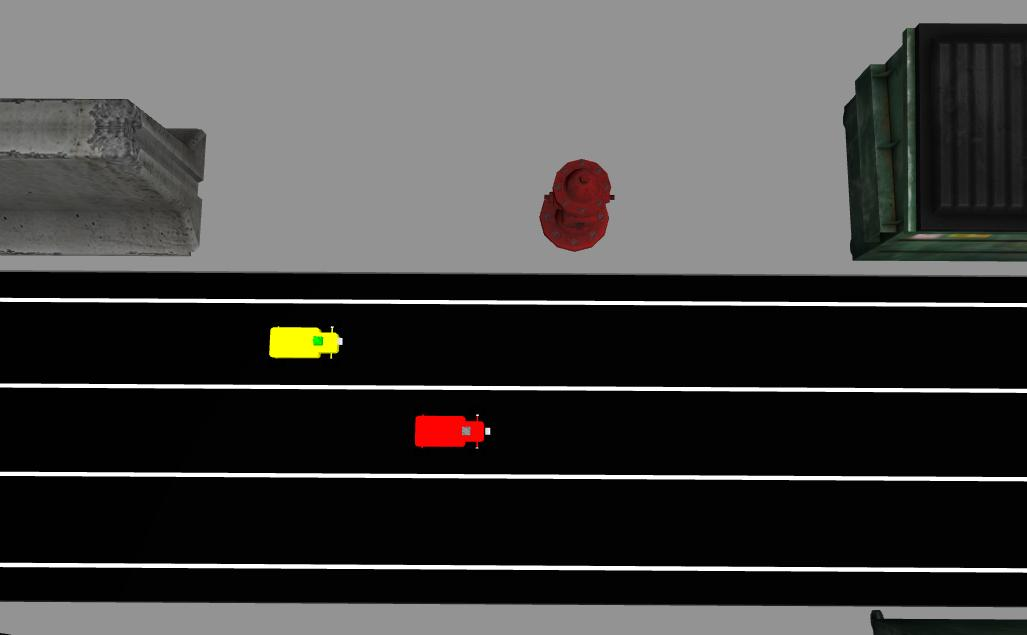
\includegraphics[width=1\linewidth, height=2.5cm]{images/LaneChange-Test/A_INF_1M/1.jpg}
        \caption{Shoot 1.}
        %\label{fig:racecar_sideview}
    \end{subfigure}\hfil
    \begin{subfigure}[t]{0.3\textwidth}
        \centering
        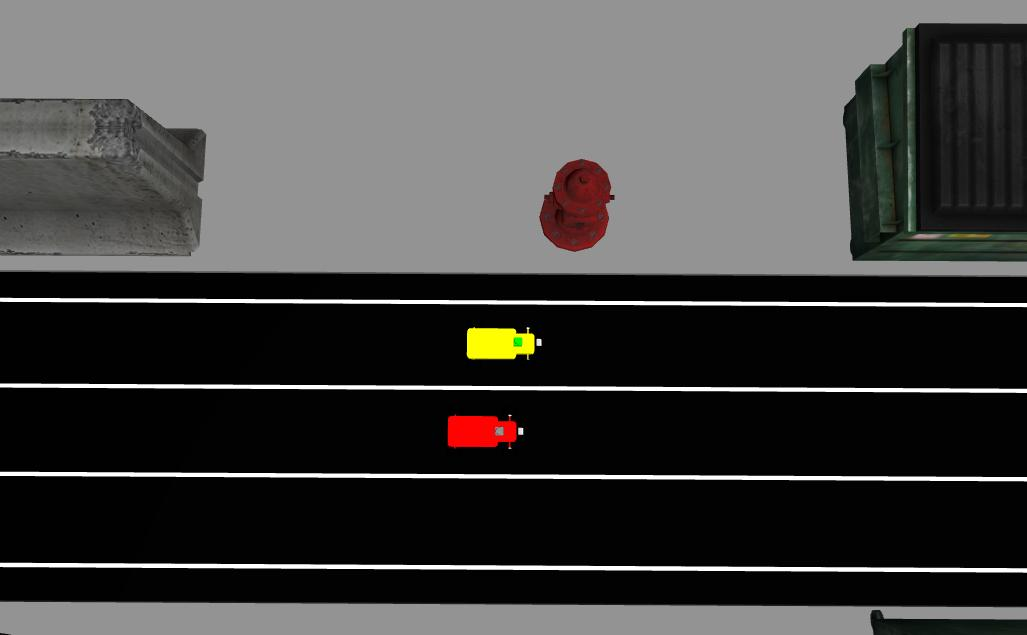
\includegraphics[width=1\linewidth, height=2.5cm]{images/LaneChange-Test/A_INF_1M/2.jpg}
        \caption{Shoot 2.}
        %\label{fig:racecar_sideview}
    \end{subfigure}\hfil
    \begin{subfigure}[t]{0.3\textwidth}
        \centering
        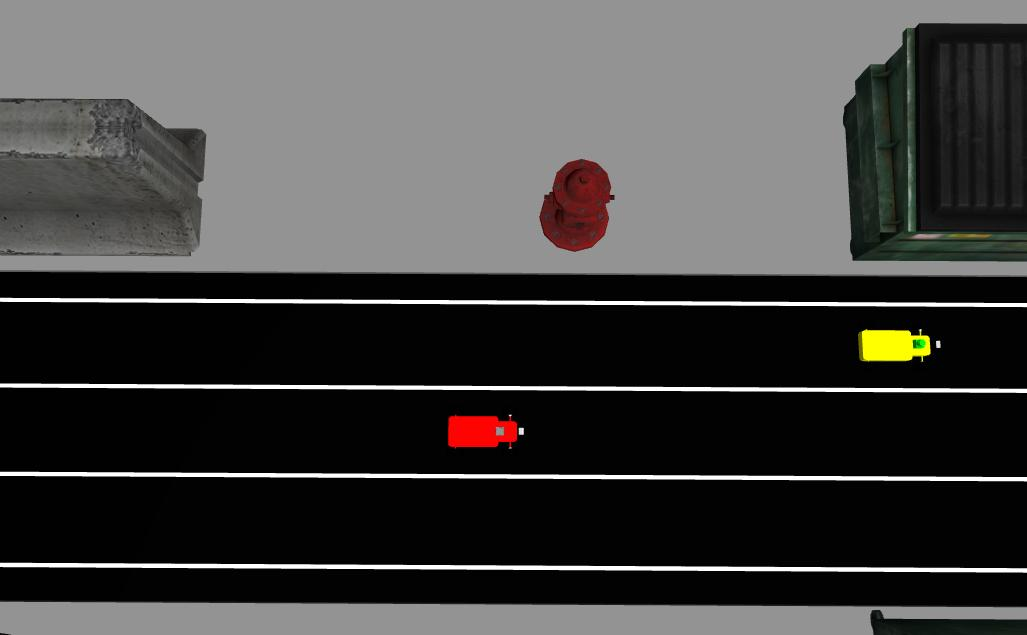
\includegraphics[width=1\linewidth, height=2.5cm]{images/LaneChange-Test/A_INF_1M/3.jpg}
        \caption{Shoot 3.}
        %\label{fig:racecar_isonmetricview}
    \end{subfigure}\hfil
 
    \caption{Lane Changing - Test 2: Case A - Infeasible}
    \label{fig:lane_change_T2_A_1M_INF}
    \end{figure}

            
             \item \textbf{Results and discussion:} \\
                       As shown in table \ref{table:lane_change_T2_A_1M_INF}, figure  \ref{fig:lane_change_T2_A_1M_INF_Terminal} and \ref{fig:lane_change_T2_A_1M_INF}, vehicle at position A was found in the environment and lane change action checked to be infeasible and will not be executed. The red vehicle's initial velocity was 0.3 \(m/s\) but it stopped as it can't perform lane change action and the yellow vehicle continues in its path. \\
                       The results are logical because there is a vehicle in the ego vehicle's target lane. When the ego vehicle hypothetically reached the center-line, the yellow AV was still behind it and before the centre-line so it is in position A as expected. However, it may be in the lane change region when the red vehicle starts to change its lane. So it returned that the lane change action is not feasible because the distance and relative velocities of the two vehicles are not enough..\\


 \begin{table} [hbtp]
        \begin{center}
            \begin{tabularx}{1\textwidth} { 
            | >{\centering\arraybackslash}X 
            | >{\centering\arraybackslash}X
            | >{\centering\arraybackslash}X
            | >{\centering\arraybackslash}X |}
                \hline 
                Red vehicle velocity (\(m/s\)) & Red vehicle steering angle (\(rad\)) & Yellow vehicle velocity (\(m/s\)) & Yellow vehicle steering angle (\(rad\))\\
                \hline 
                0.3 & 0.0 & 0.10000000149 & 0.0\\
                \hline 
                0.0 & 0.0 & 0.10000000149 & -9.10808303161e-055\\
                \hline 
                0.0 & 0.0 & 0.10000000149 & -7.47770172893e-05\\
                \hline 
                0.0 & 0.0 & 0.10000000149 & -0.000134485177114\\
                \hline 
            \end{tabularx}
        \caption{Lane Changing velocity and steering angle throughout time - Test 2: Case A - Infeasible}
        \label{table:lane_change_T2_A_1M_INF}
        \end{center}
        \end{table} 
        \end{itemize}
    \item \textbf{Test 3:}
        \begin{itemize}
             \item \textbf{Scenario:}
             \\
             - Surrounding vehicle's position case : Case Indeterminate A or B
             \\
             - Distance between vehicles: 0.5 \(m\)
             \\
             - Ego vehicle’s starting velocity: 0.3 \(m/s\)
             \\
             - Ego vehicle’s starting position: -40 \(m\)
             \\
             - Ego vehicle’s starting lane:  Lane 1
             \\
             - Ego vehicle’s target lane:  Lane 0
             \\
             - Surrounding vehicle’s starting velocity: 0.1 \(m/s\)
             \\
             - Surrounding vehicle’s starting position: -39.5 \(m\)
             \\
             - Surrounding vehicle’s lane:  Lane 0
             \\
\begin{figure}[hbtp]
    \centering
    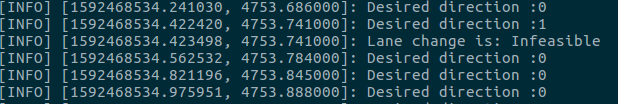
\includegraphics[width=0.75\textwidth]{images/LaneChange-Test/AorB/AorB_Terminal.png}
    \caption{Lane Changing - Test 3: Indeterminate Case A or B - Terminal log - Infeasible.}
    \label{fig:lane_change_T3_AorB_0.5_INF_Terminal}
\end{figure}

\begin{figure}[hbtp]
    \centering
    \begin{subfigure}[t]{0.3\textwidth}
        \centering
        
\includegraphics[width=1\linewidth, height=2.5cm]{images/LaneChange-Test/AorB/1.jpg}
        \caption{Shot 1.}
        %\label{fig:racecar_sideview}
    \end{subfigure}\hfil
    \begin{subfigure}[t]{0.3\textwidth}
        \centering
        
\includegraphics[width=1\linewidth, height=2.5cm]{images/LaneChange-Test/AorB/2.jpg}
        \caption{Shot 2.}
        %\label{fig:racecar_sideview}
    \end{subfigure}\hfil
    \begin{subfigure}[t]{0.3\textwidth}
        \centering
        
\includegraphics[width=1\linewidth, height=2.5cm]{images/LaneChange-Test/AorB/3.jpg}
        \caption{Shot 3.}
        %\label{fig:racecar_isonmetricview}
    \end{subfigure}\hfil
    
    \caption{Lane Changing - Test 3: Indeterminate Case A or B - Infeasible}
    \label{fig:lane_change_T3_AorB_0.5_INF}
    \end{figure}

            
             \item \textbf{Results and discussion:} \\
                       As shown in table \ref{table:lane_change_T3_AorB_0.5_INF} and figures \ref{fig:lane_change_T4_B_2_INF_Terminal}, \ref{fig:lane_change_T3_AorB_0.5_INF},the yellow vehicle seems to be at position B but this is not the case. As it is not a determined case; can't determine whether it is at position A or B because of the small gap between the two vehicles. Consequently, the algorithm returns that lane changing is not feasible according to \ref{method_lane_change}. The red vehicle's initial velocity was 0.3 \(m/s\) but it stopped at it can’t perform lane change action and the yellow vehicle continues in its path.\\
                       
 \begin{table} [htbp]
        \begin{center}
            \begin{tabularx}{1\textwidth} { 
            | >{\centering\arraybackslash}X 
            | >{\centering\arraybackslash}X
            | >{\centering\arraybackslash}X
            | >{\centering\arraybackslash}X |}
                \hline 
                Red vehicle velocity (\(m/s\)) & Red vehicle steering angle (\(rad\)) & Yellow vehicle velocity (\(m/s\)) & Yellow vehicle steering angle (\(rad\))\\
                \hline 
                0.3 & 0.0 & 0.10000000149 & 0.0\\
                \hline 
                0.0 & 0.0 & 0.10000000149 & 6.74655893818e-05\\
                \hline 
                0.0 & 0.0 & 0.10000000149 & 0.000105529383291\\
                \hline 
                0.0 & 0.0 & 0.10000000149 & 3.91086323361e-05\\
                \hline 
            \end{tabularx}
        \caption{Lane Changing velocity and steering angle throughout time - Test 3: Case Indeterminate A or B - Terminal log - Infeasible}
        \label{table:lane_change_T3_AorB_0.5_INF}
        \end{center}
        \end{table} 
        \end{itemize}
    \item \textbf{Test 4:}
        \begin{itemize}
             \item \textbf{Scenario:}
             \\
             - Surrounding vehicle's position case : Case B
             \\
             - Distance between vehicles: 2 \(m\)
             \\
             - Ego vehicle’s starting velocity: 0.3 \(m/s\)
             \\
             - Ego vehicle’s starting position: -40 \(m\)
             \\
             - Ego vehicle’s starting lane:  Lane 1
             \\
             - Ego vehicle’s target lane:  Lane 0
             \\
             - Surrounding vehicle’s starting velocity: 0.1 \(m/s\)
             \\
             - Surrounding vehicle’s starting position: -38 \(m\)
             \\
             - Surrounding vehicle’s lane:  Lane 0
             \\
\begin{figure}[htbp]
    \centering
    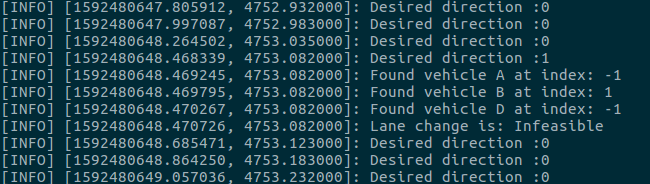
\includegraphics[width=0.75\textwidth]{images/LaneChange-Test/B_INF_2M/B_INF_2M_Terminal.png}
    \caption{Lane Changing - Test 4: Case B - Terminal log - Infeasible.}
    \label{fig:lane_change_T4_B_2_INF_Terminal}
\end{figure}

\begin{figure}[htbp]
    \centering
    \begin{subfigure}[t]{0.3\textwidth}
        \centering
        
\includegraphics[width=1\linewidth, height=2.5cm]{images/LaneChange-Test/B_INF_2M/1.jpg}
        \caption{Shot 1.}
        %\label{fig:racecar_sideview}
    \end{subfigure}\hfil
    \begin{subfigure}[t]{0.3\textwidth}
        \centering
        
\includegraphics[width=1\linewidth, height=2.5cm]{images/LaneChange-Test/B_INF_2M/2.jpg}
        \caption{Shot 2.}
        %\label{fig:racecar_sideview}
    \end{subfigure}\hfil
    \begin{subfigure}[t]{0.3\textwidth}
        \centering
        
\includegraphics[width=1\linewidth, height=2.5cm]{images/LaneChange-Test/B_INF_2M/3.jpg}
        \caption{Shot 3.}
        %\label{fig:racecar_isonmetricview}
    \end{subfigure}\hfil 
    
    \caption{Lane Changing - Test 4: Case B - Infeasible}
    \label{fig:lane_change_T4_B_2_INF}
    \end{figure}

            
             \item \textbf{Results and discussion:} \\
                       As shown in table \ref{table:lane_change_T4_B_2_INF}, figure  \ref{fig:lane_change_T4_B_2_INF_Terminal} and \ref{fig:lane_change_T4_B_2_INF}, vehicle at position B was found in the environment and lane change action checked to be infeasible and will not be executed. The red vehicle's initial velocity was 0.3 \(m/s\) but it stopped as it can't perform lane change action and the yellow vehicle continues in its path. \\
                       The results are logical because there is a vehicle in the ego vehicle's target lane. When the ego vehicle hypothetically reached the center-line, the yellow AV was ahead of the red one so it is in position B as expected. However, it may be before the right-line  when the red vehicle starts to change its lane or both the vehicles can’t maintain the minimum safe velocity between each other. So it returned that the lane change action is not feasible because the distance and relative velocities of the two vehicles are not enough.\\

 \begin{table} [htbp]
        \begin{center}
            \begin{tabularx}{1\textwidth} { 
            | >{\centering\arraybackslash}X 
            | >{\centering\arraybackslash}X
            | >{\centering\arraybackslash}X
            | >{\centering\arraybackslash}X |}
                \hline 
                Red vehicle velocity (\(m/s\)) & Red vehicle steering angle (\(rad\)) & Yellow vehicle velocity (\(m/s\)) & Yellow vehicle steering angle (\(rad\))\\
                \hline 
                0.3 & 0.0 & 0.10000000149 & 0.0\\
                \hline 
                0.0 & 0.0 & 0.10000000149 & 8.4286366473e-05\\
                \hline 
                0.0 & 0.0 & 0.10000000149 & -0.000128690691781\\
                \hline 
                0.0 & 0.0 & 0.10000000149 & -6.5345207986e-05\\
                \hline 
            \end{tabularx}
        \caption{Lane Changing velocity and steering angle throughout time - Test 4: Case B - Terminal log - Infeasible}
        \label{table:lane_change_T4_B_2_INF}
        \end{center}
        \end{table} 
        \end{itemize}
    \item \textbf{Test 5:}
        \begin{itemize}
             \item \textbf{Scenario:}
             \\
             - Surrounding vehicle's position case : Case C
             \\
             - Distance between vehicles: 1 \(m\)
             \\
             - Ego vehicle’s starting velocity: 0.3 \(m/s\)
             \\
             - Ego vehicle’s starting position: -40 \(m\)
             \\
             - Ego vehicle’s starting lane:  Lane 1
             \\
             - Ego vehicle’s target lane:  Lane 0
             \\
             - Surrounding vehicle’s starting velocity: 0.1 \(m/s\)
             \\
             - Surrounding vehicle’s starting position: -41 \(m\)
             \\
             - Surrounding vehicle’s lane:  Lane 1
             \\
\begin{figure}[htbp]
    \centering
    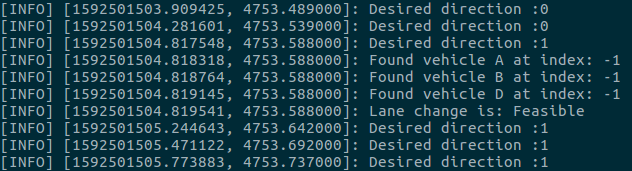
\includegraphics[width=0.75\textwidth]{images/LaneChange-Test/C_F_1/C_F_1_Terminal.png}
    \caption{Lane Changing - Test 5: Case C - Terminal log - Feasible.}
    \label{fig:lane_change_T5_C_1_F_Terminal}
\end{figure}

\begin{figure}[htbp]
     \centering
    \begin{subfigure}[t]{0.3\textwidth}
        \centering
        
\includegraphics[width=1\linewidth, height=2.5cm]{images/LaneChange-Test/C_F_1/1.jpg}
        \caption{Shot 1.}
        %\label{fig:racecar_sideview}
    \end{subfigure}\hfil
    \begin{subfigure}[t]{0.3\textwidth}
        \centering
        
\includegraphics[width=1\linewidth, height=2.5cm]{images/LaneChange-Test/C_F_1/2.jpg}
        \caption{Shot 2.}
        %\label{fig:racecar_sideview}
    \end{subfigure}\hfil
    \begin{subfigure}[t]{0.3\textwidth}
        \centering
        
\includegraphics[width=1\linewidth, height=2.5cm]{images/LaneChange-Test/C_F_1/3.jpg}
        \caption{Shot 3.}
        %\label{fig:racecar_isonmetricview}
    \end{subfigure}\hfil
    \begin{subfigure}[t]{0.3\textwidth}
        \centering
        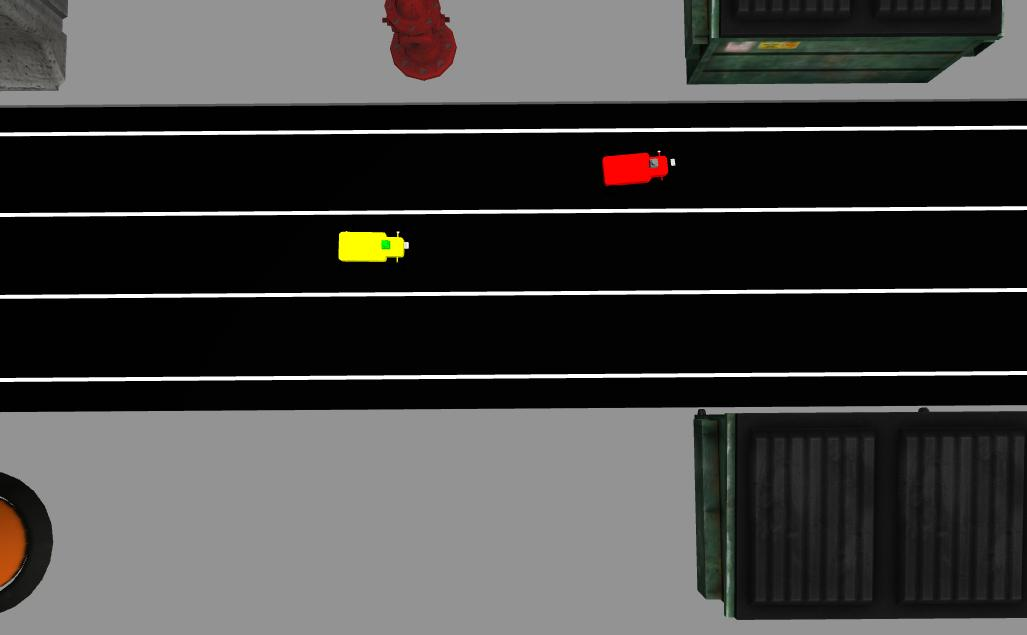
\includegraphics[width=1\linewidth, height=2.5cm]{images/LaneChange-Test/C_F_1/4.jpg}
        \caption{Shot 4.}
        %\label{fig:racecar_isonmetricview}
    \end{subfigure}\hfil
    \begin{subfigure}[t]{0.3\textwidth}
        \centering
        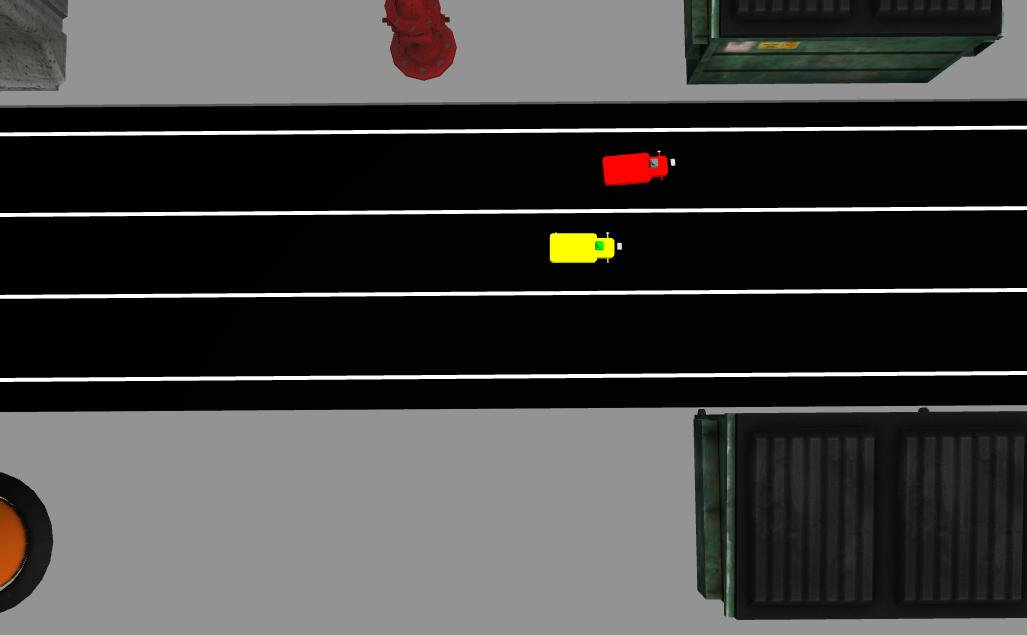
\includegraphics[width=1\linewidth, height=2.5cm]{images/LaneChange-Test/C_F_1/5.jpg}
        \caption{Shot 5.}
        %\label{fig:racecar_topview}
    \end{subfigure}\hfil
    \begin{subfigure}[t]{0.3\textwidth}
        \centering
        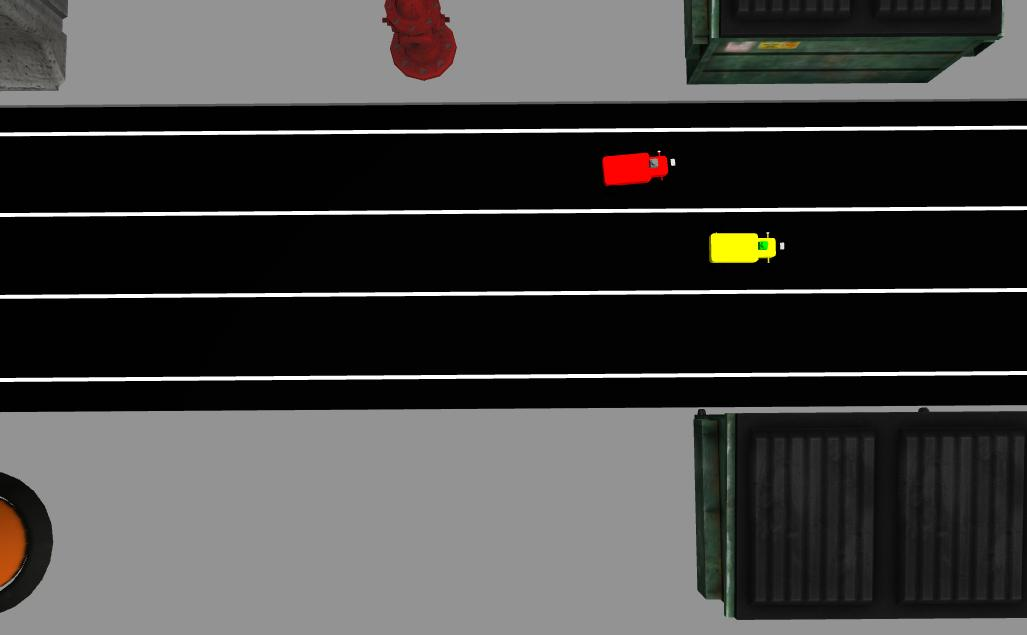
\includegraphics[width=1\linewidth, height=2.5cm]{images/LaneChange-Test/C_F_1/6.jpg}
        \caption{Shot 6.}
        %\label{fig:racecar_sideview}
    \end{subfigure}\hfil
    
    \caption{Lane Changing - Test 5: Case C - Feasible}
    \label{fig:lane_change_T5_C_1_F}
    \end{figure}

             \item \textbf{Results and discussion:} \\
                       As shown in table \ref{table:lane_change_T5_C_1_F}, figure \ref{fig:lane_change_T5_C_1_F} and \ref{fig:lane_change_T5_C_1_F_Terminal},vehicle at position C, the yellow vehicle, was found in the environment and lane change action checked to be feasible and will be executed. The red vehicle started from its lane and then was prompted to make a lane change action. It starts lane changing with its current velocity 0.3 \(m/s\) and the steering angle is changing throughout the time till it finishes executing the action and stops. On the other side the yellow vehicle is executing lane keeping action following krauss model. The results in table \ref{table:lane_change_T5_C_1_F} are approximate to the stated above values.\\
                        The results are logical because there is a vehicle in the ego vehicle's lane. The yellow vehicle is behind the red one and in the same lane; so it is at position C as expected. The yellow vehicle will not affect the lane change action by any means because it will follow the red one using krauss model at any time. When the red vehicle is outside the yellow one window or in the other lane; the yellow vehicle will increase its velocity gradually.\\



 \begin{table} [H]
        \begin{center}
            \begin{tabularx}{1\textwidth} { 
            | >{\centering\arraybackslash}X 
            | >{\centering\arraybackslash}X
            | >{\centering\arraybackslash}X
            | >{\centering\arraybackslash}X |}
                \hline 
                Red vehicle velocity (\(m/s\)) & Red vehicle steering angle (\(rad\)) & Yellow vehicle velocity (\(m/s\)) & Yellow vehicle steering angle (\(rad\))\\
                \hline 
                0.300000011921 & 0.0 & 0.10000000149 & -0.042406991124\\
                \hline 
                0.300974905491 & 0.0597243718803 & 0.10000000149 & 0.00270679476671\\
                \hline 
                0.300974905491 & 0.143652096391 & 0.10000000149 & 0.00182328152005\\
                \hline 
                0.300974905491 & -0.065448731184 & 0.10000000149 & 0.00165438361\\
                \hline 
            \end{tabularx}
        \caption{Lane Changing velocity and steering angle throughout time - Test 5: Case C - Feasible}
        \label{table:lane_change_T5_C_1_F}
        \end{center}
        \end{table} 
        \end{itemize}
    \item \textbf{Test 6:}
        \begin{itemize}
             \item \textbf{Scenario:}
             \\
             - Surrounding vehicle's position case : Case D
             \\
             - Distance between vehicles: 1 \(m\)
             \\
             - Ego vehicle’s starting velocity: 0.3 \(m/s\)
             \\
             - Ego vehicle’s starting position: -40 \(m\)
             \\
             - Ego vehicle’s starting lane:  Lane 1
             \\
             - Ego vehicle’s target lane:  Lane 0
             \\
             - Surrounding vehicle’s starting velocity: 0.1 \(m/s\)
             \\
             - Surrounding vehicle’s starting position: -39 \(m\)
             \\
             - Surrounding vehicle’s lane:  Lane 1
             \\
\begin{figure}[htbp]
    \centering
    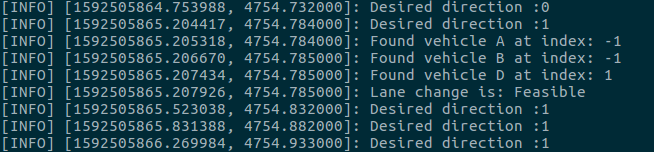
\includegraphics[width=0.75\textwidth]{images/LaneChange-Test/D_F_1/D_F_1_Terminal.png}
    \caption{Lane Changing - Test 6: Case D - Terminal log - Feasible.}
    \label{fig:lane_change_T6_D_1_F_Terminal}
\end{figure}

\begin{figure}[htbp]
    \centering
    \begin{subfigure}[t]{0.3\textwidth}
        \centering
        
\includegraphics[width=1\linewidth, height=2.5cm]{images/LaneChange-Test/D_F_1/1.jpg}
        \caption{Shot 1.}
        %\label{fig:racecar_sideview}
    \end{subfigure}\hfil
    \begin{subfigure}[t]{0.3\textwidth}
        \centering
        
\includegraphics[width=1\linewidth, height=2.5cm]{images/LaneChange-Test/D_F_1/2.jpg}
        \caption{Shot 2.}
        %\label{fig:racecar_sideview}
    \end{subfigure}\hfil
    \begin{subfigure}[t]{0.3\textwidth}
        \centering
        
\includegraphics[width=1\linewidth, height=2.5cm]{images/LaneChange-Test/D_F_1/3.jpg}
        \caption{Shot 3.}
        %\label{fig:racecar_isonmetricview}
    \end{subfigure}\hfil 
    \begin{subfigure}[t]{0.3\textwidth}
        \centering
        
\includegraphics[width=1\linewidth, height=2.5cm]{images/LaneChange-Test/D_F_1/4.jpg}
        \caption{Shot 4.}
        %\label{fig:racecar_isonmetricview}
    \end{subfigure}\hfil
    \begin{subfigure}[t]{0.3\textwidth}
        \centering
        
\includegraphics[width=1\linewidth, height=2.5cm]{images/LaneChange-Test/D_F_1/5.jpg}
        \caption{Shot 5.}
        %\label{fig:racecar_topview}
    \end{subfigure}\hfil
    \begin{subfigure}[t]{0.3\textwidth}
        \centering
        
\includegraphics[width=1\linewidth, height=2.5cm]{images/LaneChange-Test/D_F_1/6.jpg}
        \caption{Shot 6.}
        %\label{fig:racecar_sideview}
    \end{subfigure}\hfil
    
    \caption{Lane Changing - Test 6: Case D - Feasible}
    \label{fig:lane_change_T6_D_1_F}
    \end{figure}
    
             \item \textbf{Results and discussion:} \\
                       As shown in table \ref{table:lane_change_T6_D_1_F}, figure \ref{fig:lane_change_T6_D_1_F} and \ref{fig:lane_change_T6_D_1_F_Terminal},vehicle at position D, the yellow vehicle, was found in the environment and lane change action checked to be feasible and will be executed. The red vehicle started from its lane and then was prompted to make a lane change action. It starts lane changing with its current velocity 0.3 \(m/s\) and the steering angle is changing throughout the time till it finishes executing the action and stops. On the other side, the yellow vehicle is executing lane keeping action following krauss model. The results in table \ref{table:lane_change_T6_D_1_F} are approximate to the stated above values.\\
                       The results are logical because there is a vehicle in the ego vehicle's lane. The yellow vehicle is in front of  the red one and in the same lane; so it is at position D as expected. If the yellow vehicle stops or performs maximum deceleration all the time steps that the red vehicle takes to reach the centerline its position will be after the centerline; so it is a feasible lane change action. Moreover, the yellow vehicle will continue its path and will not be affected by the red vehicle at all and its velocity will increase gradually.\\

 \begin{table} [htbp]
        \begin{center}
            \begin{tabularx}{1\textwidth} { 
            | >{\centering\arraybackslash}X 
            | >{\centering\arraybackslash}X
            | >{\centering\arraybackslash}X
            | >{\centering\arraybackslash}X |}
                \hline 
                Red vehicle velocity (\(m/s\)) & Red vehicle steering angle (\(rad\)) & Yellow vehicle velocity (\(m/s\)) & Yellow vehicle steering angle (\(rad\))\\
                \hline 
                0.300000011921 & 0.0 & 0.10000000149 & -0.042406991124\\
                \hline 
                0.272501945496 & 0.0689768791199 & 0.10000000149 & 6.0399153881e-05\\
                \hline 
                0.272501945496 & -0.111118324101 & 0.10000000149 & -7.31826658011e-05\\
                \hline 
                0.272501945496 & -0.0656164810061 & 0.10000000149 & -8.78940845723e-05\\
                \hline 
            \end{tabularx}
        \caption{Lane Changing velocity and steering angle throughout time - Test 6: Case D - Feasible}
        \label{table:lane_change_T6_D_1_F}
        \end{center}
        \end{table} 
        \end{itemize}
\end{enumerate}
%-----------------------------------------------------%
\subsection{Path Planning}
\label{test_path_plan}
In this sub-section, we test our two main additions, explained in \ref{method_path_plan}, to the path planning module.

\begin{itemize}
    \item \textbf{Communication Layer Testing:} 
    \\ \\
    In order to test the different functionalities that our communication costmap layer ought to be able to perform, we designed three tests. The aim of the first is to validate that our costmap layer is able to clear and mark cells as expected when being used as a layer of either the global costmap, used by the global planner to generate the global path, or the local layered costmap, used by the local planner to generate the local path. Hence, our ego vehicle and one another are placed such that they are both inside each other’s communication range, and then the other vehicle is allowed to move. The expected result of this test is that our vehicle manages to mark the footprint of the other at all times, and clear the cells which were previously marked but are now free. 
    \\ \\
    The aim of the second test is to make sure that the global planner does take into consideration the cells marked as LETHAL by our communication layer when added to the global costmap, but not the local one. Thus, our vehicle is given a goal to which it is allowed to navigate in the presence of the other vehicle. The global path generated by the global planner as well as our vehicle’s motion are to be observed. It is expected that the global path does not pass through any of the marked cells within the footprint of the other vehicle. 
    \\ \\
    For the third test, we verify that the local planner considers the cells marked as LETHAL by our costmap layer when it is added to the local costmap but not the global costmap.. Again, our vehicle is given the same task of navigating  to goal in the presence of the other vehicle. The expected result is that, regardless of the global path generated by the global planner, the local planner forces our vehicle to avoid any marked cells within the other vehicle’s footprint. 
    \\ \\
    For all the tests, in order to be able to display the output of the communication layer, the vehicles’ LiDAR sensors were raised a little above the vehicle bodies so the bodies are not detected by the sensors, and hence not displayed in the obstacle layer of the costmaps. To demonstrate the results of all three tests, figures of the vehicles’ top-view in the different costmaps are shown in RViz, a 3D visualizer of environments, robots and sensor data \cite{RVizarticle}.
    
    \begin{enumerate}
        \item \textbf{Test 1:}
            \begin{itemize}
                \item \textbf{Scenario:}
                \begin{itemize}
                    \item Global costmap layers in order:
                \begin{enumerate}
                    \item Static Layer
                    \item Obstacle Layer
                    \item Communication Layer
                    \item Inflation Layer
                \end{enumerate}
                    \item Local costmap layers in order:
                \begin{enumerate}
                    \item Static Layer
                    \item Obstacle Layer
                    \item Communication Layer
                \end{enumerate}
                    \item Ego vehicle’s starting position: in the right-most lane at an x-coordinate of -0.5 m (shown in red in figures \ref{comm_test1_G} and \ref{comm_test1_L})
                    \item Other vehicle’s starting position: in the middle lane at an x-coordinate of 0.5 m (shown in yellow in figures \ref{comm_test1_G} and \ref{comm_test1_L})
                \end{itemize}

                \item \textbf{Results and discussion:} \\
                As shown in figures \ref{fig:costmap_T1G1_fig} and \ref{fig:costmap_T1L1_fig} of the global and local costmaps of our red ego vehicle, the footprint of the other vehicle was successfully marked as LETHAL in both costmaps. The yellow vehicle was then given a goal, indicated by RViz as an arrow, and thus allowed to move towards the goal. All while the vehicle was moving, the cells marked as LETHAL in both costmaps moved along with it, indicating successful clearing and marking of the free and occupied cells respectively as shown in figures \ref{fig:costmap_T1G2_fig} and \ref{fig:costmap_T1L2_fig}. Lastly, the yellow vehicle was given another goal which lies outside the bounds of the local costmap. As expected, the footprint was marked in the global costmap but not seen by the local costmap, as shown in figures \ref{fig:costmap_T1G3_fig} and \ref{fig:costmap_T1L3_fig}.
                
    \begin{figure}[htbp]
    \centering
    \begin{subfigure}[t]{0.3\textwidth}
        \centering
        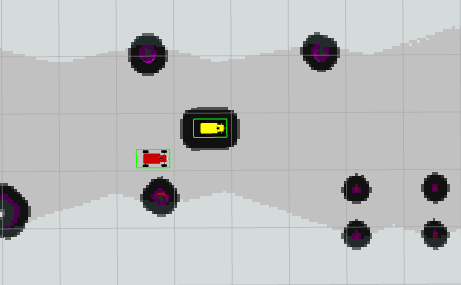
\includegraphics[width=1\linewidth, height=2.5cm]{images/costmap_T1G1.png}
        \caption{Initial position of vehicles.}
        \label{fig:costmap_T1G1_fig}
    \end{subfigure}\hfil
    \begin{subfigure}[t]{0.3\textwidth}
        \centering
        
\includegraphics[width=1\linewidth, height=2.5cm]{costmap_T1G2}
        \caption{Appropriate clearing and marking of cells while yellow vehicle is moving.}
        \label{fig:costmap_T1G2_fig}
    \end{subfigure}\hfil
    \begin{subfigure}[t]{0.3\textwidth}
        \centering
        
\includegraphics[width=1\linewidth, height=2.5cm]{costmap_T1G3}
        \caption{Marked footprint is still moving with the yellow vehicle till its goal.}
        \label{fig:costmap_T1G3_fig}
    \end{subfigure}\hfil
    
    \caption{Communication Layer - Test 1: Ego (red) vehicle's global costmap (RViz).}
    \label{comm_test1_G}
    \end{figure}

    \begin{figure}[hbtp]
    \centering
    \begin{subfigure}[t]{0.3\textwidth}
        \centering
        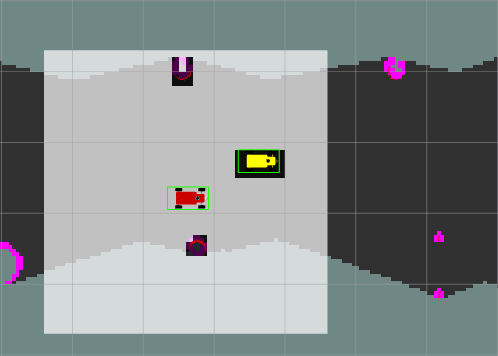
\includegraphics[width=1\linewidth, height=2.5cm]{images/costmap_T1L1.png}
        \caption{Initial position of vehicles.}
        \label{fig:costmap_T1L1_fig}
    \end{subfigure}\hfil
    \begin{subfigure}[t]{0.3\textwidth}
        \centering
        
\includegraphics[width=1\linewidth, height=2.5cm]{costmap_T1L2}
        \caption{Appropriate clearing and marking of cells while yellow vehicle is moving.}
        \label{fig:costmap_T1L2_fig}
    \end{subfigure}\hfil
    \begin{subfigure}[t]{0.3\textwidth}
        \centering
        
\includegraphics[width=1\linewidth, height=2.5cm]{costmap_T1L3}
        \caption{Yellow vehicle is outside the bounds of the local costmap.}
        \label{fig:costmap_T1L3_fig}
    \end{subfigure}\hfil
    
    \caption{Communication Layer - Test 1: Ego (red) vehicle's local costmap (RViz).}
    \label{comm_test1_L}
    \end{figure}
    
            \end{itemize}

        \item \textbf{Test 2:}
            \begin{itemize}
                \item \textbf{Scenario:}
                \begin{itemize}
                    \item Global costmap layers in order:
                \begin{enumerate}
                    \item Static Layer
                    \item Obstacle Layer
                    \item Communication Layer
                    \item Inflation Layer
                \end{enumerate}
                    \item Local costmap layers in order:
                \begin{enumerate}
                    \item Static Layer
                    \item Obstacle Layer
                \end{enumerate}
                    \item Both vehicles started at the same initial positions as those of test 1 and with the same color convention.
                \end{itemize}
                \item \textbf{Results and discussion:} \\
                Since the communication layer was only added to the ego vehicle’s global costmap but not its local costmap, the other vehicle’s footprint only appeared in the global costmap, as evident in figure \ref{comm_test2_GL}. When our ego vehicle was given a goal in front of the yellow vehicle, the generated global path took the other vehicle’s footprint into consideration and planned a path that is outside its bounds. This is shown in figure \ref{comm_test2_G}, where the arrow indicates the position of the goal and the drawn line indicates the generated global path. This coincides with the expected results since the global planner uses the global costmap in generating the path. Consequently, given that the global costmap marked the other vehicle’s footprint as LETHAL, the global planner is aware of its existence and planned the path accordingly.
                
    \begin{figure}[hbtp]
    \centering
    \begin{subfigure}[t]{0.4\textwidth}
        \centering
        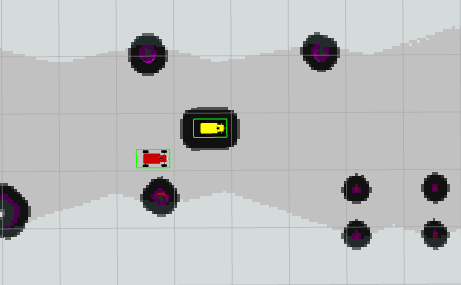
\includegraphics[width=1\linewidth, height=4cm]{images/costmap_T2G.png}
        \caption{Yellow vehicle's footprint marked in the global costmap.}
        \label{fig:costmap_T2G_fig}\hfil
    \end{subfigure}
    \begin{subfigure}[t]{0.4\textwidth}
        \centering
        
\includegraphics[width=1\linewidth, height=4cm]{costmap_T2L}
        \caption{Yellow vehicle's footprint not marked in the local costmap.}
        \label{fig:costmap_T2L_fig}\hfil
    \end{subfigure}
    \caption{Communication Layer - Test 2: Communication layer added only to the ego (red) vehicle's global costmap (RViz).}
    \label{comm_test2_GL}
    \end{figure}

    \begin{figure}[hbtp]
    \centering
    \begin{subfigure}[t]{0.3\textwidth}
    \centering
        
\includegraphics[width=1\linewidth, height=2.5cm]{costmap_T2G1.png}
        \caption{Generated global path avoids yellow vehicle's footprint.}
        \label{fig:costmap_T2G1_fig}
    \end{subfigure}\hfil
    \begin{subfigure}[t]{0.3\textwidth}
        \centering
        
\includegraphics[width=1\linewidth, height=2.5cm]{costmap_T2G2}
        \caption{Ego vehicle navigates to the goal following the global path.}
        \label{fig:costmap_T1L2_fig}
    \end{subfigure}\hfil
    \begin{subfigure}[t]{0.3\textwidth}
        \centering
        
\includegraphics[width=1\linewidth, height=2.5cm]{costmap_T2G3.png}
        \caption{Ego vehicle reaches goal.\\}
        \label{fig:costmap_T1L3_fig}
    \end{subfigure}\hfil
    \caption{Communication Layer - Test 2: Ego (red) vehicle's global costmap while navigating to goal (RViz).}
    \label{comm_test2_G}
    \end{figure}
                
            \end{itemize}
        \item \textbf{Test 3:}
            \begin{itemize}
                \item \textbf{Scenario:}
                \begin{itemize}
                    \item Global costmap layers in order:
                \begin{enumerate}
                    \item Static Layer
                    \item Obstacle Layer
                    \item Inflation Layer
                \end{enumerate}
                    \item Local costmap layers in order:
                \begin{enumerate}
                    \item Static Layer
                    \item Obstacle Layer
                    \item Communication Layer
                \end{enumerate}
                    \item Both vehicles started at the same initial positions as those of test 1 and with the same color convention.
                \end{itemize}
                \item \textbf{Results and discussion:} \\
                In this test, the communication layer was added to the ego vehicle’s local costmap but not its global one. As a result, the other vehicle’s footprint only appeared in the local costmap, as shown in figure \ref{comm_test3_GL}. When the same goal as that in test 2 was given to our ego vehicle, the global planner generated a path that passed through the yellow vehicle’s footprint. This makes sense since the communication layer is not a part of the global costmap, hence according to the global planner, these cells are free. \\ 
                
                After the generation of the global path, the vehicle started to move towards the goal. However, the vehicle did not follow this generated global path and took a longer one which did not cross the yellow vehicle's footprint, as depicted in figure \ref{comm_test3_L}. This behavior matches the expected since the communication layer was a part of the local costmap. Therefrom, the local planner was aware of the presence of the yellow vehicle as its footprint was marked as LETHAL; hence it generated a local path for the ego vehicle to follow such that it did not collide with the yellow vehicle but managed to stick to the global path as much as possible, and eventually reached the goal.

    \begin{figure}[H]
    \centering
    \begin{subfigure}[t]{0.45\textwidth}
        \centering
        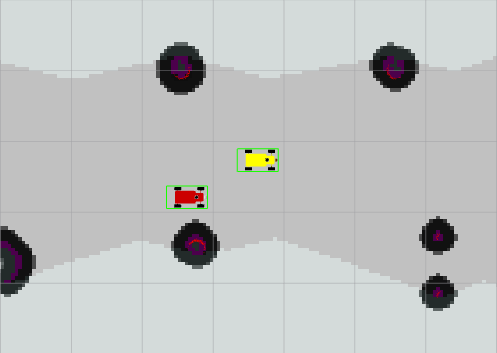
\includegraphics[width=1\linewidth, height=4cm]{images/costmap_T3G.png}
        \caption{Yellow vehicle's footprint not marked in the global costmap.}
        \label{fig:costmap_T3G_fig}
    \end{subfigure}\hfil
    \begin{subfigure}[t]{0.45\textwidth}
        \centering
        
\includegraphics[width=1\linewidth, height=4cm]{costmap_T3L}
        \caption{Yellow vehicle's footprint marked in the local costmap.}
        \label{fig:costmap_T3L_fig}
    \end{subfigure}\hfil
    \caption{Communication Layer - Test 3: Communication layer added only to the ego (red) vehicle's local costmap (RViz).}
    \label{comm_test3_GL}
    \end{figure}

    \begin{figure}[H]
    \centering
    \begin{subfigure}[t]{0.3\textwidth}
        \centering
        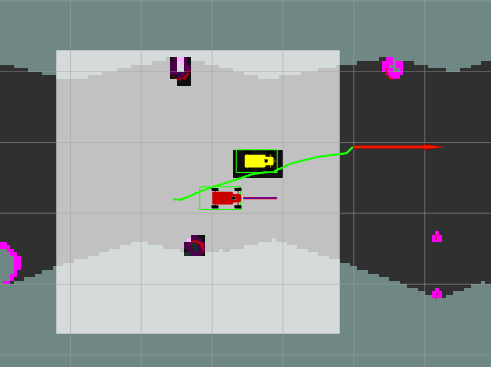
\includegraphics[width=1\linewidth, height=2.5cm]{images/costmap_T3L1.png}
        \caption{Generated global path does not avoid yellow vehicle's footprint.}
        \label{fig:costmap_T3L1_fig}
    \end{subfigure}\hfil
    \begin{subfigure}[t]{0.3\textwidth}
        \centering
        
\includegraphics[width=1\linewidth, height=2.5cm]{costmap_T3L2}
        \caption{Ego vehicle deviates from the global path to avoid yellow vehicle.}
        \label{fig:costmap_T3L2_fig}
    \end{subfigure}\hfil
    \begin{subfigure}[t]{0.3\textwidth}
        \centering
        
\includegraphics[width=1\linewidth, height=2.5cm]{costmap_T3L3}
        \caption{Ego vehicle reaches goal.\\}
        \label{fig:costmap_T3L3_fig}
    \end{subfigure}\hfil
    \caption{Communication Layer - Test 3: Ego (red) vehicle's local costmap while navigating to goal (RViz).}
    \label{comm_test3_L}
    \end{figure}

            \end{itemize}
    \end{enumerate}
    
    \item \textbf{Custom Lane Planner Testing:}
    In order for the local planner to be verified, all control actions have to be tested in all lanes. We checked seven test cases in table \ref{table:path_test_scn_res}. The table contains the cases and the chosen action in each one. 
        \begin{table} [H]
        \centering
            \begin{tabularx}{1.1\textwidth} { 
            | >{\centering\arraybackslash}X 
            | >{\centering\arraybackslash}X 
            | >{\centering\arraybackslash}X 
            | >{\centering\arraybackslash}X
            | >{\centering\arraybackslash}X
            | >{\centering\arraybackslash}X| }
                \hline 
                Number & Current (y-position) & Current Lane Number & Goal (y-position) & Future Lane Number & Chosen Action\\
                \hline 
                1 & 0.2625 & 0 & 0.2914 & 0 & Lane Keeping\\
                \hline
                2 & 0.2625 & 0 & -0.3502 & 1 & Right Lane Changing\\ 
                \hline
                3 &-0.2625 & 1 & -0.2641 & 1 & Lane Keeping\\
                \hline
                4 & -0.2625 & 1 & 0.4311 & 0 & Left Lane Changing\\
                \hline
                5 & -0.2625 & 1 & -1.102 & 2 & Right Lane Changing\\
                \hline
                6 & -0.75 & 2 & -0.7786 & 2 & Lane Keeping\\
                \hline
                7 & -0.75 & 2 & 0.7725 & 1 & Left Lane Changing\\
                \hline
            \end{tabularx}
            
        \caption{Path Planning - Test Cases: Scenarios and Results}
        \label{table:path_test_scn_res}
        \end{table} 
 
        \begin{figure}[H]
        \centering
            \begin{subfigure}[t]{0.27\textwidth}
                \centering
                
\includegraphics[width=1\linewidth]{Path1} 
                \caption{Test 1}
                \label{fig:Path1}
            \end{subfigure}\hfil
            %\hspace{0.5cm}
            \begin{subfigure}[t]{0.27\textwidth}
                \centering
                
\includegraphics[width=1\linewidth]{Path2} 
                \caption{Test 2}
                \label{fig:Path2}
            \end{subfigure}\hfil
            %\hspace{0.5cm}
            \begin{subfigure}[t]{0.27\textwidth}
                \centering
                
\includegraphics[width=1\linewidth]{Path3} 
                \caption{Test 3}
                \label{fig:Path3}
            \end{subfigure}\hfil
            %\hspace{0.5cm}
            \begin{subfigure}[t]{0.27\textwidth}
                \centering
                
\includegraphics[width=1\linewidth]{Path4} 
                \caption{Test 4}
                \label{fig:Path4}
            \end{subfigure}\hfil
            %\hspace{0.5cm}
            \begin{subfigure}[t]{0.27\textwidth}
                \centering
                
\includegraphics[width=1\linewidth]{Path5} 
                \caption{Test 5}
                \label{fig:Path5}
            \end{subfigure}\hfil
            %\hspace{0.5cm}
            \begin{subfigure}[t]{0.27\textwidth}
                \centering
                
\includegraphics[width=1\linewidth]{Path6} 
                \caption{Test 6}
                \label{fig:Path6}
            \end{subfigure}\hfil
            %\hspace{0.5cm}
            \begin{subfigure}[t]{0.27\textwidth}
                \centering
                
\includegraphics[width=1\linewidth]{Path7} 
                \caption{Test 7}
                \label{fig:Path7}
            \end{subfigure}\hfil
            \caption{Test Cases and Results}
            \label{fig:PathPlanner}
            \end{figure}
    
\end{itemize}

%-----------------------------------------------------%


%-----------------------------------------------------%
%-----------------------------------------------------%
%-----------------------------------------------------%
%-----------------------------------------------------%
\subsection{Navigation}
In order to test the navigation module discussed in \ref{method_nav}, we to verify that all AVs in the same environment drive towards their goals, do the essential maneuvers to avoid accidents and obstacles, either do lane keeping or lane changing, and stop when they reach their destinations. Therefore, we designed two test cases to measure how well the system is integrated in a smooth way through the following:
\begin{enumerate}
    \item \textbf{Test 1:}\label{NavTest1P} It includes only one AV in a static environment, uses global and local costmaps. It checks if the AV:
    \begin{enumerate}
        \item \label{NavTest1P1}Make good path plans. 
        \item \label{NavTest1P2}Goes to multiple destinations in different lanes.
        \item \label{NavTest1P3}Only does lane keeping and lane changing.
        \item \label{NavTest1P4}Stops at the closest distance to the goal. 
        \item \label{NavTest1P5}Does not make redundant maneuvers. 
        \item \label{NavTest1P6}Does not hit any static obstacle. 
        \item \label{NavTest1P7}Does not stop unless it reaches the goal or get stuck. 
    \end{enumerate}
    \item \textbf{Test 2:}\label{NavTest2P} It includes two moving AVs, therefore, the environment becomes dynamic and uses global, local, and communication costmaps. It checks if the AVs can do the previous checks in test 1 beside: 
    \begin{enumerate}
        \item \label{NavTest2P1}Don't make accidents with each other or with the surroundings (Do accurate feasibility checks)
        \item \label{NavTest2P2}Use information communicated through v2v to make accurate lane keeping and lane changing.
    \end{enumerate}
\end{enumerate}

\label{test_nav}
\begin{enumerate}
    \item \textbf{Test 1:} 
    
    \begin{itemize}
        \item \textbf{Scenario:} The scenario includes four goals that requires unique control actions to reach them.
    \end{itemize}
    
    \begin{table} [H]
        \centering
        \begin{tabularx}{1\textwidth} { 
        | >{\centering\arraybackslash}X 
        | >{\centering\arraybackslash}X 
        | >{\centering\arraybackslash}X 
        | >{\centering\arraybackslash}X| }
            \hline 
            Type & x-position (m) & y-position (m) & Lane Number\\
            \hline 
            Starting Position & -50.00 & -0.2625 & 1\\
            \hline 
            First Goal & -45.21 & -0.2661 & 1\\
            \hline 
            Second Goal & -39.13 & -1.263 & 2\\
            \hline 
            Third Goal & -30.54 & 0.2634 & 0\\
            \hline 
            Fourth Goal & -24.26 & -0.1573 & 1\\
            \hline
        \end{tabularx}
    \caption{Navigation - Test 1: Scenario}
    \label{table:nav_test1_scn}
    \end{table} 
    
    \begin{itemize}
        \item \textbf{Results and discussion:}
         \begin{table} [H]
        \centering
        \begin{tabularx}{1\textwidth} { 
        | >{\centering\arraybackslash}X 
        | >{\centering\arraybackslash}X 
        | >{\centering\arraybackslash}X 
        | >{\centering\arraybackslash}X| }
            \hline 
            Goal Number & x-position (m) & y-position (m) & Lane Number\\
            \hline 
            First Goal & -44.01 & -0.2624 & 1\\
            \hline 
            Second Goal & -37.35 & -0.7556 & 2\\
            \hline 
            Third Goal & -28.08 & 0.1662 & 0\\
            \hline 
            Fourth Goal & -20.80 & -0.2342 & 1\\
            \hline
            \end{tabularx}
            \caption{Navigation - Test 1: Results}
            \label{table:nav_test1_results}
        \end{table}
    
    
        \begin{table} [H]
        \centering
        \begin{tabularx}{1\textwidth} { 
        | >{\centering\arraybackslash}X 
        | >{\centering\arraybackslash}X 
        | >{\centering\arraybackslash}X |}
            \hline 
            Goal Number & Error x-position (m) & Error in Lane Number\\
            \hline 
            First Goal & -1.20 & 0\\
            \hline 
            Second Goal & -1.78 & 0\\
            \hline 
            Third Goal & -2.46 & 0\\
            \hline 
            Fourth Goal & -3.46 & 0\\
            \hline
        \end{tabularx}
        \caption{Navigation - Test 1: Error between planned goals and actual destinations}
        \label{table:nav_test1_results_errors}
        \end{table} 
    
        According to tables \ref{table:nav_test1_results} and \ref{table:nav_test1_results_errors}, the AV always reached the desired lane number; however, a relatively large error is observed in the goals' results (actual destinations). There are two reasons accounting for this error:
        \begin{enumerate}
            \item The frequency of the local planner in the path planning module (\ref{method_path_plan}) is much higher than the frequency of system controls, either longitudinal control (\ref{method_long_ctrl}) or lateral control (\ref{method_lat_ctrl}). \\ To illustrate, consider the following example: 
            \\ \\
            If the AV wants to use its maximum acceleration which is 0.02 $m/s^{2}$, the longitudinal control calculates a new velocity every \textit{1 sec}. However, the local planner updates it's velocity every \textit{0.1 sec}. Henceforward, the actual acceleration requested from the longitudinal control module maybe \textbf{10 times} the maximum possible acceleration, and that is definitely infeasible. This makes the local planner drops the requested velocity very fast when it comes closer to the goal that the longitudinal control cannot follow it anymore and uses its maximum eligible acceleration instead. \\
            It should be noted that the values mentioned regarding the local planner in the last example are not accurate because its output depends on a cost function, refer to (\ref{specs_path_plan}), which is beyond the scope of this thesis.
            \item If a AV started lane change, it cannot do anything but complete it till the end. Therefore, if the custom local planner decided that the AV should lane change just before the goal, it will exceed the goal by a considerable length that depends to its lane changing velocity, and that was the case in the third and fourth goals in figure \ref{fig:NavT1g34v} and figure \ref{fig:NavT1g42v}. 
        \end{enumerate}
        \textbf{Analysis of Goals to check the seven points (\ref{NavTest1P}):}
        \begin{enumerate}
            \item \textbf{First Goal: }
            \textbf{Partially checked: \ref{NavTest1P1}, \ref{NavTest1P2}, \ref{NavTest1P3}, \ref{NavTest1P4}, \ref{NavTest1P7}.}
            
            \begin{figure}[H]
            \centering
            \begin{subfigure}[t]{0.45\textwidth}
                \centering
                
\includegraphics[width=1\linewidth]{NavT1Sv}
                \caption{Starting Position in Rviz}
                \label{fig:NavT1Sv}
            \end{subfigure}\hfil
            %\hspace{1cm}
            \begin{subfigure}[t]{0.45\textwidth}
                \centering
                
\includegraphics[width=1\linewidth]{NavT1Sz}
                \caption{Starting Position in Gazebo, Lane = 1}
                \label{fig:NavT1Sv}
            \end{subfigure}\hfil
            \caption{Test 1: Starting Position}
            \label{fig:NavT1S}
            \end{figure}
            
        \begin{figure}[H]
            \centering
            \begin{subfigure}[t]{0.45\textwidth}  
                \centering
                
\includegraphics[width=1\linewidth]{NavT1g11v} 
                \caption{AV Reached the Goal (RViz)}
                \label{fig:NavT1g11v}
            \end{subfigure}\hfil
            %\hspace{1cm}
            \begin{subfigure}[t]{0.45\textwidth}
                \centering
                
\includegraphics[width=1\linewidth]{NavT1g12z} 
                \caption{AV Reached the Goal, Lane = 1}
                \label{fig:NavT1g12z}
            \end{subfigure}\hfil
            \caption{Test 1: First Goal}
            \label{fig:NavT1g1}
            \end{figure}
            
            \item \textbf{Second Goal:}  It is observed that the AV always stick to lanes. For example, this goal was outside lane number 2, its $y-position = -1.263 m$; however, the lane's range in the y-direction is from $(-0.5,,-1m)$. Therefore, we can observe a relatively larger error in the y-direction for this goal in figure \ref{fig:NavT1g22v} and table \ref{table:nav_test1_results}. Also, the AV will never hit static obstacles as it cannot go outside the lanes' boundaries. 
            \textbf{Partially checked: \ref{NavTest1P1}, \ref{NavTest1P2}, \ref{NavTest1P3}, \ref{NavTest1P4}, \ref{NavTest1P6}, \ref{NavTest1P7}.}
            \begin{figure}[H]
                \centering
                \begin{subfigure}[t]{0.45\textwidth}
                    \centering
                    
\includegraphics[width=1\linewidth,height=4.5cm]{NavT1g22v} 
                    \caption{AV does Lane Changing (RViz)}
                    \label{fig:NavT1g21v}
                \end{subfigure}\hfil% \hspace{2.5cm} %\hfil
                \begin{subfigure}[t]{0.45\textwidth}
                    \centering
                    
\includegraphics[width=1\linewidth,height=4.5cm]{NavT1g23v} 
                    \caption{AV Reached the Goal (RViz)}
                    \label{fig:NavT1g22v}
                \end{subfigure}\hfil% \hspace{2.5cm} %\hfil %
                \begin{subfigure}[t]{0.45\textwidth}
                    \centering
                    %\vspace*{0.5cm}
                    
\includegraphics[width=1\linewidth,height=4.5cm]{NavT1g23z} 
                    \caption{AV Reached the Goal, Lane = 2 (Gazebo)}
                    \label{fig:NavT1g23z}
                \end{subfigure}\hfil%\hspace{2.5cm} %\hfil
            \caption{Test 1: Second Goal}
            \label{fig:NavT1g2}
            \end{figure}
            
            \item \textbf{Third Goal:} According to the navigation algorithm, when the AV begins executing one lane change, the custom planner for lanes in the path planning module (\ref{method_path_plan}) will stop sending lane change actions until lane changing is completed. Therefore, the AV changed its lane in figure \ref{fig:NavT1g31v}, then it kept its lane for one time stamp \ref{fig:NavT1g32v}, and finally, it changed its lane again \ref{fig:NavT1g34v}. \\
            \textbf{Partially checked: \ref{NavTest1P1}, \ref{NavTest1P2}, \ref{NavTest1P3}, \ref{NavTest1P4}, \ref{NavTest1P5}, \ref{NavTest1P6}, \ref{NavTest1P7}.}
            \begin{figure}[H]
            \centering
                \begin{subfigure}[t]{0.45\textwidth}
                    \centering
                    
\includegraphics[width=1\linewidth, height=4.5cm]{NavT1g31v} 
                    \caption{AV does Lane Changing (RViz)}
                    \label{fig:NavT1g31v}
                \end{subfigure}\hfil
                 \begin{subfigure}[t]{0.45\textwidth}
                    \centering
                    
\includegraphics[width=1\linewidth, height=4.5cm]{NavT1g32v} 
                    \caption{AV does Lane Keeping (RViz)}
                    \label{fig:NavT1g32v}
                \end{subfigure}\hfil
                \begin{subfigure}[t]{0.45\textwidth}
                    \centering
                    
\includegraphics[width=1\linewidth, height=4.5cm]{NavT1g34v} 
                    \caption{AV does Lane Changing Again (RViz)}
                    \label{fig:NavT1g34v}
                \end{subfigure}\hfil
                \begin{subfigure}[t]{0.45\textwidth}
                    \centering
                    
\includegraphics[width=1\linewidth, height=4.5cm]{NavT1g33v} 
                    \caption{AV has Reached the Goal (RViz)}
                    \label{fig:NavT1g33v}
                \end{subfigure}\hfil
                \begin{subfigure}[t]{0.45\textwidth}
                    \centering
                    
\includegraphics[width=1\linewidth, height=4.5cm]{NavT1g35z} 
                    \caption{AV has Reached Goal, Lane = 0 (Gazebo)}
                    \label{fig:NavT1g33z}
                \end{subfigure}
            \caption{Test 1: Third Goal}
            \label{fig:NavT1g3}
            \end{figure}
            
            \item \textbf{Fourth Goal:} It can be observed from fig \ref{fig:NavT1g41v} and table \ref{table:nav_test1_scn} that the desired goal was close to the AV's lane (Lane number 0). However, it lies in the beginning of lane number 1, along the y-direction. Hence, the path planning module took the decision  to change lanes very near the goal. \\ \\ 
            \textbf{Partially checked: \ref{NavTest1P1}, \ref{NavTest1P2}, \ref{NavTest1P3}, \ref{NavTest1P4}, \ref{NavTest1P5}, \ref{NavTest1P6}, \ref{NavTest1P7}.}
            \begin{figure}[H]
            \centering
                \begin{subfigure}[t]{0.45\textwidth}
                    \centering
                    
\includegraphics[width=1\linewidth, height=4.5cm]{NavT1g41v} 
                    \caption{AV does Lane Keeping }
                    \label{fig:NavT1g41v}
                \end{subfigure}\hfil% \hspace{1cm}
                \begin{subfigure}[t]{0.45\textwidth}
                    \centering
                    
\includegraphics[width=1\linewidth, height=4.5cm]{NavT1g42v} 
                    \caption{AV finishes Lane Changing }
                    \label{fig:NavT1g42v}
                \end{subfigure}\hfil
                \begin{subfigure}[t]{0.45\textwidth}
                    \centering
                    
\includegraphics[width=\linewidth, height=4.5cm]{NavT1g43v} 
                    \caption{AV has Reached Goal}
                    \label{fig:NavT1g44v}
                \end{subfigure}\hfil
                \begin{subfigure}[t]{0.45\textwidth}
                    \centering
                    %\vspace*{0.5cm}
                    
\includegraphics[width=\linewidth, height=4.5cm]{NavT1g44z} 
                    \caption{AV has Reached Goal, Lane = 1}
                    \label{fig:NavT1g44v}
                \end{subfigure}\hfil 
                \caption{Test 1: Fourth Goal}
                \label{fig:NavT1g4}
        \end{figure}
        \end{enumerate}
    \end{itemize}
    

    \item \textbf{Test 2:}
    \begin{itemize}
        \item \textbf{Scenario:} The scenario includes two goals from two AVs.
                \begin{table} [H]
        \centering
            \begin{tabularx}{1.1\textwidth} { 
            | >{\centering\arraybackslash}X 
            | >{\centering\arraybackslash}X 
            | >{\centering\arraybackslash}X 
            | >{\centering\arraybackslash}X
            | >{\centering\arraybackslash}X| }
                \hline 
                Type & AV Color & x-position (m) & y-position (m) & Lane Number\\
                \hline 
                Starting Position & red(1) & 0 & 0.2625 & 0\\
                \hline
                Starting Position & yellow(2) & 0 & -0.75 & 2\\
                \hline 
            \end{tabularx}
        \caption{Navigation - Test 2: Scenario (Starting Positions)}
        \label{table:nav_test2_scn_start_pos}
        \end{table} 
        
        \begin{table} [H]
        \centering
            \begin{tabularx}{1.1\textwidth} { 
            | >{\centering\arraybackslash}X 
            | >{\centering\arraybackslash}X 
            | >{\centering\arraybackslash}X 
            | >{\centering\arraybackslash}X
            | >{\centering\arraybackslash}X| }
                \hline 
                Type & AV Color & x-position (m) & y-position (m) & Lane Number\\
                \hline 
                First Goal & red(1) & 16.36 & -1.060 & 2\\
                \hline 
                Second Goal & red(1) & 25.02 & 0.4592 & 0\\
                \hline 
                First Goal & yellow(2) & 5.453 & 0.3638 & 0\\
                \hline 
                Second Goal & yellow(2) & 25.55 & -0.7362 & 2\\
                \hline
            \end{tabularx}
        \caption{Navigation - Test 2: Scenario (Desired Goals)}
        \label{table:nav_test2_scn}
        \end{table} 
        \item \textbf{Results and discussions:}
        According to table \ref{table:nav_test2_results_errors}, errors in the x-positions still occurred due to the previously mentioned reasons. In addition, one AV ended up in a wrong lane once. In this test, there is an additional reason that caused these errors:
        \begin{itemize}
            \item Having two AVs in the same environment will make both of them do feasibility checks before taking any action. Therefore, the AV will have extra restrictions preventing it from reaching the goal accurately or ending up in a correct lane number. 
        \end{itemize}
        
        \begin{table} [H]
        \centering
            \begin{tabularx}{1.1\textwidth} { 
            | >{\centering\arraybackslash}X 
            | >{\centering\arraybackslash}X 
            | >{\centering\arraybackslash}X 
            | >{\centering\arraybackslash}X
            | >{\centering\arraybackslash}X| }
                \hline 
                Type & AV Color & x-position & y-position & Lane Number\\
                \hline 
                First Goal & red(1) & 19.19 & -0.6616 & 2\\
                \hline 
                Second Goal & red(1) & 26.15 & 0.1648 & 0\\
                \hline 
                First Goal & yellow(2) & 8.447 & -0.2293 & 1\\
                \hline
                Second Goal & yellow(2) & 27.17 & -0.6564 & 2\\
                \hline
            \end{tabularx}
        \caption{Navigation - Test 2: Results (Actual Destinations)}
        \label{table:nav_test2_results}
        \end{table} 
    \end{itemize}
    
        \begin{table} [H]
        \centering
            \begin{tabularx}{1\textwidth} { 
            | >{\centering\arraybackslash}X 
            | >{\centering\arraybackslash}X
            | >{\centering\arraybackslash}X
            | >{\centering\arraybackslash}X |}
                \hline 
                Type & AV Color & Error x-position & Error in Lane Number\\
                \hline 
                First Goal & red(1) & -2.83 & 0\\
                \hline 
                Second Goal & red(1) & -1.13 & 0\\
                \hline 
                First Goal & yellow(2) & -2.99 & 1\\
                \hline 
                Second Goal & yellow(2) & -1.62 & 0\\
                \hline 
            \end{tabularx}
        \caption{Navigation - Test 2: Errors in Results between desired goals and actual destinations}
        \label{table:nav_test2_results_errors}
        \end{table} 
        
      \textbf{Analysis of Goals to check the nine points (\ref{NavTest1P} and \ref{NavTest2P}):}
      
      \textbf{First Goal:}
      Every AV will need to execute two lane changes to arrive to their destinations. In addition, the goal of the yellow AV lies on the path of the red AV, which means that the yellow AV will need to do feasibility checks in order to reach its goal. Furthermore, the goal of the yellow AV is closer which will drive the local planner to send it lane changing lane faster than the red AV that does not need to its lane fast.\\
      In figure \ref{fig:NavT2g12v}, the yellow AV could perform its first lane change as it was feasible. However, it couldn't reach its destination because of the red AV in figure \ref{fig:NavT2g13v}.\\
      \textbf{Partially checked: \ref{NavTest1P}, and \ref{NavTest2P}}.
        \begin{figure}[H]
            \centering
            \begin{subfigure}[t]{0.45\textwidth}
                \centering
                
\includegraphics[width=1\linewidth, height=4.5cm]{NavT2sv}
                \caption{Starting Positions for red AV (1) and yellow AV (2) (RViz)}
                \label{fig:NavT2sv}
            \end{subfigure}\hfil% \hspace{1cm}
            \begin{subfigure}[t]{0.45\textwidth}
                \centering
                
\includegraphics[width=1\linewidth, height=4.5cm]{NavT2sz}
                \caption{Starting Positions for red AV (1), Lane = 0 and yellow AV, Lane = 2 (2) (Gazebo)}
                \label{fig:NavT2sz}
            \end{subfigure}\hfil
        \caption{Test 2: Starting Positions}
        \label{fig:NavT2start}
        \end{figure}
        
        \begin{figure}[H]
        \centering
            
\includegraphics[width=1\linewidth]{NavT2g11v} 
            \caption{Test 2: First Desired Goals' Positions for both AVs (RViz)}
        \label{fig:NavT2g11v}
        \end{figure}
    
        \begin{figure}[H]
        \centering
            \begin{subfigure}[t]{0.45\textwidth}
                \centering
                
\includegraphics[width=1\linewidth, height=4.5cm]{NavT2g12v} 
                \caption{AV 2 Changing its Lane and AV 1 Keeping its lane (RViz)}
                \label{fig:NavT2g12v}
            \end{subfigure}\hfil
            \begin{subfigure}[t]{0.45\textwidth}
                \centering
                
\includegraphics[width=1\linewidth, height=4.5cm]{NavT2g13v} 
                \caption{The 2 AVs are Keeping their Lanes (RViz)}
                \label{fig:NavT2g13v}
            \end{subfigure}\hfil
            \begin{subfigure}[t]{0.45\textwidth}
                \centering
                
\includegraphics[width=1\linewidth, height=4.5cm]{NavT2g14v} 
                \caption{AV 2 Arrived Destination while AV 1 is Changing its lane (RViz)}
                \label{fig:NavT2g14v}
            \end{subfigure}\hfil
        \caption{Test 2: First Goal Maneuvers}
        \label{fig:NavT2g12_14v}
        \end{figure}
    
       \begin{figure}[H]
            \centering
            
\includegraphics[width=1\linewidth]{NavT2g15v} 
            \caption{Test 2: First Goal Reached by both AVs (RViz)}
            \label{fig:NavT2g15v}
        \end{figure}
    
    \begin{figure}[H]
        \centering
        \begin{subfigure}[t]{0.45\textwidth}
            \centering
            
\includegraphics[width=1\linewidth, height=4.5cm]{NavT2g16z} 
            \caption{AV 2 has Reached Goal, Lane = 1 (Gazebo)}
            \label{fig:NavT2g16z}
        \end{subfigure}\hfil% \hspace{1cm}
        \begin{subfigure}[t]{0.45\textwidth}
            \centering
            
\includegraphics[width=1\linewidth, height=4.5cm]{NavT2g17z} 
            \caption{AV 1 has Reached Goal, Lane = 2 (Gazebo)}
            \label{fig:NavT2g17z}
        \end{subfigure}\hfil
    \caption{Test 2: First Goal Reached by both AVs, yellow AV's lane = 1, and read AV's lane = 2 (Gazebo)}
    \label{fig:NavT2g16_17z}
    \end{figure}
    
    \textbf{Second Goal: }
    The goal of the yellow AV is sent far earlier than the goal of the red AV. Therefore, the AV kept its lane until it became behind the red AV, and started decelerating in Figures \ref{fig:NavT2g21} and \ref{fig:NavT2g22}. After that, the red AV could safely change its lane in figures \ref{fig:NavT2g22}, then the yellow AV can finally change its lane as well just after the red AV, in figure \ref{fig:NavT2g24}.\\       \textbf{Partially checked: \ref{NavTest1P}, and \ref{NavTest2P}}.
    
    \begin{figure}[H]
    \centering
        
\includegraphics[width=1\linewidth]{NavT2g21} 
        \caption{Test 2: Second Goal Positions (RViz)}
        \label{fig:NavT2g21}
    \end{figure}
    
    \begin{figure}[H]
    \centering
        \begin{subfigure}[t]{0.45\textwidth}
            \centering
            
\includegraphics[width=1\linewidth, height=4.5cm]{NavT2g22} 
            \caption{AV 1 Lane Changing and AV 2 Lane Keeping (RViz)}
            \label{fig:NavT2g22}
        \end{subfigure}\hfil
        \begin{subfigure}[t]{0.45\textwidth}
            \centering
            
\includegraphics[width=1\linewidth, height=4.5cm]{NavT2g23} 
            \caption{The 2 AVs are Lane Keeping (RViz)}
            \label{fig:NavT2g23}
        \end{subfigure}\hfil
        \begin{subfigure}[t]{0.45\textwidth}
            \centering
            
\includegraphics[width=1\linewidth, height=4.5cm]{NavT2g24} 
            \caption{Both AVs Reached Goals (RViz)}
            \label{fig:NavT2g24}
        \end{subfigure} \hfil
        \begin{subfigure}[t]{0.45\textwidth}
            \centering
            %\vspace*{0.85cm}
            
\includegraphics[width=1\linewidth, height=4.5cm]{NavT2g25z} 
            \caption{Both AVs Reached Goals, yellow AV's lane = 2, red AV's lane = 0 (Gazebo)}
            \label{fig:NavT2g25z}
        \end{subfigure} \hfil
    \caption{Test 2: Second Goal}
    \label{fig:NavT2g22_25z}
    \end{figure}
\end{enumerate}
The previous test cases indicated that the navigation module is integrated well, and most of the checks studied in the beginning of this section was true. However, working on the path planning and enhancing the goal tolerance will indeed make the system better. 
%-----------------------------------------------------%
\subsection{External Commands Following}
\label{test_ext_cmds}
In order to test the external commands following module explained in \ref{method_ext_cmds}, we coded a simple client that generates 10 random actions (Last one is flag) and send them as requests to the external commands following module.
\begin{itemize}
    \item \textbf{Scenario:} 
    \begin{itemize}
        \item The AV's starting position is at $(0,-0.750)$ in lane number 2. 
        \item The AV's velocity range is $(0,0.4) m/s$.
        \item The AV's maximum acceleration is $0.023  m/s^{2}$.
        \item The required time in lane keeping and accelerate actions is $20 sec$.
        \item Because of the AV's velocity and acceleration ranges, the AV cannot accelerate or decelerate more than $17.39 sec$. 
        \item Lane changing occurs in its own designed duration depending on its velocity as explained in section \ref{method_lane_change}. 
    \end{itemize}

    The 8 randomly generated actions requested are:
    \begin{table} [H]
        \centering
            \begin{tabularx}{1\textwidth} { 
            | >{\centering\arraybackslash}X 
            | >{\centering\arraybackslash}X
            | >{\centering\arraybackslash}X |}
                \hline 
                Order & Action Type & Acceleration $m/s^{2}$.\\
                \hline 
                1 & Accelerate & 0.023 \\
                \hline 
                2 & Right Lane Changing  & 0\\
                \hline 
                3 & Lane Keeping & 0\\
                \hline 
                4 & Left Lane Changing  & 0\\
                \hline 
                5 & Right Lane Changing & 0\\
                \hline 
                6 & Left Lane Changing & 0\\
                \hline 
                7 & Decelerate & -0.023\\
                \hline
                8 & Right Lane Changing & 0\\
                \hline
                9 & Lane Keeping & 0\\
                \hline 
            \end{tabularx}
        \caption{External Commands Following - Test: Requested Actions}
        \label{table:ext_cmds_scenario}
        \end{table} 
    \item \textbf{Results and Discussion:}
    The AV's starting position is at (22.91,-0.8672) in lane number 2. 
    Table \ref{table:ext_cmds_scenario_results} documents the returned responses from the external commands following module (server) to the simple client that generated 9 random requests. \\ \\
    \textbf{Actions Analysis:}
    \begin{itemize}
        \item \textbf{First action:} The time taken to accelerate from $0 to 0.4 m/s$ was 17.60 sec, this is close to the 17.39 sec with 0.21 error. The error comes from the processing time between sending a goal and receiving the result. Hence, the AV cannot continue an infeasible acceleration as explained in velocity controlling server algorithm \ref{Alg:velocityControllingRL}.
        \item \textbf{Second action:} Lane changing was infeasible as the AV was in the outermost right lane. Therefore, the AV sent that it is an infeasible goal to the client in order to choose another action as in algorithm \ref{Alg:external_cmds_follow}
        \item \textbf{Third action:} The AV could successfully maintain its maximum velocity for 20 seconds.
        \item \textbf{Fourth action to sixth action:} The AV changed its lane in fast as it preserved its velocity after actions 1 and 3. However, its velocity decreasing during lane changing.
        \item \textbf{Seventh action:} The AV decelerated in 14.17 sec instead of 17.39 as it lost momentum in lane changing.
        \item \textbf{Eighth and ninth Action:} The AV stopped after lane keeping for 20 sec indicating that the external commands following module got deactivated. 
    \end{itemize}
    \textbf{Refer to Figure \ref{fig:extT1} for visualizations} 
        \begin{table} [H]
        \centering
            \begin{tabularx}{1\textwidth} { 
            | >{\centering\arraybackslash}X 
            | >{\centering\arraybackslash}X
            | >{\centering\arraybackslash}X |}
                \hline 
                Order & Feasibility & Time Taken (sec)\\
                \hline 
                1 & Partially Feasible & 17.60\\
                \hline 
                2 & Infeasible & 0\\
                \hline 
                3 & Feasible & 20\\
                \hline 
                4 & Feasible & 4.862\\
                \hline 
                5 & Feasible & 5.155\\
                \hline 
                6 & Feasible & 5.613\\
                \hline 
                7 & Partially Feasible & 14.17\\
                \hline
                8 & Feasible & 16.60\\
                \hline
                9 & Feasible & 20\\
                \hline 
            \end{tabularx}
        \caption{External Commands Following - Test: Responses}
        \label{table:ext_cmds_scenario_results}
        \end{table} 
         
        \begin{figure}[H]
        \centering
            \begin{subfigure}[t]{0.45\textwidth}
                \centering
                
\includegraphics[width=1\linewidth,height=4.5cm]{extT11} 
                \caption{Actions(1,3): Began to accelerate then to lane keep}
                \label{fig:extT11}
            \end{subfigure}\hfil% \hspace{1cm}
            \begin{subfigure}[t]{0.45\textwidth}
            \centering
            %\vspace*{2cm}
                
\includegraphics[width=1\linewidth,height=4.5cm]{extT12} 
                \caption{Action(4): Ended lane keeping and began to left lane change}
            \label{extT12}
            \end{subfigure}\hfil 
            \begin{subfigure}[t]{0.45\textwidth}
                \centering
                
\includegraphics[width=1\linewidth,height=4.5cm]{extT13} 
            \caption{Action(5): Ended left lane change and began to right lane change}
            \label{fig:extT13}
            \end{subfigure}\hfil% \hspace{1cm}
            \begin{subfigure}[t]{0.45\textwidth}
                \centering            
                
\includegraphics[width=1\linewidth,height=4.5cm]{extT14} 
                \caption{Action(6): Ended right lane changing and began to left lane change}
                \label{fig:extT14}
            \end{subfigure}\hfil 
            \begin{subfigure}[t]{0.45\textwidth}
                \centering
                
\includegraphics[width=1\linewidth,height=4.5cm]{extT15} 
                \caption{Action(7): Ended left lane changing and began to decelerate}
                \label{fig:extT15}
            \end{subfigure}\hfil% \hspace{1cm}
            \begin{subfigure}[t]{0.45\textwidth}
                \centering
                
\includegraphics[width=1\linewidth,height=4.5cm]{extT16} 
                \caption{Action(8): Ended deceleration and began to right lane change}
                \label{fig:extT16}
            \end{subfigure}\hfil 
            \begin{subfigure}[t]{0.45\textwidth}
                \centering
                
\includegraphics[width=1\linewidth,height=4.5cm]{extT17} 
                \caption{Action(9): Ended right lane changing and began to lane keep}
                \label{fig:extT17}
            \end{subfigure}\hfil% \hspace{1cm}
            \begin{subfigure}[t]{0.45\textwidth}
                \centering
                
\includegraphics[width=1\linewidth,height=4.5cm]{extT18} 
                \caption{Ended lane keeping and deactivated the module}
                \label{fig:extT18}
            \end{subfigure}\hfil 
        \caption{Test 2: External Commands Following - 9 randomly generated actions}
        \label{fig:extT1}
        \end{figure}
\end{itemize}
%-----------------------------------------------------%
\subsection{High-Level Control Master}
\label{test_high_lvl_cntrl}
The main task of the high-level control master, explained in \ref{method_high_lvl_cntrl}, is to activate and deactivate both: the navigation module and the external commands following module. Hence, in order to test the module, we used the same client that generates random actions as in section \ref{test_ext_cmds}. We designed two tests that aim to verify the following: (both checks are included in all tests):
\begin{itemize}
    \item \label{checks: hlcm1} The navigation gets deactivated once an external command is requested.
    \item \label{checks: hlcm2} The AV follows external commands and ignores the path generated by the navigation module. \label{fig:extT11}
\end{itemize}

Checks that are related to each test on its own:
\begin{enumerate}
    \item \label{checks: hlcm10} \textbf{Test 1:} 
    \begin{itemize}
        \item When the external commands module gets deactivated and the AV has already reached the goal, it stops. In other words, it doesn't try to go to the other lane's goal. 
    \end{itemize}
    \item \textbf{Test 2:}
    \begin{itemize}
        \item \label{checks: hlcm21} If the goal is still not reached, after the re-activation of the navigation module, the AV should continue until it reaches it.
    \end{itemize}
\end{enumerate}

\begin{itemize}
    \item \textbf{Test 1:}
    \begin{itemize}
    \item \textbf{Scenario:} 
    \begin{enumerate}
        \item \label{Scenario: hlcmt11} The navigation module sends a near goal to the AV.
        \item \label{Scenario: hlcmt12} After a couple of seconds, the external commands following requests an action from the AV in the following sequence:
        \begin{enumerate}
            \item Right lane change (Feasible)
            \item Right lane change (Infeasible)
            \item Left lane change (Feasible)
            \item Left lane change (Feasible)
            \item Left lane change (Infeasible)
            \item A flag to deactivate the external commands following module 
        \end{enumerate}
        \item \label{Scenario: hlcmt13} The AV misses its goal during following external commands.
    \end{enumerate}
    
    \item \textbf{Results and discussion:} 
    
            \begin{figure}[H]
            \centering
            \begin{subfigure}[t]{0.45\textwidth}
                \centering
                
\includegraphics[width=1\linewidth,height=4.5cm]{hlt12} 
                \caption{The AV is following the path generated by the navigation module to reach its goal}
                \label{fig:hlt12}
            \end{subfigure}\hfil% \hspace{2cm}
            \begin{subfigure}[t]{0.45\textwidth}
                %\vspace*{0.5cm}
                \centering
                
\includegraphics[width=1\linewidth,height=4.5cm]{hlt13} 
                \caption{The AV starts following an external command (right lane changing) and ignored  the navigation's goal}
            \label{hlt13}
            \end{subfigure}\hfil 
            \begin{subfigure}[t]{0.45\textwidth}
                \centering
                
\includegraphics[width=1\linewidth,height=4.5cm]{hlt14} 
            \caption{The AV is following the second external command (left lane changing) and is still ignoring the navigation's goal}
            \label{fig:hlt14}
            \end{subfigure}\hfil% \hspace{2cm}
            \begin{subfigure}[t]{0.45\textwidth}
                \centering
                
\includegraphics[width=1\linewidth,height=4.5cm]{hlt15} 
                \caption{The AV is following the third external command (left lane changing) and is still ignoring the navigation's goal}
                \label{fig:hlt15}
            \end{subfigure}\hfil 
            \begin{subfigure}[t]{0.45\textwidth}
                \centering
                %\vspace*{0.5cm}
                
\includegraphics[width=1\linewidth,height=4.5cm]{hlt16} 
                \caption{The AV followed the three feasible external commands then stopped as it missed its goal}
                \label{fig:hlt16}
            \end{subfigure}\hfil% \hspace{2cm}
        
        \caption{Test 1: High-Level Control Master}
        \label{fig:hlt1}
        \end{figure}
\end{itemize}
    \item \textbf{Test 2:}
    \begin{itemize}
        \item \textbf{Scenario:}
        \begin{enumerate}
        \item \label{Scenario: hlcmt21} The navigation module sends a far goal to the AV.
        \item \label{Scenario: hlcmt21} After a couple of seconds, the external commands following requests actions from the AV in the same sequence as in the first test.
    \end{enumerate}
        \item \textbf{Results and discussion:}
        \begin{figure}[H]
        \centering
            \begin{subfigure}[t]{0.45\textwidth}
            \centering
            %\vspace*{0.5cm}
                
\includegraphics[width=1\linewidth,height=4.5cm]{hlt21} 
                \caption{The AV is following a goal generated by the navigation module}
                \label{fig:hlt22}
            \end{subfigure}\hfil% \hspace{2cm}
            
            \begin{subfigure}[t]{0.45\textwidth}
            \centering
            %\vspace*{0.5cm}
                
\includegraphics[width=1\linewidth,height=4.5cm]{hlt22} 
                \caption{The AV starts following an external command (right lane changing) and ignored  the navigation's goal}
                \label{fig:hlt22}
            \end{subfigure}\hfil% \hspace{2cm}
            \begin{subfigure}[t]{0.45\textwidth}
            %\vspace*{0.5cm}
                \centering
                
\includegraphics[width=1\linewidth,height=4.5cm]{hlt22} 
                \caption{The AV is following the second external command (left lane changing) and is still ignoring the navigation's goal}
            \label{hlt22}
            \end{subfigure}\hfil 
            \begin{subfigure}[t]{0.45\textwidth}
                
\includegraphics[width=1\linewidth,height=4.5cm]{hlt14} 
            \caption{The AV is following the third external command (left lane changing) and is still ignoring the navigation's goal}
            \label{fig:hlt14}
            \end{subfigure}\hfil% \hspace{2cm}
            \begin{subfigure}[t]{0.45\textwidth}
                \centering
                
\includegraphics[width=1\linewidth,height=4.5cm]{hlt15} 
                \caption{External commands following module is deactivated and navigation is activated, the AV is right lane changing to follow the global path}
                \label{fig:hlt15}
            \end{subfigure}\hfil 
            \begin{subfigure}[t]{0.45\textwidth}
            %\vspace*{0.5cm}
                \centering
                
\includegraphics[width=1\linewidth,height=4.5cm]{hlt16} 
                \caption{The AV reached the navigation goal}
                \label{fig:hlt16}
            \end{subfigure}\hfil% \hspace{2cm}
        
        \caption{Test 2: High-Level Control Master}
        \label{fig:hlt2}
        \end{figure}
        
        According to figures \ref{fig:hlt1} and \ref{fig:hlt2}, all checks are verified. 
    \end{itemize}
\end{itemize}

%-----------------------------------------------------%
\section{V2V Communication}
\label{sec:test_v2v_comm}
\label{test_v2v_comm}
In order to verify that the communication has been properly established between vehicles, using our implementation previously discussed in \ref{method_v2v_comm}, two tests were designed. In the first test, the track has four vehicles which are all within the communication ranges of one another. The second test is exactly the same as the first one except that the vehicles have a shorter communication range. This reduction results in some vehicles being beyond the communication ranges of some others. For each of the test cases, the list of IDs received by each of the four vehicles is recorded. The expected outcome in either of the tests is that each vehicle’s list has the IDs of only the others which are within its communication range. To avoid the hassle of displaying too much redundant data, we concern ourselves with checking the list of IDs received by only one \textbf{“ego”} vehicle.
\\ \\
Figure \ref{fig:v2v_test_fig} depicts the position of the vehicles in the track (same for both tests). For demonstration purposes, two of the AVs were assigned the type “racecar”, shown in red, while the two others were assigned the type “ambulance”, shown in yellow. With all values in metric units, the true IDs of the four vehicles are as follows:

\begin{itemize}
    \item Vehicle 1 (right-most red vehicle, \textbf{ego} vehicle):
    \\\hspace*{7.5mm} \{\textbf{vehicle num:} 1
    \\\hspace*{10mm} \textbf{type:} "racecar"
    \\\hspace*{10mm} \textbf{x position:} 26
    \\\hspace*{10mm} \textbf{y position:} - 0.2625
    \\\hspace*{10mm} \textbf{lane num:} 1
    \\\hspace*{10mm} \textbf{footprint:} [[25.72,-0.4125], [26.28,-0.4125], [26.28,-0.1125], [25.72,-0.1125]]
    \\\hspace*{10mm} \textbf{velocity:} 0
    \\\hspace*{10mm} \textbf{max vel:} 0.4
    \\\hspace*{10mm} \textbf{max acc:} 0.15\}
    
    \item Vehicle 2 (right-most yellow vehicle):
    \\\hspace*{7.5mm} \{\textbf{vehicle num:} 2
    \\\hspace*{10mm} \textbf{type:} "ambulance"
    \\\hspace*{10mm} \textbf{x position:} 27
    \\\hspace*{10mm} \textbf{y position:} 0.2625
    \\\hspace*{10mm} \textbf{lane num:} 0
    \\\hspace*{10mm} \textbf{footprint:} [[26.72,0.1125], [27.28,0.1125], [27.28,0.4125], [26.72, 0.4125]]
    \\\hspace*{10mm} \textbf{velocity:} 0
    \\\hspace*{10mm} \textbf{max vel:} 0.2
    \\\hspace*{10mm} \textbf{max acc:} 0.1\}
    
    \item Vehicle 3 (left-most yellow vehicle):
    \\\hspace*{7.5mm} \{\textbf{vehicle num:} 3
    \\\hspace*{10mm} \textbf{type:} "ambulance"
    \\\hspace*{10mm} \textbf{x position:} 24.5
    \\\hspace*{10mm} \textbf{y position:} - 0.2625
    \\\hspace*{10mm} \textbf{lane num:} 1
    \\\hspace*{10mm} \textbf{footprint:} [[24.22,-0.4125], [24.78,-0.4125], [24.78,-0.1125], [24.22,-0.1125]]
    \\\hspace*{10mm} \textbf{velocity:} 0
    \\\hspace*{10mm} \textbf{max vel:} 0.5
    \\\hspace*{10mm} \textbf{max acc:} 0.1\}
    
    \item Vehicle 4 (left-most red vehicle):
    \\\hspace*{7.5mm} \{\textbf{vehicle num:} 4
    \\\hspace*{10mm} \textbf{type:} "racecar"
    \\\hspace*{10mm} \textbf{x position:} 24
    \\\hspace*{10mm} \textbf{y position:} - 0.7875
    \\\hspace*{10mm} \textbf{lane num:} 2
    \\\hspace*{10mm} \textbf{footprint:} [[23.72,-0.9375], [24.28,-0.9375], [24.28,-0.6375], [23.72,-0.6375]]
    \\\hspace*{10mm} \textbf{velocity:} 0
    \\\hspace*{10mm} \textbf{max vel:} 0.3
    \\\hspace*{10mm} \textbf{max acc:} 0.2\}
\end{itemize}

\begin{figure}[hbtp]
    \centering
    
\includegraphics[width=0.75\textwidth]{v2v_test}
    \caption{V2V Communication Test: Relative position of test vehicles in the track.}
    \label{fig:v2v_test_fig}
\end{figure}

\begin{enumerate}
    \item \textbf{Test 1:}
        \begin{itemize}
            \item \textbf{Scenario:}
            \\ - Vehicles are in their positions shown in \ref{fig:v2v_test_fig}.
            \\ - Communication range: 10 meters
            \item \textbf{Results and discussion:}
            \\ With all values in metric units, the list of IDs received by our ego vehicle is as follows:
    \\
    \\\hspace*{6.5mm} [\{\textbf{vehicle num:} 2
    \\\hspace*{10mm} \textbf{type:} "ambulance"
    \\\hspace*{10mm} \textbf{x position:} 26.9999370575
    \\\hspace*{10mm} \textbf{y position:} 0.262505710125
    \\\hspace*{10mm} \textbf{lane num:} 0
    \\\hspace*{10mm} \textbf{footprint:} [[26.7199370575,0.1125057101], [27.2799370575,0.1125057101], [27.2799370575,0.4125057101], [26.7199370575, 0.4125057101]]
    \\\hspace*{10mm} \textbf{velocity:} 2.09938647799e-07
    \\\hspace*{10mm} \textbf{max vel:} 0.20000000298
    \\\hspace*{10mm} \textbf{max acc:} 0.10000000149\},
    \\
    \\\hspace*{7.5mm} \{\textbf{vehicle num:} 3
    \\\hspace*{10mm} \textbf{type:} "ambulance"
    \\\hspace*{10mm} \textbf{x position:} 24.4999885559
    \\\hspace*{10mm} \textbf{y position:} -0.262500733137
    \\\hspace*{10mm} \textbf{lane num:} 1
    \\\hspace*{10mm} \textbf{footprint:} [[24.12123115115,-0.4125051555], [24.7784544485,-0.4125051555], [24.7784544485,-0.1125015555], [24.1223115115,-0.1125015555]]
    \\\hspace*{10mm} \textbf{velocity:} 1.70507689745e-07
    \\\hspace*{10mm} \textbf{max vel:} 0.50000000011
    \\\hspace*{10mm} \textbf{max acc:} 0.10000000149\},
    \\
    \\\hspace*{7.5mm} \{\textbf{vehicle num:} 4
    \\\hspace*{10mm} \textbf{type:} "racecar"
    \\\hspace*{10mm} \textbf{x position:} 23.9999885559
    \\\hspace*{10mm} \textbf{y position:} -0.787500739098
    \\\hspace*{10mm} \textbf{lane num:} 2
    \\\hspace*{10mm} \textbf{footprint:} [[23.7199974111,-0.9375001255], [24.28,-0.9375001255], [24.28,-0.6375008511], [23.7199974111,-0.6375008511]]
    \\\hspace*{10mm} \textbf{velocity:} 1.63941436426e-07
    \\\hspace*{10mm} \textbf{max vel:} 0.300000011921
    \\\hspace*{10mm} \textbf{max acc:} 0.20000000298\}] \\ \\
            Our ego vehicle received IDs from all the other three vehicles, and those IDs were equivalent to the vehicles’ true ones. This matches the expected outcome of the test since all the other three vehicles were truly within our ego vehicle’s communication range.
        \end{itemize}
    \item \textbf{Test 2:}
        \begin{itemize}
            \item \textbf{Scenario:}
            \\ - Vehicles are in their positions shown in \ref{fig:v2v_test_fig}.
            \\ - Communication range: 1.5 meters
            \item \textbf{Results and discussion:}
            \\ With all values in metric units, the list of IDs received by our ego vehicle is as follows:
    \\
    \\\hspace*{6.5mm} [\{\textbf{vehicle num:} 2
    \\\hspace*{10mm} \textbf{type:} "ambulance"
    \\\hspace*{10mm} \textbf{x position:} 26.9999980927
    \\\hspace*{10mm} \textbf{y position:} 0.262499958277
    \\\hspace*{10mm} \textbf{lane num:} 0
    \\\hspace*{10mm} \textbf{footprint:} [[26.71988970225,0.1125003101], [27.2799370575,0.1125003101], [27.2799370575,0.4125066601], [26.71988970225, 0.4125066601]]
    \\\hspace*{10mm} \textbf{velocity:} 7.3141836765e-06
    \\\hspace*{10mm} \textbf{max vel:} 0.20000000298
    \\\hspace*{10mm} \textbf{max acc:} 0.10000000149\},
    \\
    \\\hspace*{7.5mm} \{\textbf{vehicle num:} 3
    \\\hspace*{10mm} \textbf{type:} "ambulance"
    \\\hspace*{10mm} \textbf{x position:} 24.4999980927
    \\\hspace*{10mm} \textbf{y position:} -0.262500017881
    \\\hspace*{10mm} \textbf{lane num:} 1
    \\\hspace*{10mm} \textbf{footprint:} [[24.12123118845,-0.4125087566], [24.7784884855,-0.4125087566], [24.7784884855,-0.1125026569], [24.12123118845,-0.1125026569]]
    \\\hspace*{10mm} \textbf{velocity:} 7.31403542886e-06
    \\\hspace*{10mm} \textbf{max vel:} 0.50000000011
    \\\hspace*{10mm} \textbf{max acc:} 0.10000000149\}] \\ \\
            Our ego vehicle received IDs from vehicle number 2 and 3 only, and the IDs were equivalent to the respective vehicles’ true ones. Since the communication range was reduced from 10 meters in test 1 to 1.5 meters here, the results of the test match the expected outcome. This is because the true distance between our ego vehicle and the other three vehicles are 1.129, 1.5 and 2.068 meters respectively. Thus, only vehicles number 2 and 3 are within our vehicle’s communication range.
        \end{itemize}
\end{enumerate}

\section{Cooperation Technique}
\label{sec:RL_Results}
In this section we illustrate the effect of using our RL agents, whose implementation was thoroughly discussed in \ref{method_collab_tech}, on our main metric: EV Travel Time, and highlight key insights from our SUMO experiments that guided our current design and shall guide our later research.

\subsection{Single Agent with Q-learning in a Single-Agent Environment}
\label{single_agent_results}
We have trained our agent with Q-learning algorithm according to problem formulation structure mentioned in Section \ref{method_single_agent_pf} using $ 50,000$ episodes .Then, we have tested it  for $ 50,000 $ other episodes, in an environment that contains both the EV and the agent  only. The EV travel time was always optimal i.e. EV has managed to travel with its maximum velocity all the way during its trip. Obviously, the agent has taken all necessary actions to evacuate road for it. However, the agent has experienced an oscillation which was not a good indication of safe driving behavior. \\ \\ 
To illustrate the cause of oscillating behaviour, we will use the following scenario-specific case . If the road is divided into three lanes and the EV is driving in the first lane, then the agent could either drive in the second or third lane  without blocking the EV's path. According to our first design of reward function, the reward was only a function of EV acceleration. As a result, the agent was taking any action as long as it does not decrease the EV acceleration.\\ 

\noindent To overcome oscillation behaviour, we have applied the following solutions :
\begin{enumerate}
    \item We know that oscillation behaviour happens when the agent drives using our RL model instead of car following model (its basic autonomous functionalities). RL model  is basically used  to allow cooperation between agent and the EV. If EV is outside agent window, it makes sense to disable RL model and let agent drive with its autonomous functionalities. Hence, the agent will not experience an oscillating behaviour as long as the EV is outside agent window and RL model is disabled. RL engagement(when EV is inside agent window) and disengagement(when EV is outside agent window) was a partial solution that decreases oscillating behaviour  but it does not totally eliminate it. Since now the oscillatory behavior was absent when the EV was outside the agent window, and still present when the EV was inside it.
    \item The second solution was to edit the reward to be a weighted 
     function of the EV acceleration (larger weight) and agent actions (less weight).
     The fact that the EV acceleration has the larger weight makes the agent's first priority to evacuate the road for it.
     Every agent action has a reward associated with it. We have ordered agent actions from highest reward to lowest reward as the following :
     \begin{enumerate}
         \item Accelerate
         \item Change Lane
         \item Continue as it is 
          \item Decelerate
     \end{enumerate}
       This order has made the agent always eager to increase its speed and not change lanes frequently unless lane change will enable it to increase its speed. Subsequently, the agent oscillating behaviour has totally disappeared while the EV travel time was still optimal.

\end{enumerate}



\subsection{Single Agent with Q-learning in a Multi-agent Environment}
Our single-agent model (model trained with single agent and emergency vehicle only on the field) was put to test in an environment where other vehicles (other than the emergency vehicle and single-agent vehicle itself) were deployed. Results in terms of the model's  performance on the main metric: the emergency vehicle travel time are retrieved and discussed.

\subsubsection{Experiment Setup}
Our experiments aimed at measuring two main aspects of the effect of the model, keeping the emergency vehicle travel time as our main observation: what its effect is on the travel time as the busyness increased, and what its effect is if not all the vehicles have the RL model (Q\_LEARNING\_SINGLE\_AGENT, from \ref{sumo_agent_model}) deployed, but only a percentage of them. \\

To measure this, we define experiments with a set of controllable parameters and one observation: EV Travel Time. The controllable parameters are:
\begin{enumerate}
    \item Lane Busyness (0 to 1). At 0\%, there are no vehicles on the field; at 100\%, the maximum number of vehicles that each lane could contain is deployed  to the field.
    \item Percentage of RL vehicles(0 to 1). With 0\% meaning that all vehicles present are autonomous vehicles, and 100\% meaning that all vehicles present have the model (Q\_LEARNING\_SINGLE\_AGENT) deployed. This does not have to do with how many vehicles are actually there on the field.
\end{enumerate}

\subsubsection{Averaging and Randomness}
You can skip this point and go to the next subsection, this part mentions some technical details about the simulation process. \\ 

During training and testing in Section \ref{single_agent_results}, the starting position for the agent vehicle and emergency start lane (0,1, or 2) -both- were randomized, to help the agent generalize. During testing in this section, only emergency vehicles start lane was chosen randomly each episode, and agents start position was kept constant.\footnote{Kept as the middle point between the closest-to-emergency possible starting position (40), and furthest-from-emergency possible starting position (250), to equal 149.}, this was done as the starting position was irrelevant to our RL model, and was only included in the training to help it generalize.  \\
To implement the idea of lane busyness, a random float from 0 to 1 was generated a number of times= the maximum number of possible AVs, and when that number was less than the lane busyness, an AV was placed, else, no AV was placed. \\
The RL percentage was implemented in a similar manner to the lane busyness, but the random number decided whether a placed vehicle is an RL vehicle, or not, instead.\\

Because of this randomness, each observation in our table has been averaged over 100 runs of the experiment at otherwise constant parameters.

\subsubsection{Important Note Before Results}
In order for the reader to have an eye for the results, some information is in order. The ideal travel time of the emergency vehicle is 50 time steps (500 cells at its maximum velocity = 10 cells/sec). Presence of other vehicles (i.e. lane busyness $>$ 0\%) typically results in the delay of the emergency vehicle (i.e. time $>$ 50 time steps). Improvement can be seen as reducing this travel time to be below what other (non-RL) autonomous vehicles would have achieved, at the same lane busyness. 

\subsubsection{Results}


\begin{enumerate}
    \item \textbf{Model Performance Against an All Autonomous Vehicles Model, as Lane Busyness Increases}\\
The two models described in \ref{sumo_agent_model} are put in comparison, while sweeping over the possible value of the lane busyness (0 to 1), with a step of 0.1. Results are shown in Figure \ref{fig:travel_time_vs_lane_busyness_rl_vs_auto}. Some key insights and explanations to the figure are listed below:
\begin{figure}[hbtp]
    \centering
    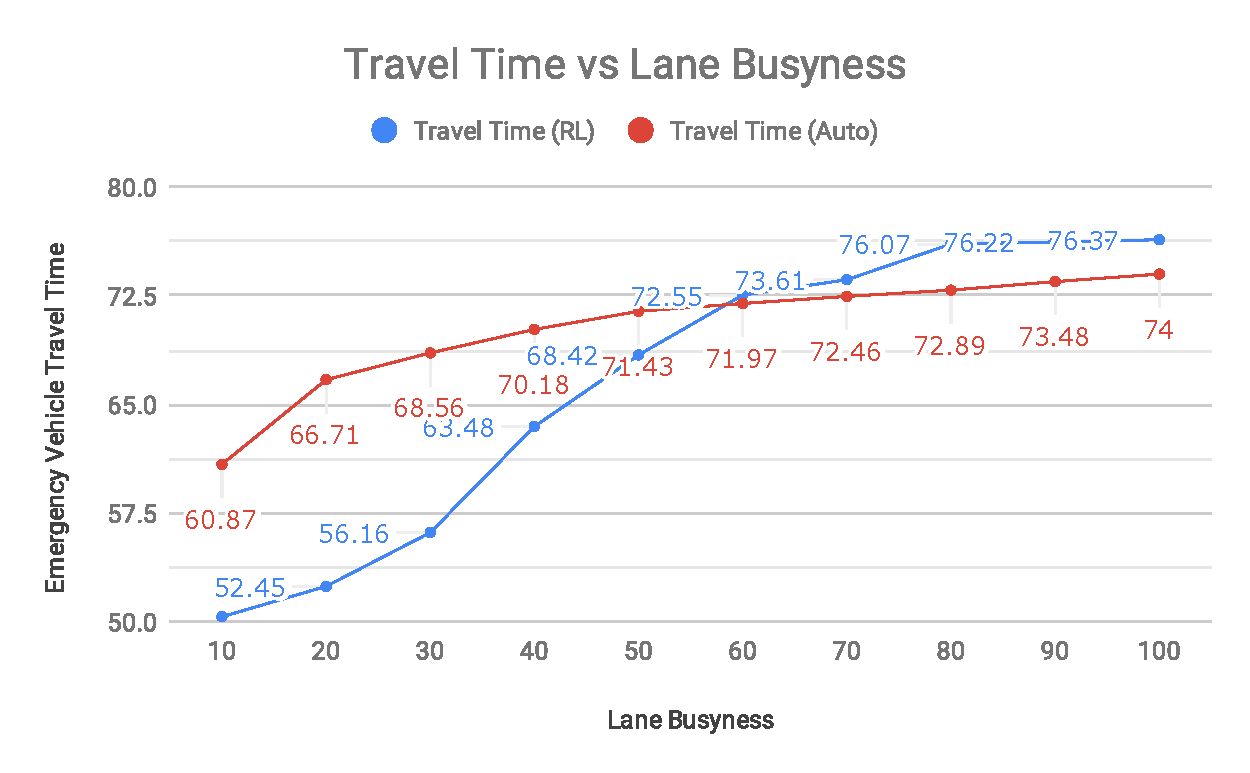
\includegraphics[width=\textwidth]{images/Travel Time vs Lane Busyness.pdf}
    \caption{Travel Time vs Lane Busyness, comparing between two cases: RL (all vehicles on field have the model Q\_LEARNING\_SINGLE\_AGENT) deployed, and Auto(all vehicles on field have the model SUMO\_KRAUSS deployed). Both models described in \ref{sumo_agent_model}.}
    \label{fig:travel_time_vs_lane_busyness_rl_vs_auto}
\end{figure}
\begin{enumerate}
    \item We see clear improvements upon using our model in the EV travel time at low lane busyness's, meeting the SUMO\_KRAUSS model at around 60\% busyness. After which the model almost does not improve the results, and actually results in minimal extra delay.
    \item Abstractly, this is because our approximation of the agent being the only entity responsible for the EV delay\footnote{This approximation is implied by penalizing the agent (check problem formulation) whenever the EV does not used maximum acceleration.} works fine at low busyness's. At higher busyness's, however, the model is unable to change lane because of the absence of lateral free space, nor perform any action  to help the EV accelerate because almost all actions it learned to choose are infeasible (mostly lane changing actions).
    \item Taking further looks at the experiment at higher busyness's, it is evident that the our model vehicle gets trapped trying to perform what it was trained to do: change lane to evacuate the EV's lane. However, because that is not possible and (other times) that is not the solution, it can not do this. 
    \item Furthermore, what makes the performance even worse later is that it has entered unexplored territory: cases that it never sampled during the learning process\footnote{An example case is: the agent being far in front of the EV, but the EV still not having maximum velocity. This is a case that has not been sampled earlier during the learning. Another example is when the agent is just in front of the EV, on its lane, but another vehicle is blocking the lane change so it is infeasible. In the later case, the agent was seen to select random actions, of which one is slowing down.}. In such cases, the agent performs random actions (one of which is slowing down), resulting in the extra delay of the EV.
    \item A key insight due to improvement in lane busyness's: the problem of the lane evacuation is a big problem that communication along with even a simple solutions like this one can result in great improvements at. At 30\% lane busyness for example, only 6.16 time steps (12.3\% of the ideal 50 steps) delay were incurred by the EV when using the RL model, compared to 18.56 steps (37.1\% of the ideal 50 steps) delay incurred by the EV when using the non-communicating\footnote{i.e. are not aware of the presence of the EV.} autonomous vehicles.
    \item Another key insight is that there is still free space to be utilized at high lane busyness's, with the only problem being other AVs blocking any helpful action a single AV could take. Following up with this idea, we believe an independent learner can learn to improve the performance even more, only if trained in presence of other independent learners/vehicles, as another simple solution that could arise would be for agents not on the EV's lane to slow down, allowing for agent's on other lanes to change lane easily.
\end{enumerate}




\item \textbf{Model Performance for Different Lane Busyness's, as RL Percentage Increases}\\
In the last experiment, either all the vehicles used SUMO\_KRAUSS model, or all of them used Q\_LEARNING\_SINGLE\_AGENT model. In this experiment, start from the former cases (all SUMO\_KRAUSS), and increase the percentage of vehicles deploying the Q\_LEARNING\_SINGLE\_AGENT from 0 to 1, with a step of 0.1, to demonstrate the effect of having only some AVs implementing our model. Results are shown in Figure \ref{fig:travel_time_vs_rl_percentages}.\\

\begin{figure}[hbtp]
    \centering
    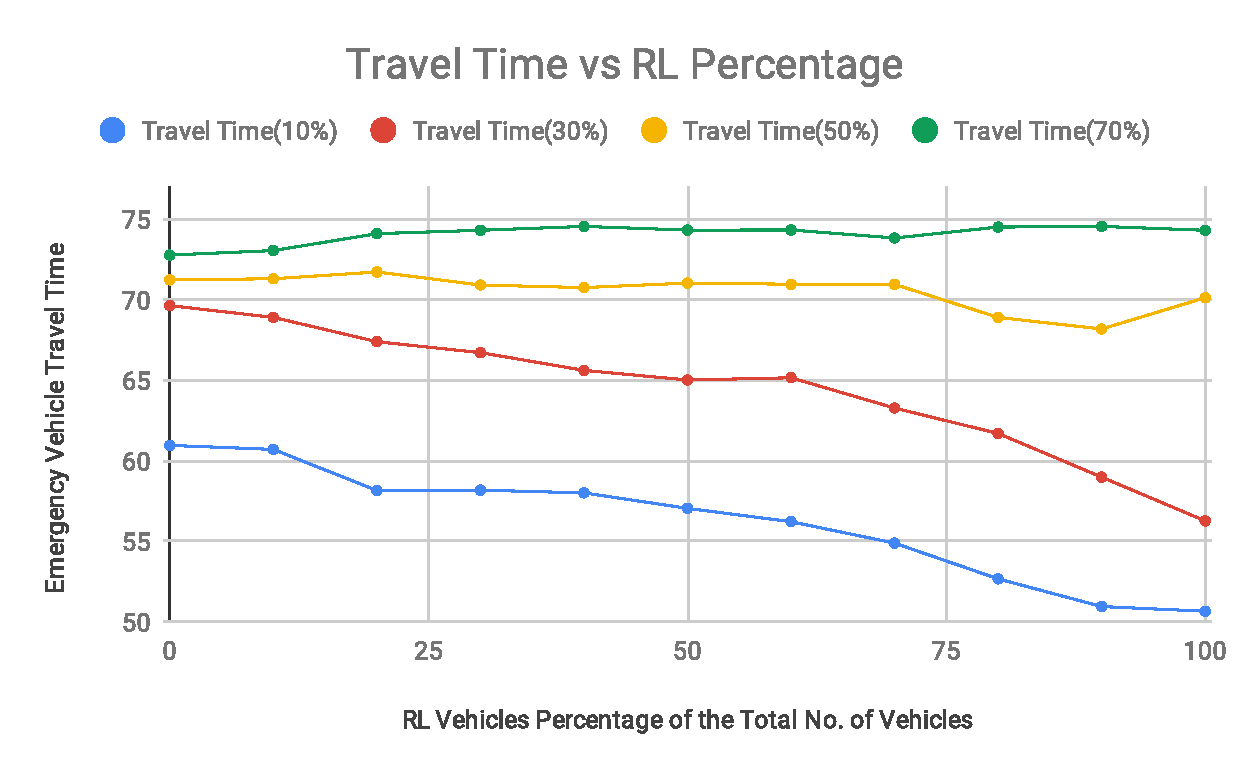
\includegraphics[width=\textwidth]{images/Travel Time vs RL Percentage.pdf}
    \caption{Travel Time vs RL Percentage for different Lane Busyness's.}
    \label{fig:travel_time_vs_rl_percentages}
\end{figure}

Inspecting Figure \ref{fig:travel_time_vs_rl_percentages}, we notice that increasing the percentage of AVs using our model typically monotonically decreases the vehicle travel time. This means that not all vehicles need to be RL vehicles for the system to produce beneficial results, but also that the true benefit of the model appears when more AVs deploy it.





\end{enumerate}


\section{System Integration}
\label{test_final_int}
In this sub-section, we test that our implementation of the single-agent problem on Gazebo, ROS, based on the architecture discussed in \ref{method_integr} allows for a smooth, accurate training of the RL model on one AV which communicates and cooperates with an EV as appropriate. \\ \\
To properly test our architecture, we need to verify the following:
    \begin{enumerate}
    \item The simulation is started, reset and closed successfully.
    \item In case Gazebo dies, the system simulation does not stop and is able to successfully handle the situation.
    \item The environment is able to get the agent's states accurately.
    \item The environment is able to calculate the agent's reward based on its chosen action's execution time.
    \item The environment is able to detect when an episode should be terminated.
    \item The environment is able to detect when the EV is inside/outside the agent's designed window.
    \item Following the RL model is deactivated when the EV is outside the agent's window, and reactivated when it gets inside it.
    \item The agent is not prompted to execute an infeasible action. In such case, a different action is chosen instead.
    \end{enumerate}
To perform the required verifications, the RL model was allowed to be trained for a few episodes in the Gazebo simulation environment. Some chosen parameters were as follows:
\begin{itemize}
    \item The dimensions of the agent's window were set to [-24, 9] meters relative to the agent's position.
    \item The maximum step reward is 0.
    \item Actions are always taken via exploration; since these are the first couple of episodes.
\end{itemize}
The results associated with the significant actions taken by the AV in each of the first 3 episodes were then found to be:

\begin{enumerate}
    \item \textbf{Episode 1}:
    \begin{itemize}
        \item \textbf{Results:}
    \begin{itemize}
        \item \textbf{Episode Termination Reason:} ambulance reached its goal
        \item \textbf{Number of Executed Actions:} 9
        \item \textbf{Final State:}
        \begin{enumerate}
            \item Agent Velocity: 0.144442
            \item Agent Lane: 1
            \item EV Velocity: 0.998572
            \item EV Lane: 2
            \item Relative Position: 17.038090
        \end{enumerate}
        \item \textbf{Initial State:}
        \begin{enumerate}
            \item Agent Velocity: 0.417382
            \item Agent Lane: 0
            \item EV Velocity: 0.967884
            \item EV Lane: 2
            \item Relative Position: -23.068913
        \end{enumerate}
    \end{itemize}
    
    \begin{table} [H]
        \begin{center}
            \begin{tabularx}{1\textwidth} { 
            | >{\raggedright\arraybackslash}p{2cm}
            | >{\raggedright\arraybackslash}p{4.75cm}
            | >{\raggedright\arraybackslash}p{4.75cm} 
            | >{\raggedright\arraybackslash}p{1.75cm}|}
                \hline 
                Requested Action & State Before & State After & Reward \\
                \hline 
                1- Change left was infeasible, then it chose decelerate & \textbf{Agent Velocity:} 0.417382, 
                \newline \textbf{Agent Lane:} 0, 
                \newline \textbf{EV Velocity:} 0.967884, 
                \newline \textbf{EV Lane:} 2, 
                \newline \textbf{Relative Position:} -23.068913 & 
                \textbf{Agent Velocity:} 0.33806, 
                \newline \textbf{Agent Lane:} 0, 
                \newline \textbf{EV Velocity:} 0.999919, 
                \newline \textbf{EV Lane:} 2, 
                \newline \textbf{Relative Position:} -19.848728 & -0.004744 in 5 sec\\
                \hline
                2- No acceleration & \textbf{Agent Velocity:} 0.333763, 
                \newline \textbf{Agent Lane:} 0, 
                \newline \textbf{EV Velocity:} 0.999919, 
                \newline \textbf{EV Lane:} 2, 
                \newline \textbf{Relative Position:} -19.864744 & 
                \textbf{Agent Velocity:} 0.336215, 
                \newline \textbf{Agent Lane:} 0, 
                \newline \textbf{EV Velocity:} 0.999720, 
                \newline \textbf{EV Lane:} 2, 
                \newline \textbf{Relative Position:} -16.504776 & 0 in 5 sec\\
                \hline 
                3- Change left was infeasible, then it chose no acceleration & \textbf{Agent Velocity:} 0.336215, 
                \newline \textbf{Agent Lane:} 0, 
                \newline \textbf{EV Velocity:} 0.999736, 
                \newline \textbf{EV Lane:} 2, 
                \newline \textbf{Relative Position:} -16.485779 & 
                \textbf{Agent Velocity:} 0.336477, 
                \newline \textbf{Agent Lane:} 0, 
                \newline \textbf{EV Velocity:} 0.999372, 
                \newline \textbf{EV Lane:} 2, 
                \newline \textbf{Relative Position:} -13.077777 & 0 in 5 sec\\
                \hline 
                4- Change left was infeasible, then it chose change right & \textbf{Agent Velocity:} 0.336477, 
                \newline \textbf{Agent Lane:} 0, 
                \newline \textbf{EV Velocity:} 0.999372, 
                \newline \textbf{EV Lane:} 2, 
                \newline \textbf{Relative Position:} -13.077777 & 
                \textbf{Agent Velocity:} 0.334250, 
                \newline \textbf{Agent Lane:} 1, 
                \newline \textbf{EV Velocity:} 0.999839, 
                \newline \textbf{EV Lane:} 2, 
                \newline \textbf{Relative Position:} -9.206767 &  0 in 5.7 sec\\
                \hline
            \end{tabularx}
        \caption{#TITLE#: Episode 1 - Results}
        \label{table:episode1}
    \end{center}
    \end{table} 

    %%%%%%%%%%%%%%%%%put here images%%%%%%%%%%%%%%%%
    \begin{figure}[htbp]
    \centering
    \begin{subfigure}[t]{0.3\textwidth}
        \centering
        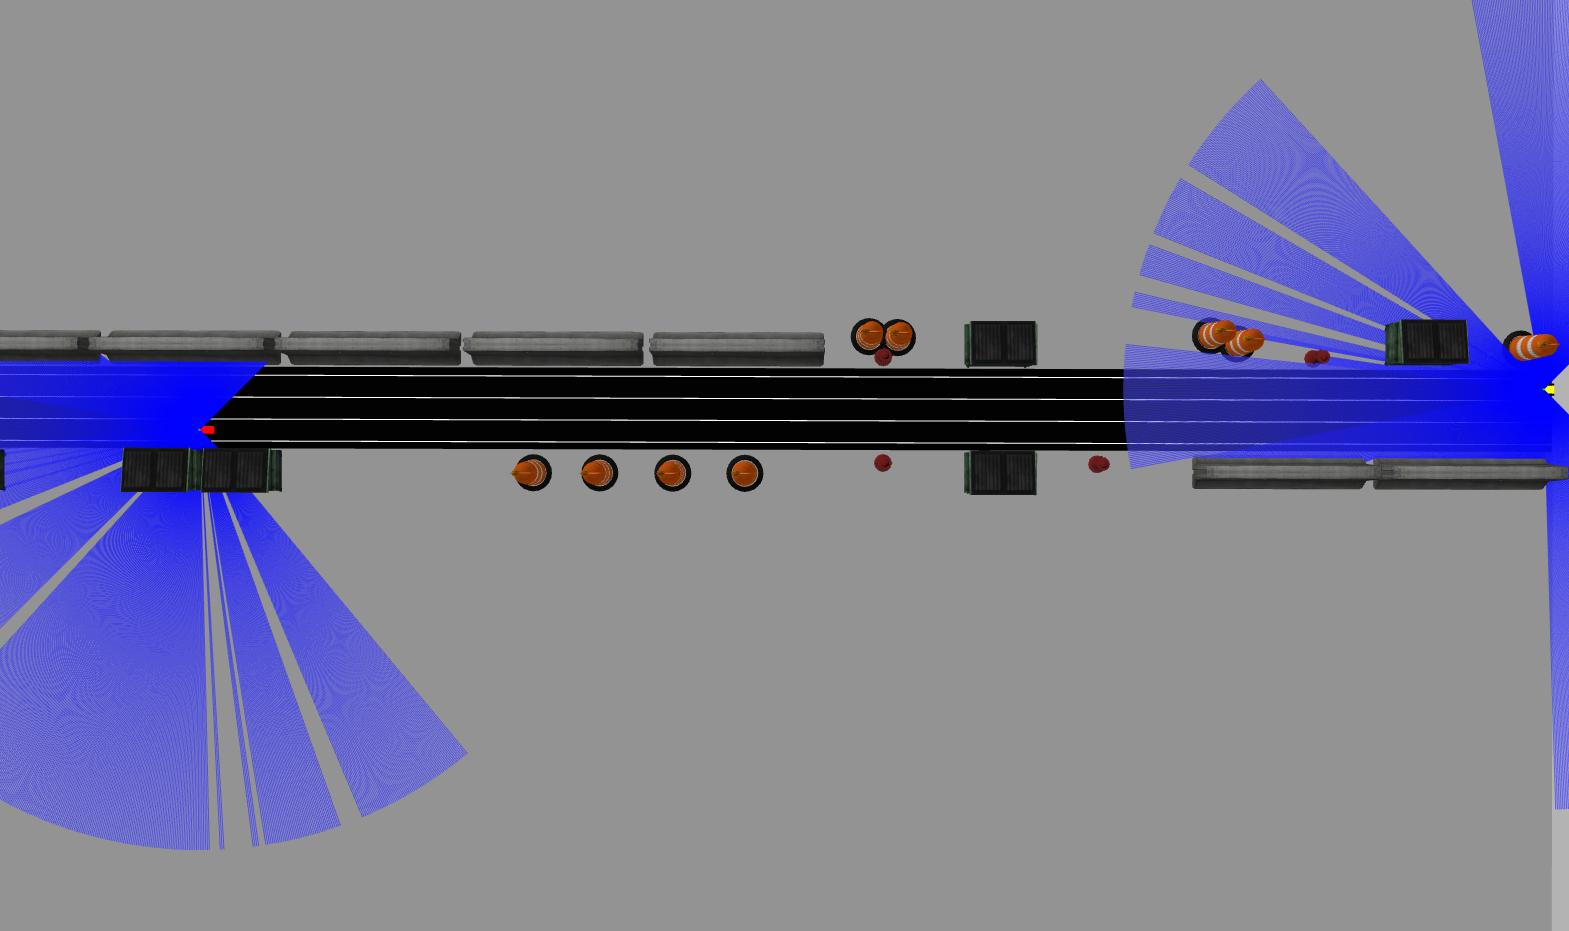
\includegraphics[width=1\linewidth]{images/RLonROS_Test/Episode 1/0start.jpg}
        \caption{Time-step: 0 - Action: Start.}
        \label{fig:RLonROS_Epis1_TS0_start}
    \end{subfigure}\hfil
    \begin{subfigure}[t]{0.3\textwidth}
        \centering
        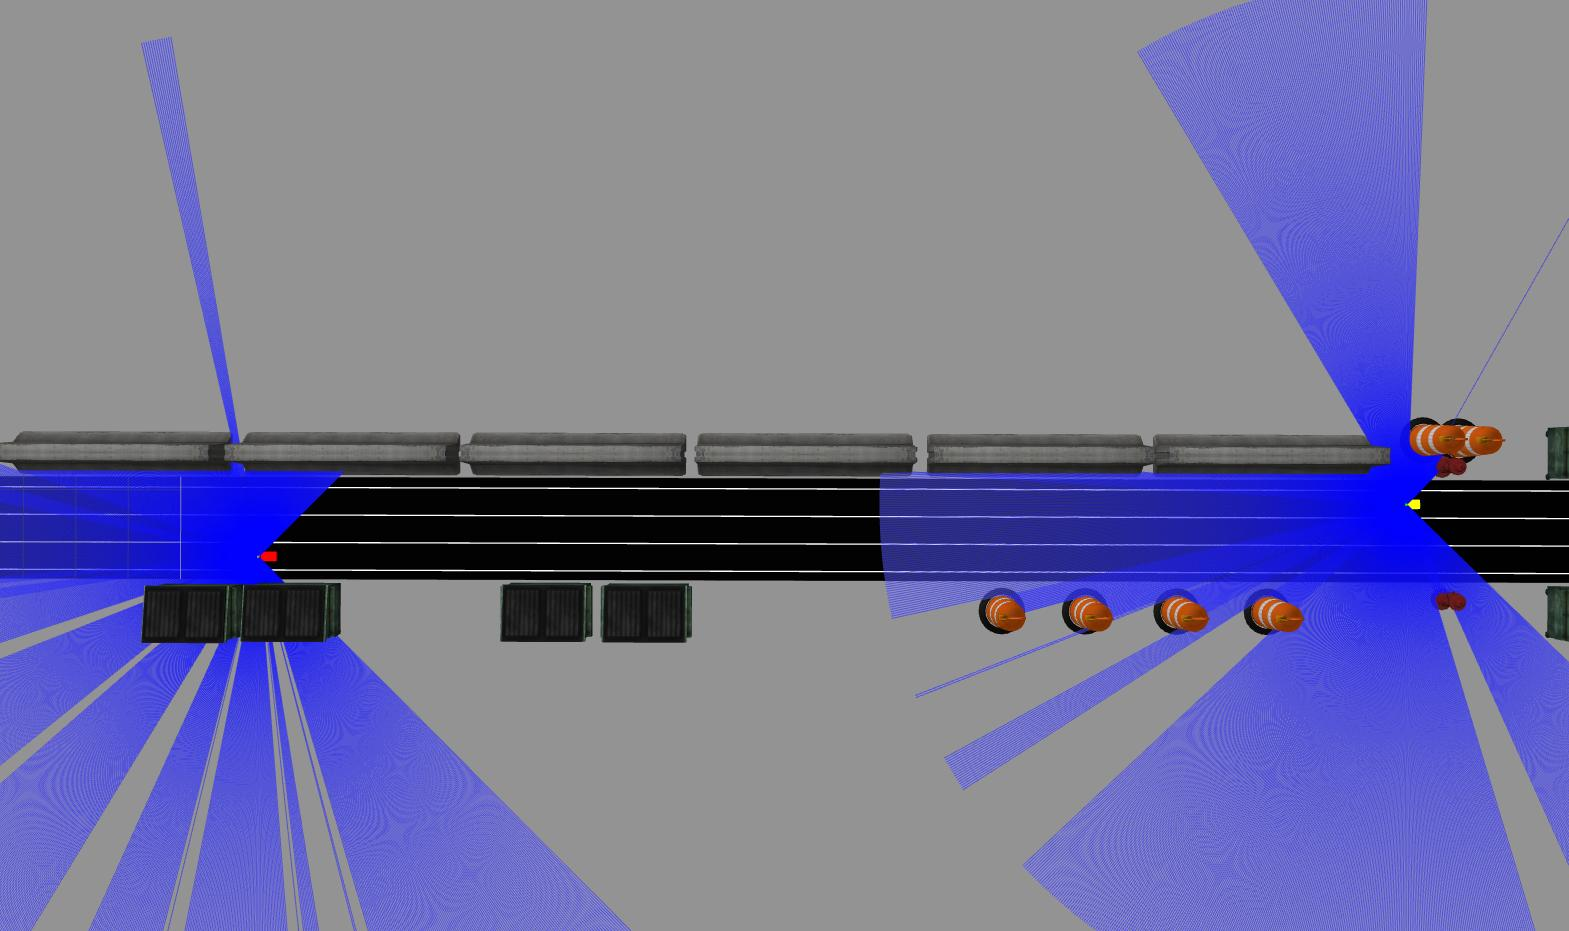
\includegraphics[width=1\linewidth]{images/RLonROS_Test/Episode 1/1Dec.jpg}
        \caption{Time-step: 1 - Action: Deceleration.}
        \label{fig:RLonROS_Epis1_TS1_DEC}
    \end{subfigure}\hfil
    \begin{subfigure}[t]{0.3\textwidth}
        \centering
        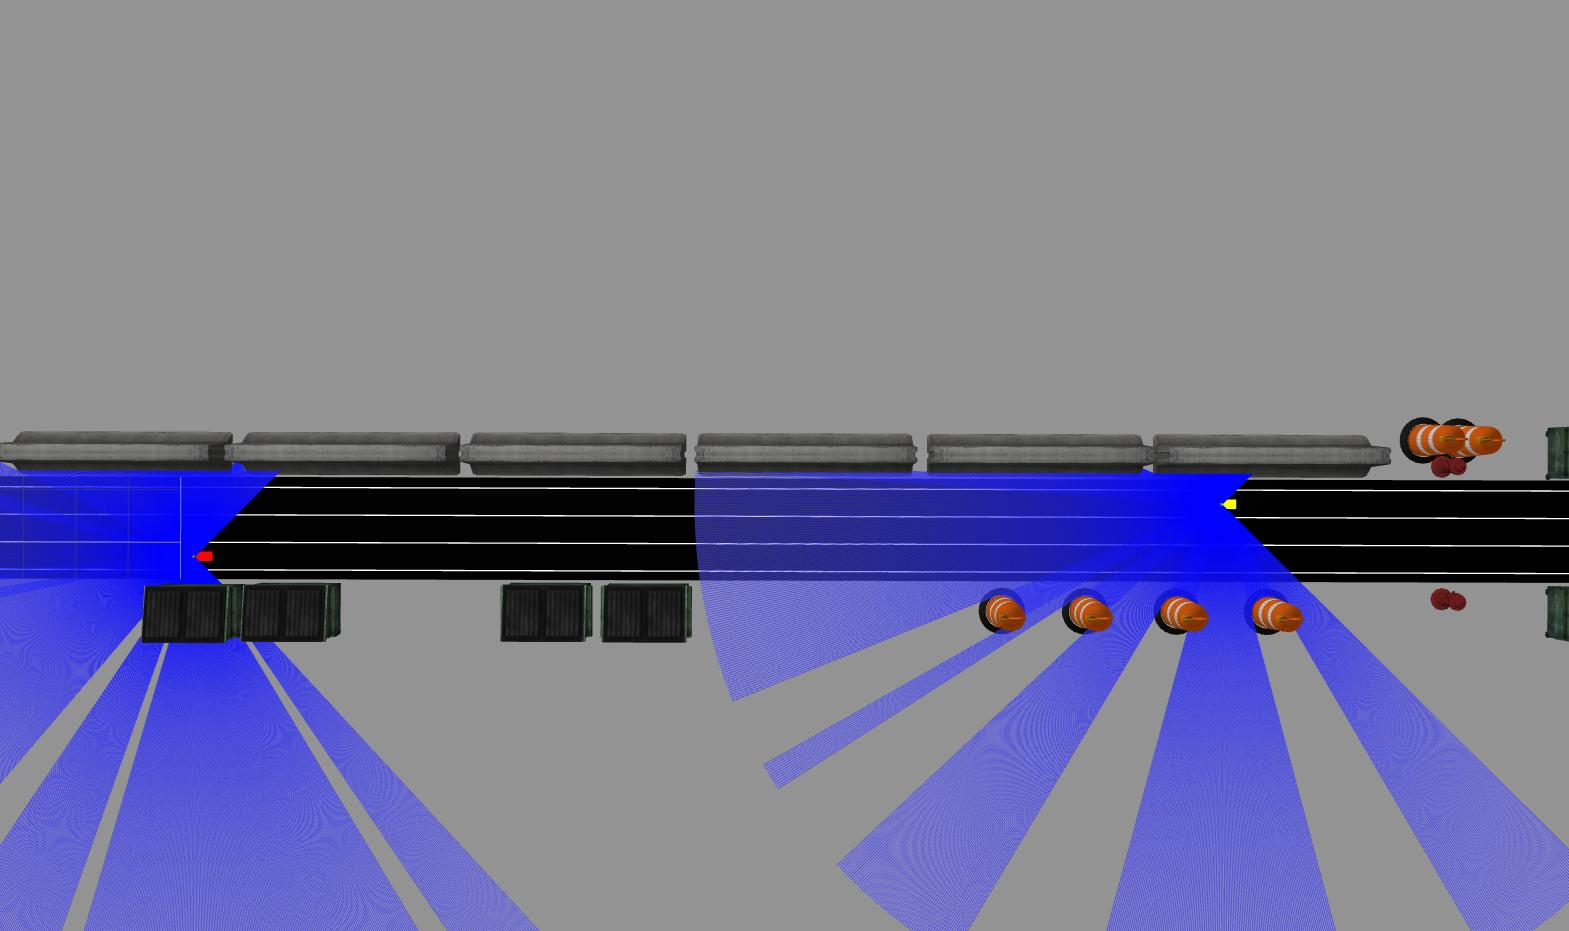
\includegraphics[width=1\linewidth]{images/RLonROS_Test/Episode 1/2NoAcc.jpg}
        \caption{Time-step: 2 - Action: No Action.}
        \label{fig:RLonROS_Epis1_TS2_NOAcc}
    \end{subfigure}\hfil
    %\vspace{1cm} % don't recommend to use it
    \begin{subfigure}[t]{0.3\textwidth}
        \centering
        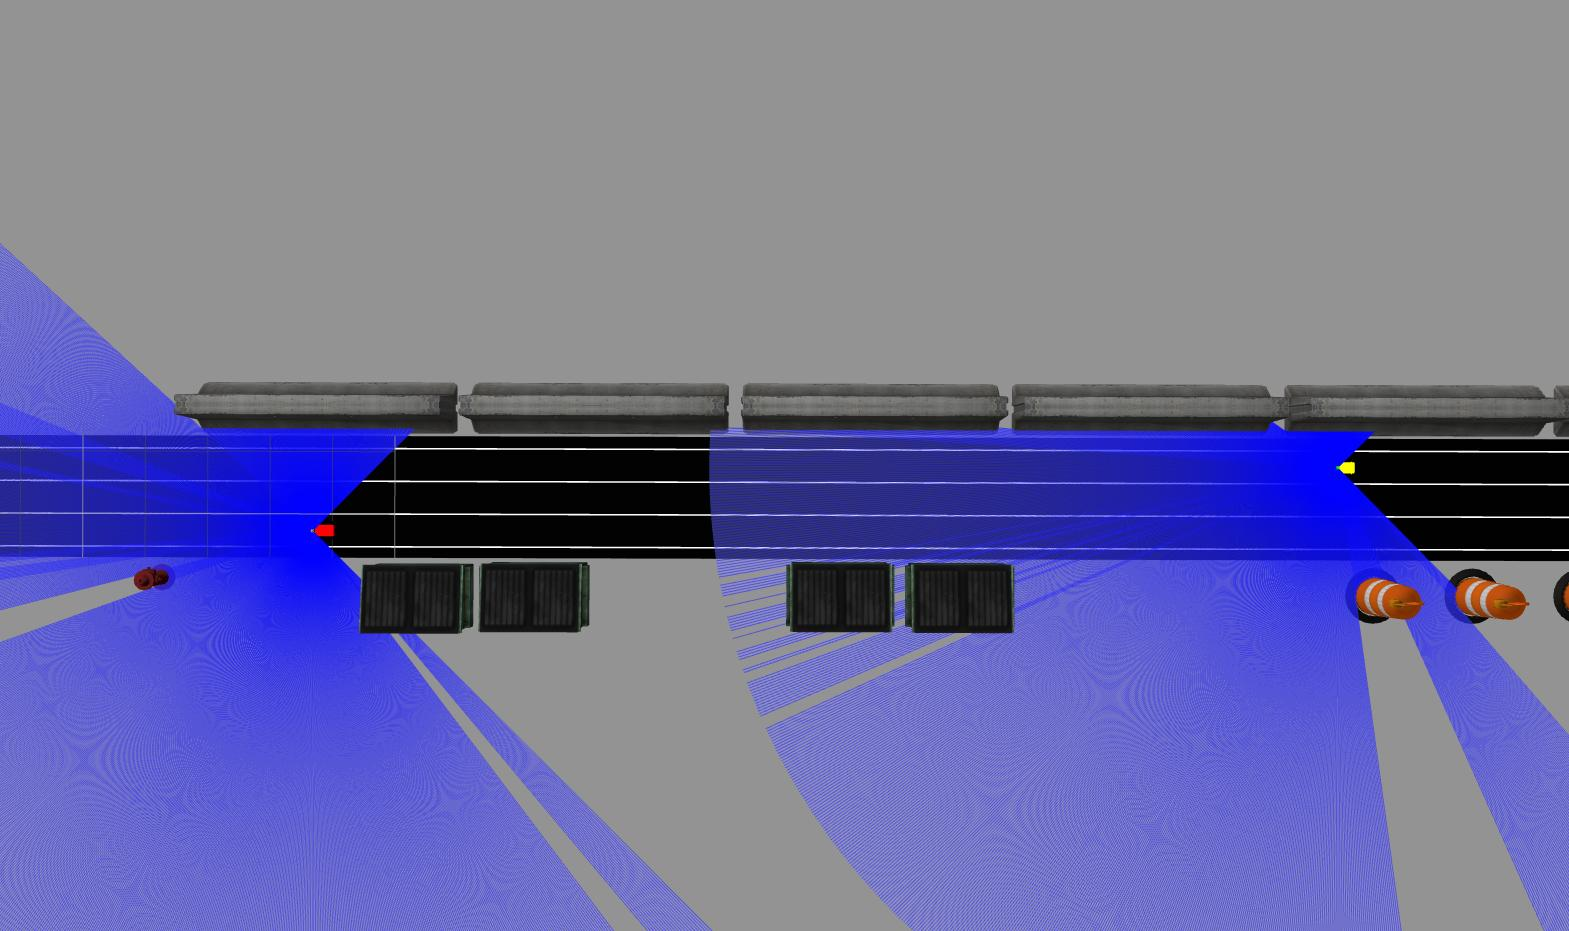
\includegraphics[width=1\linewidth]{images/RLonROS_Test/Episode 1/3NoAcc.jpg}
        \caption{Time-step: 3 - Action: No Action.}
        \label{fig:RLonROS_Epis1_TS3_NOAcc}
    \end{subfigure}\hfil
    \begin{subfigure}[t]{0.3\textwidth}
        \centering
        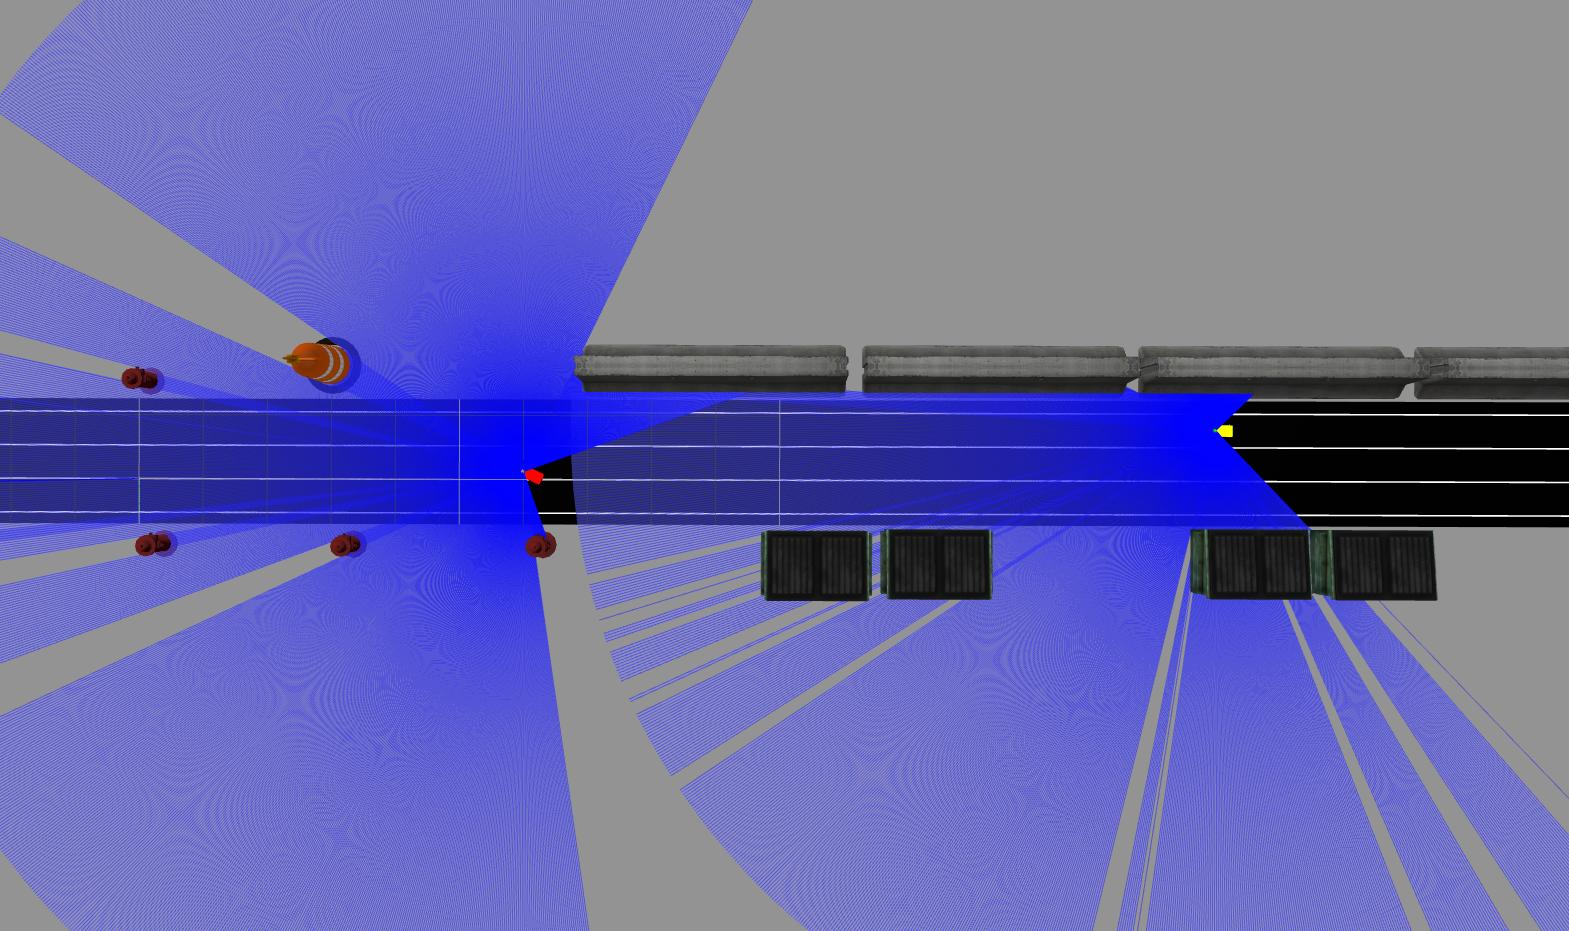
\includegraphics[width=1\linewidth]{images/RLonROS_Test/Episode 1/4changeRight.jpg}
        \caption{Time-step: 4 - Action: Change Right.}
      
        \label{fig:RLonROS_Epis1_TS4_chRight}
    \end{subfigure}\hfil
    \caption{First four time-steps in episode 1.}
    \label{fig:RLonROS_Epis1}
    \end{figure}
    %%%%%%%%%%%%%%%%%DISCUSS HERE%%%%%%%%%%%%%%%%
    \item \textbf{Discussion:}
    \begin{itemize}
        \item It can be noticed in Table \ref{table:episode1} that all actions took place while the relative position between the EV and the agent is greater that -23 and less than -9.3; this validates that the RL model was followed only when the EV is inside the agent's window.
        \item In actions 1, 3 and 4, the first chosen action was lane changing to the left. It was then found to be infeasible (which is true since the agent is already in the left-most lane of the track) and another feasible action was chosen and executed.
        \item The transition between the values of the states is reasonable relative to the taken action.
        \item The state after taking an action in one time step is close to the state before taking an action in the following time step; which means that the designed integrated system architecture takes care of synchronization.
        \item The rewards of actions 2, 3 and 4 are equivalent to the maximum step reward; which is as expected since the velocity of the EV before taking the actions was already maximum and remained so after the actions execution. The reward of action 1 is very close to that of maximum step reward; which is reasonable since the EV performed maximum acceleration.
    \end{itemize}
    \label{rl_on_ros_e1_disc}
    \end{itemize}
    
    \item \textbf{Episode 2}:
    \begin{itemize}
        \item \textbf{Results:}
        \textbf{Episode Termination Reason:} simulation died
        
        \item \textbf{Discussion:}
        Although the Gazebo simulator crashed, the system did not freeze. Instead, the episode was forced to terminate and the simulation was prompted to restart.
    \end{itemize}

    \item \textbf{Episode 3}:
    \begin{itemize}
    \item \textbf{Results:}
    \begin{itemize}
        \item \textbf{Episode Termination Reason:} agent reached its goal
        \item \textbf{Number of Executed Actions:} 9
        \item \textbf{Final State:}
        \begin{enumerate}
            \item Agent Velocity: 0.015078
            \item Agent Lane: 1
            \item EV Velocity: 0.102960
            \item EV Lane: 1
            \item Relative Position: -0.795270
        \end{enumerate}
        \item \textbf{Initial State:}
        \begin{enumerate}
            \item Agent Velocity: 0.416254
            \item Agent Lane: 1
            \item EV Velocity: 0.996863
            \item EV Lane: 1
            \item Relative Position: -22.961435
        \end{enumerate}
    \end{itemize}
 
 \begin{table} [H]
        \begin{center}
            \begin{tabularx}{1\textwidth} { 
            | >{\raggedright\arraybackslash}p{2cm}
            | >{\raggedright\arraybackslash}p{4.75cm}
            | >{\raggedright\arraybackslash}p{4.75cm} 
            | >{\raggedright\arraybackslash}p{1.75cm}|}
                \hline 
                Requested Action & State Before & States After & Reward \\
                \hline 
                1- Decelerate & \textbf{Agent Velocity:} 0.249905, 
                \newline \textbf{Agent Lane:} 1, 
                \newline \textbf{EV Velocity:} 1.000747, 
                \newline \textbf{EV Lane:} 1, 
                \newline \textbf{Relative Position:} -16.362143 & 
                \textbf{Agent Velocity:} 0.149595, 
                \newline \textbf{Agent Lane:} 1, 
                \newline \textbf{EV Velocity:} 0.919836, 
                \newline \textbf{EV Lane:} 1, 
                \newline \textbf{Relative Position:} -12.401335 & -0.584236 in 5 sec\\
                \hline
                2- No acceleration & \textbf{Agent Velocity:} 0.149595, 
                \newline \textbf{Agent Lane:} 1, 
                \newline \textbf{EV Velocity:} 0.919836, 
                \newline \textbf{EV Lane:} 1, 
                \newline \textbf{Relative Position:} -12.4013354 & 
                \textbf{Agent Velocity:} 0.149030, 
                \newline \textbf{Agent Lane:} 1, 
                \newline \textbf{EV Velocity:} 0.778528, 
                \newline \textbf{EV Lane:} 1, 
                \newline \textbf{Relative Position:} -8.794250 & -0.655530 in 5 sec\\
                \hline 
                3- Decelerate & \textbf{Agent Velocity:} 0.149030, 
                \newline \textbf{Agent Lane:} 1, 
                \newline \textbf{EV Velocity:} 0.778528, 
                \newline \textbf{EV Lane:} 1, 
                \newline \textbf{Relative Position:} -8.794250 & 
                \textbf{Agent Velocity:} 0.048788, 
                \newline \textbf{Agent Lane:} 1, 
                \newline \textbf{EV Velocity:} 0.600992, 
                \newline \textbf{EV Lane:} 1, 
                \newline \textbf{Relative Position:} -5.818396 & -0.790863 in 5 sec\\
                \hline 
                4- Decelerate & \textbf{Agent Velocity:} 0.048788, 
                \newline \textbf{Agent Lane:} 1, 
                \newline \textbf{EV Velocity:} 0.601142, 
                \newline \textbf{EV Lane:} 1, 
                \newline \textbf{Relative Position:} -5.788945 & 
                \textbf{Agent Velocity:} 0.015384, 
                \newline \textbf{Agent Lane:} 1, 
                \newline \textbf{EV Velocity:} 0.563688, 
                \newline \textbf{EV Lane:} 1, 
                \newline \textbf{Relative Position:} -4.905980 &  -0.861758 in 5 sec\\
                \hline
            \end{tabularx}
        \caption{Episode 3 results}
        \label{table:episode3}
    \end{center}
    \end{table} 
    
    %%%%%%%%%%%%%%%%%put here images%%%%%%%%%%%%%%%%
    \begin{figure}[htbp]
    \centering
    \begin{subfigure}[t]{0.3\textwidth}
        \centering
        
\includegraphics[width=1\linewidth]{images/RLonROS_Test/Episode 3/0start.jpg}
        \caption{Time-step: 0 - Start.}
        \label{fig:RLonROS_Epis3_TS0_start}
    \end{subfigure}\hfil
    \begin{subfigure}[t]{0.3\textwidth}
        \centering
        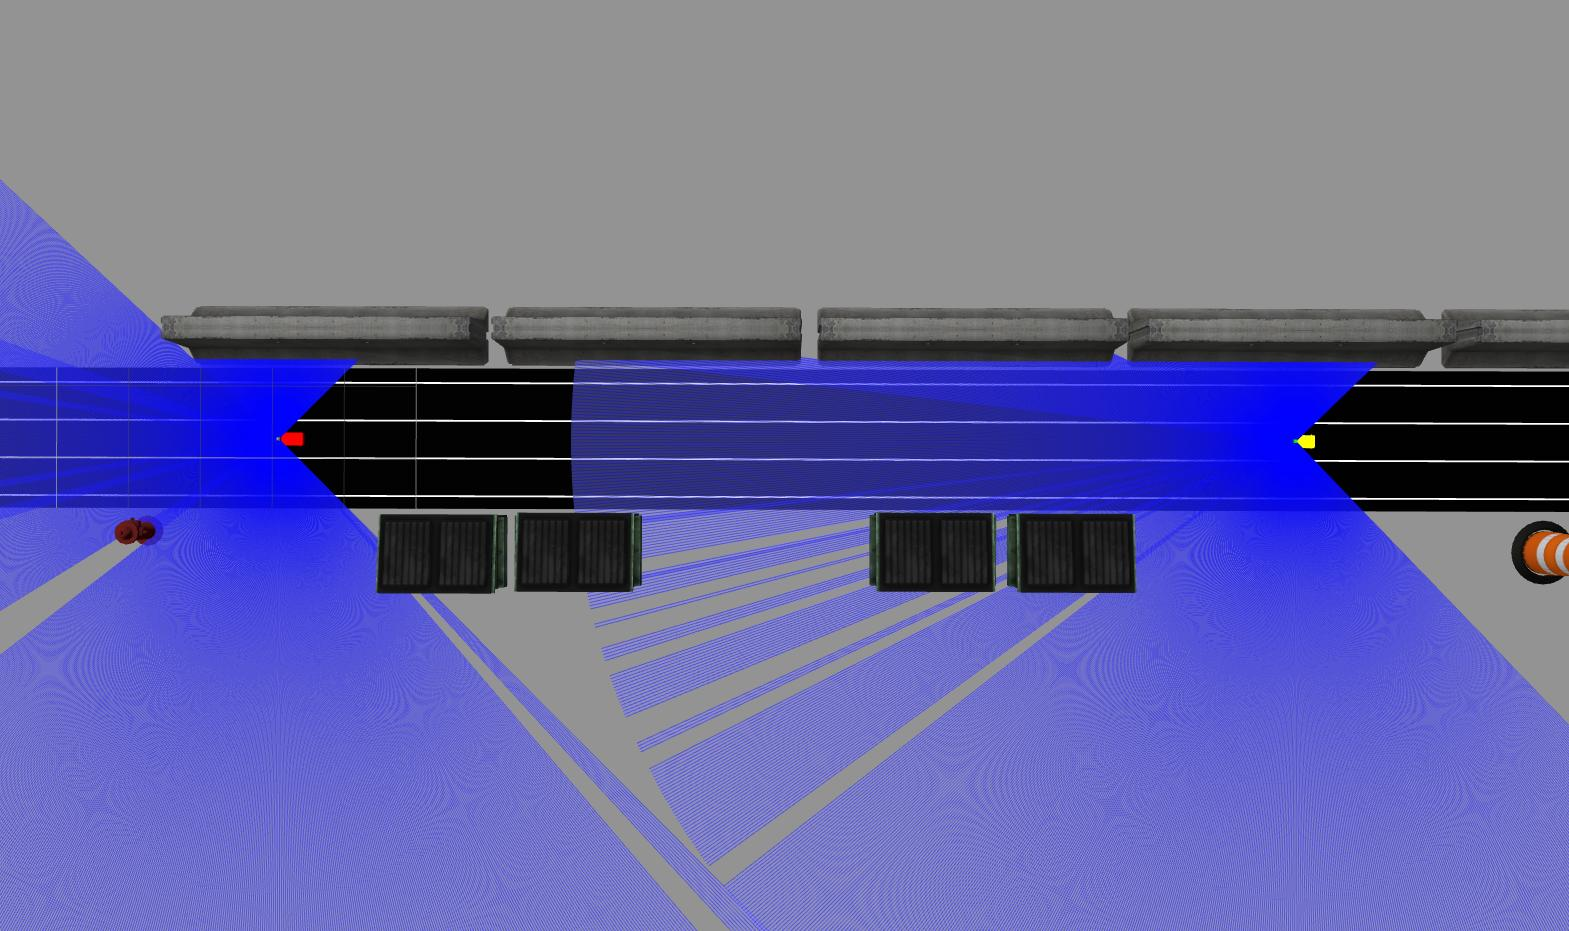
\includegraphics[width=1\linewidth]{images/RLonROS_Test/Episode 3/1dec.jpg}
        \caption{Time-step: 1 - Action: Deceleration.}
        \label{fig:RLonROS_Epis3_TS1_DEC}
    \end{subfigure}\hfil
    \begin{subfigure}[t]{0.3\textwidth}
        \centering
        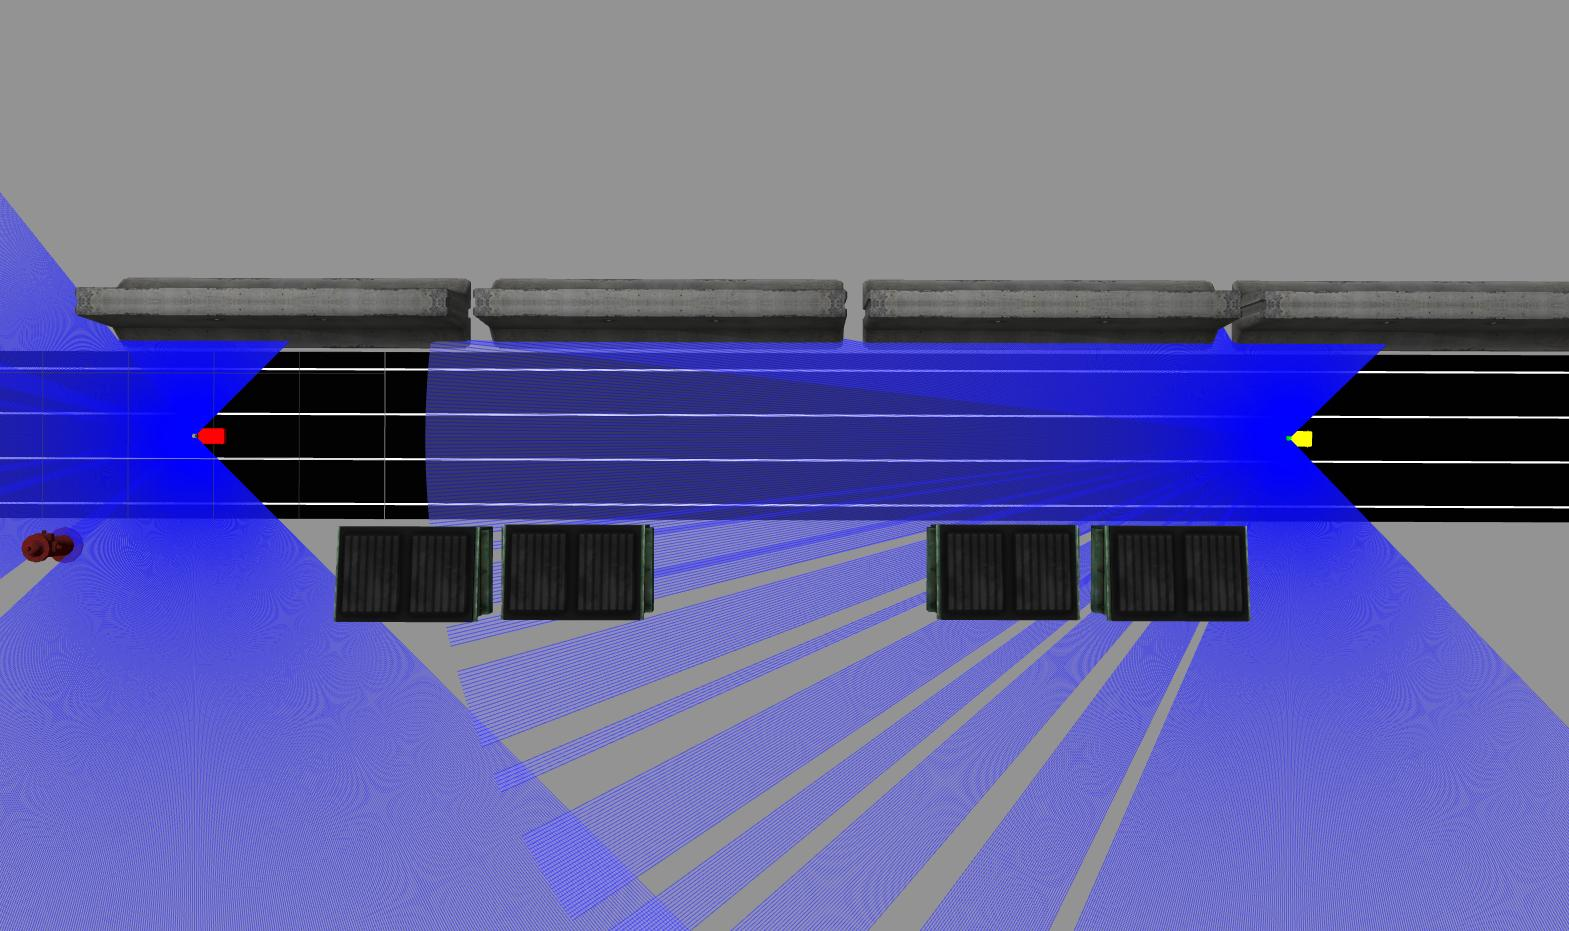
\includegraphics[width=1\linewidth]{images/RLonROS_Test/Episode 3/2noacc.jpg}
        \caption{Time-step: 2 - Action: No Action.}
        \label{fig:RLonROS_Epis3_TS2_NOAcc}
    \end{subfigure}\hfil
    \begin{subfigure}[t]{0.3\textwidth}
        \centering
        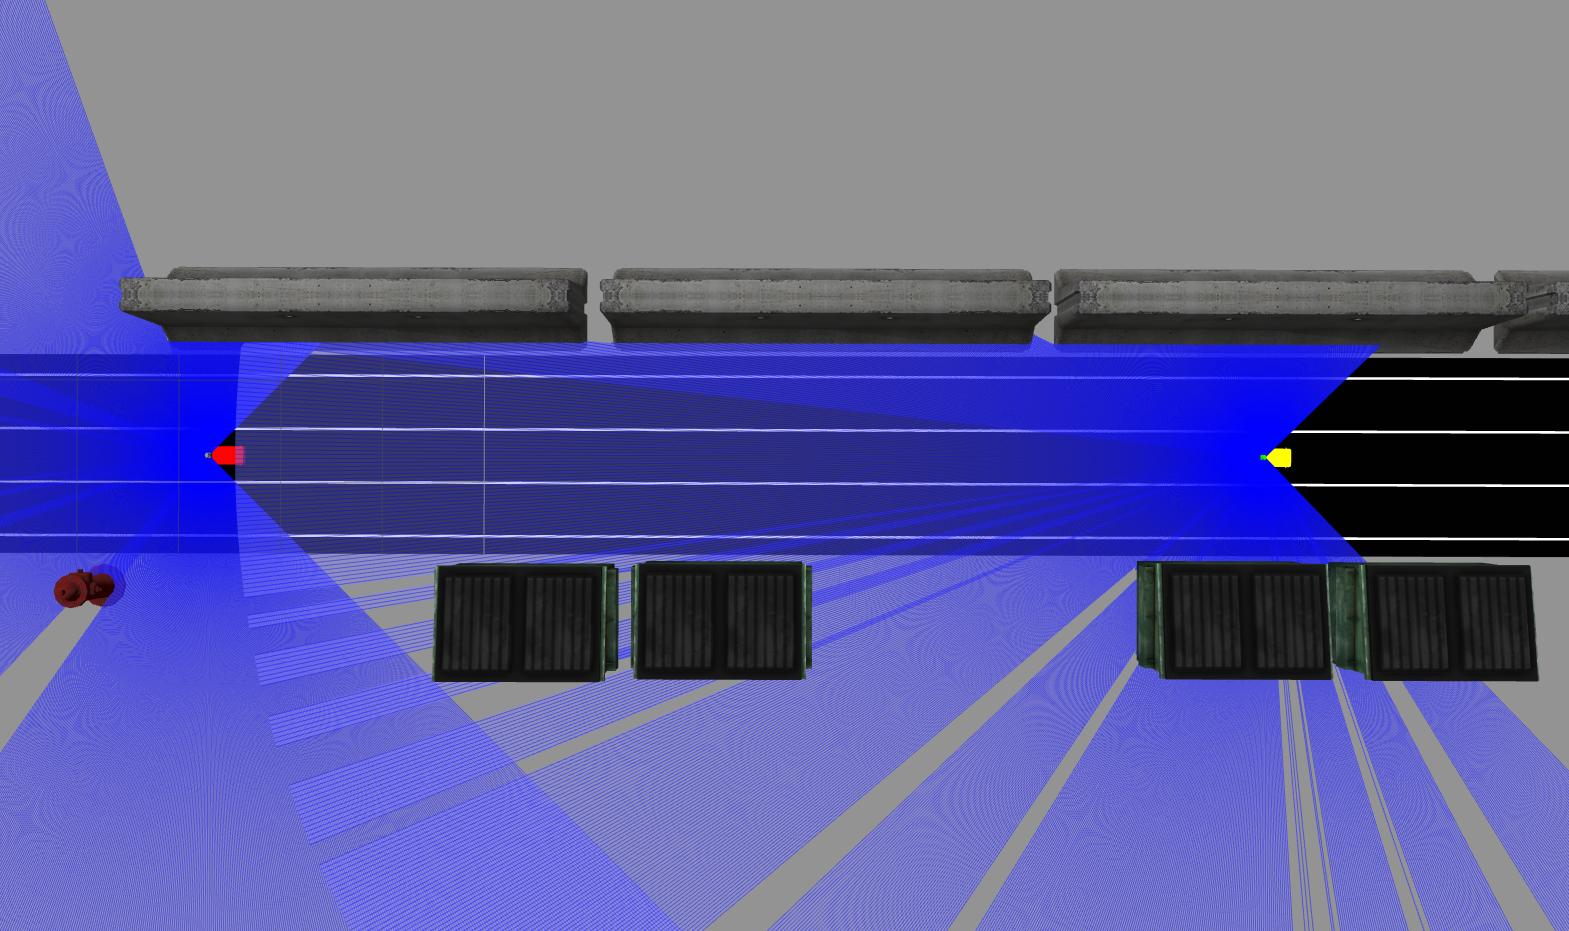
\includegraphics[width=1\linewidth]{images/RLonROS_Test/Episode 3/3dec.jpg}
        \caption{Time-step: 3 - Action: Deceleration.}
        \label{fig:RLonROS_Epis3_TS3_DEC}
    \end{subfigure}\hfil
    \begin{subfigure}[t]{0.3\textwidth}
        \centering
        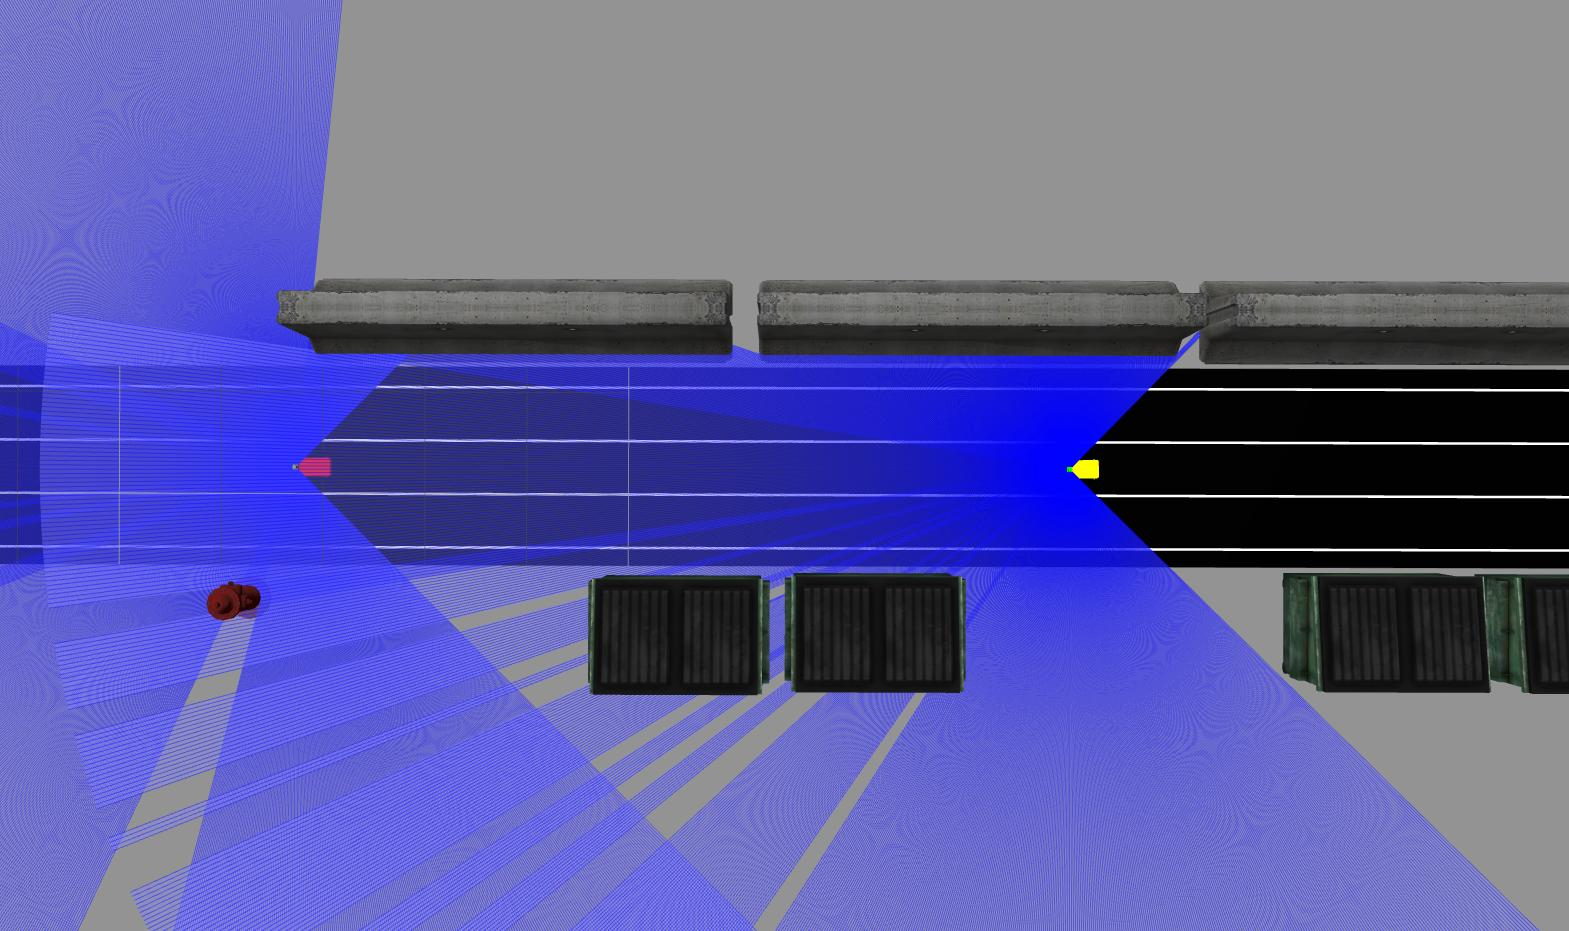
\includegraphics[width=1\linewidth]{images/RLonROS_Test/Episode 3/4dec.jpg}
        \caption{Time-step: 4 - Action: Deceleration.}
        \label{fig:RLonROS_Epis3_TS4_DEC}
    \end{subfigure}\hfil
    \caption{First four time-steps in episode 3.}
    \label{fig:RLonROS_Epis3}
    \end{figure}
    \item \textbf{Discussion:}
        \begin{itemize}
        \item Apart from comments similar to those in \ref{rl_on_ros_e1_disc}, it is clear in Table \ref{table:episode3} that when the agent was preceding the EV in the same lane, the EV has to reduce its velocity in order to keep a safe distance between the agent and itself. As a result of such a decrease in EV velocity, the agent was given negative reward.
        \end{itemize}
    \end{itemize}
    \item \textbf{General Discussion:}
    \begin{itemize}
        \item Between episodes, the simulation was smoothly restarted and the vehicles' initial positions and final goals were reset correctly.
        \item Although the different system components were tested and found to be working, one important aspect to further test before fully training the RL model is the effect of the reward normalization based on action execution times. Thorough testing is needed in order to make sure that no undesirable behaviors accordingly arise. 
    \end{itemize}
\end{enumerate}